% ============================================================
% BRITISH ENGLISH PROFICIENCY PROGRAMME
% 12-Month Intensive Programme — 2 Hours Daily
% Preamble
% ============================================================
\ifdefined\VowelsStandalonefalse\else
\documentclass[
    12pt,
    a4paper,
    oneside,
    openany
]{book}
\usepackage{fontspec}
\setmainfont{DejaVu Serif}
\setmonofont{DejaVu Sans Mono}
\usepackage[british]{babel}

\usepackage{geometry}
\geometry{margin=27mm}
\usepackage{longtable,booktabs,array,tabularx,multicol,enumitem}
\usepackage{xcolor,graphicx,hyperref,fancyhdr,tcolorbox}
\tcbuselibrary{breakable,skins}
\hypersetup{colorlinks=true,linkcolor=blue!45!black,urlcolor=blue!50!black}
\newcommand{\ipa}[1]{{\fontspec{DejaVu Sans}/#1/}}
\newcommand{\res}[3]{\begin{tcolorbox}[breakable,colback=gray!5,colframe=gray!55,title={Resource placeholder: #1}]\textbf{Deliverable:} #2\par\textbf{Specification:} #3\end{tcolorbox}}
\newcommand{\task}[2]{\begin{tcolorbox}[breakable,colback=blue!2,colframe=blue!45!black,title={Practice: #1}]#2\end{tcolorbox}}
\newcommand{\checkline}{\par\noindent\rule{\linewidth}{0.35pt}\par}
\setcounter{tocdepth}{2}



% ============================================================
% ENCODING AND LANGUAGE
% ============================================================

\usepackage[T1]{fontenc}
\usepackage[utf8]{inputenc}

\usepackage[
    british,
    main=british
]{babel}

\usepackage{lmodern}
\usepackage{microtype}

% ============================================================
% PAGE GEOMETRY
% ============================================================

\usepackage[
    top=2.5cm,
    bottom=2.5cm,
    inner=3cm,
    outer=2.5cm,
    headheight=15pt,
    headsep=0.8cm,
    footskip=1.2cm
]{geometry}

% ============================================================
% TYPOGRAPHY AND PARAGRAPH FORMATTING
% ============================================================

\usepackage{setspace}

\setstretch{1.15}

\setlength{\parindent}{0pt}
\setlength{\parskip}{0.6em}

\usepackage{ragged2e}

% ============================================================
% COLOURS
% ============================================================

\usepackage{xcolor}

\definecolor{BritishNavy}{HTML}{012169}
\definecolor{BritishRed}{HTML}{C8102E}
\definecolor{DarkGrey}{HTML}{333333}
\definecolor{MediumGrey}{HTML}{666666}
\definecolor{LightGrey}{HTML}{F3F4F6}
\definecolor{VeryLightBlue}{HTML}{EEF3FA}
\definecolor{PracticeGreen}{HTML}{2E7D32}
\definecolor{WarningOrange}{HTML}{C65D00}

% ============================================================
% GRAPHICS
% ============================================================

\usepackage{graphicx}
\usepackage{float}
\usepackage{subcaption}

\graphicspath{{images/}{figures/}{assets/}}

% ============================================================
% TABLES
% ============================================================

\usepackage{booktabs}
\usepackage{tabularx}
\usepackage{longtable}
\usepackage{multirow}
\usepackage{array}
\usepackage{colortbl}
\usepackage{makecell}

\renewcommand{\arraystretch}{1.2}

% ============================================================
% LISTS
% ============================================================

\usepackage{enumitem}

\setlist[itemize]{
    leftmargin=1.5em,
    itemsep=0.25em,
    topsep=0.4em
}

\setlist[enumerate]{
    leftmargin=1.8em,
    itemsep=0.25em,
    topsep=0.4em
}

% ============================================================
% MATHEMATICS AND SYMBOLS
% ============================================================

\usepackage{amsmath}
\usepackage{amssymb}
\usepackage{mathtools}

% ============================================================
% PHONETICS / IPA
% ============================================================

\usepackage{tipa}

% Examples:
% \textipa{/I/}
% \textipa{/i:/}
% \textipa{/T/}
% \textipa{/D/}
% \textipa{/S/}
% \textipa{/Z/}

% ============================================================
% HEADINGS
% ============================================================

\usepackage{titlesec}

\titleformat{\chapter}[display]
    {\normalfont\bfseries\color{BritishNavy}}
    {\Large\chaptername\ \thechapter}
    {0.5em}
    {\Huge}

\titleformat{\section}
    {\Large\bfseries\color{BritishNavy}}
    {\thesection}
    {0.75em}
    {}

\titleformat{\subsection}
    {\large\bfseries\color{BritishRed}}
    {\thesubsection}
    {0.75em}
    {}

\titleformat{\subsubsection}
    {\normalsize\bfseries\color{DarkGrey}}
    {\thesubsubsection}
    {0.75em}
    {}

\setcounter{secnumdepth}{3}
\setcounter{tocdepth}{3}

% ============================================================
% HEADER AND FOOTER
% ============================================================

\usepackage{fancyhdr}

\pagestyle{fancy}
\fancyhf{}

\fancyhead[L]{
    \small\textcolor{MediumGrey}{
        British English Proficiency Programme
    }
}

\fancyhead[R]{
    \small\textcolor{MediumGrey}{
        \leftmark
    }
}

\fancyfoot[C]{
    \small\textcolor{MediumGrey}{
        \thepage
    }
}

\renewcommand{\headrulewidth}{0.4pt}
\renewcommand{\footrulewidth}{0pt}

% Chapter-opening pages
\fancypagestyle{plain}{
    \fancyhf{}
    \fancyfoot[C]{\thepage}
    \renewcommand{\headrulewidth}{0pt}
}

% ============================================================
% TABLE OF CONTENTS FORMATTING
% ============================================================

\usepackage{tocloft}

\renewcommand{\cftchapfont}{
    \bfseries\color{BritishNavy}
}

\renewcommand{\cftchappagefont}{
    \bfseries\color{BritishNavy}
}

\renewcommand{\cftsecfont}{
    \color{DarkGrey}
}

\renewcommand{\cftsubsecfont}{
    \color{MediumGrey}
}

\setlength{\cftbeforechapskip}{0.7em}

% ============================================================
% HYPERLINKS AND PDF METADATA
% ============================================================

\usepackage{hyperref}

\hypersetup{
    colorlinks=true,
    linkcolor=BritishNavy,
    citecolor=BritishRed,
    urlcolor=BritishRed,
    pdfauthor={British English Proficiency Programme},
    pdftitle={12-Month Intensive British English Proficiency Programme},
    pdfsubject={
        Received Pronunciation, Speaking, Listening,
        Grammar, Writing and Communication
    },
    pdfkeywords={
        British English,
        Received Pronunciation,
        RP,
        English Learning,
        Speaking,
        Listening,
        Phonetics,
        Grammar,
        Academic Writing
    },
    bookmarksopen=true,
    bookmarksnumbered=true
}

\usepackage{bookmark}

% ============================================================
% BOXES FOR LESSONS, EXERCISES, NOTES, ETC.
% ============================================================

\usepackage[
    most
]{tcolorbox}

% ------------------------------------------------------------
% Learning objectives
% ------------------------------------------------------------

\newtcolorbox{learningobjectives}{
    enhanced,
    breakable,
    colback=VeryLightBlue,
    colframe=BritishNavy,
    title=\textbf{Learning Objectives},
    fonttitle=\bfseries,
    arc=2mm,
    boxrule=0.8pt
}

% ------------------------------------------------------------
% Pronunciation focus
% ------------------------------------------------------------

\newtcolorbox{pronunciation}{
    enhanced,
    breakable,
    colback=LightGrey,
    colframe=BritishRed,
    title=\textbf{Pronunciation Focus},
    fonttitle=\bfseries,
    arc=2mm,
    boxrule=0.8pt
}

% ------------------------------------------------------------
% Speaking practice
% ------------------------------------------------------------

\newtcolorbox{speakingpractice}{
    enhanced,
    breakable,
    colback=VeryLightBlue,
    colframe=PracticeGreen,
    title=\textbf{Speaking Practice},
    fonttitle=\bfseries,
    arc=2mm,
    boxrule=0.8pt
}

% ------------------------------------------------------------
% Listening practice
% ------------------------------------------------------------

\newtcolorbox{listeningpractice}{
    enhanced,
    breakable,
    colback=LightGrey,
    colframe=BritishNavy,
    title=\textbf{Listening Practice},
    fonttitle=\bfseries,
    arc=2mm,
    boxrule=0.8pt
}

% ------------------------------------------------------------
% Grammar focus
% ------------------------------------------------------------

\newtcolorbox{grammarfocus}{
    enhanced,
    breakable,
    colback=VeryLightBlue,
    colframe=DarkGrey,
    title=\textbf{Grammar Focus},
    fonttitle=\bfseries,
    arc=2mm,
    boxrule=0.8pt
}

% ------------------------------------------------------------
% Vocabulary
% ------------------------------------------------------------

\newtcolorbox{vocabularybox}{
    enhanced,
    breakable,
    colback=LightGrey,
    colframe=PracticeGreen,
    title=\textbf{Vocabulary},
    fonttitle=\bfseries,
    arc=2mm,
    boxrule=0.8pt
}

% ------------------------------------------------------------
% Writing practice
% ------------------------------------------------------------

\newtcolorbox{writingpractice}{
    enhanced,
    breakable,
    colback=VeryLightBlue,
    colframe=BritishNavy,
    title=\textbf{Writing Practice},
    fonttitle=\bfseries,
    arc=2mm,
    boxrule=0.8pt
}

% ------------------------------------------------------------
% Assessment
% ------------------------------------------------------------

\newtcolorbox{assessmentbox}{
    enhanced,
    breakable,
    colback=LightGrey,
    colframe=BritishRed,
    title=\textbf{Assessment},
    fonttitle=\bfseries,
    arc=2mm,
    boxrule=0.8pt
}

% ------------------------------------------------------------
% Important note
% ------------------------------------------------------------

\newtcolorbox{importantnote}{
    enhanced,
    breakable,
    colback=LightGrey,
    colframe=WarningOrange,
    title=\textbf{Important},
    fonttitle=\bfseries,
    arc=2mm,
    boxrule=0.8pt
}

% ============================================================
% QUOTES AND DIALOGUES
% ============================================================

\usepackage{csquotes}

% ============================================================
% CUSTOM COMMANDS
% ============================================================

% IPA shortcut
\newcommand{\ipa}[1]{%
    \textipa{/#1/}%
}

% British English term
\newcommand{\british}[1]{%
    \textbf{\textcolor{BritishNavy}{#1}}%
}

% American English comparison
\newcommand{\american}[1]{%
    \textcolor{MediumGrey}{#1}%
}

% Key vocabulary
\newcommand{\keyword}[1]{%
    \textbf{\textcolor{BritishRed}{#1}}%
}

% Pronunciation target
\newcommand{\rptarget}[1]{%
    \textbf{\textcolor{BritishRed}{#1}}%
}

% ============================================================
% DAY / WEEK / MONTH COMMANDS
% ============================================================

\newcommand{\monthheading}[2]{%
    \chapter{Month #1: #2}
}

\newcommand{\weekheading}[2]{%
    \section{Week #1: #2}
}

\newcommand{\dayheading}[2]{%
    \subsection{Day #1: #2}
}

% ============================================================
% DAILY SESSION TEMPLATE
% ============================================================

\newcommand{\dailysession}[1]{%
    \begin{tcolorbox}[
        enhanced,
        breakable,
        colback=white,
        colframe=BritishNavy,
        title=\textbf{Daily Session — #1},
        fonttitle=\bfseries,
        arc=2mm,
        boxrule=1pt
    ]
    \textbf{Recommended duration: 120 minutes}

    \medskip

    \begin{tabularx}{\textwidth}{
        >{\bfseries}p{3.8cm} X
    }
    Pronunciation / Phonetics & 30 minutes \\
    Speaking / Conversation   & 30 minutes \\
    Listening / Comprehension & 25 minutes \\
    Grammar / Vocabulary      & 20 minutes \\
    Writing / Reflection      & 15 minutes \\
    \end{tabularx}
    \end{tcolorbox}
}

% ============================================================
% CEFR LEVEL COMMAND
% ============================================================

\newcommand{\cefr}[1]{%
    \textbf{\textcolor{BritishNavy}{CEFR #1}}%
}

% ============================================================
% CHECKBOXES
% ============================================================

\usepackage{amssymb}

\newcommand{\checkbox}{%
    $\square$
}

\newcommand{\checkedbox}{%
    $\boxtimes$
}

% ============================================================
% DATE / CALENDAR SUPPORT
% ============================================================

\usepackage{datetime2}

% ============================================================
% INDEX
% ============================================================

\usepackage{imakeidx}
\makeindex[
    title=Language and Pronunciation Index,
    columns=2
]

% Usage:
% pronunciation\index{pronunciation}
% schwa\index{schwa}

% ============================================================
% GLOSSARY / ACRONYMS
% ============================================================

\usepackage[
    acronym,
    toc,
    nonumberlist
]{glossaries}

\makeglossaries

\newacronym{rp}{RP}{Received Pronunciation}
\newacronym{ipa}{IPA}{International Phonetic Alphabet}
\newacronym{cefr}{CEFR}{Common European Framework of Reference for Languages}

% ============================================================
% BIBLIOGRAPHY
% ============================================================

\usepackage[
    backend=biber,
    style=apa,
    sorting=nyt
]{biblatex}

% Uncomment when the bibliography file exists:
% \addbibresource{references.bib}

% ============================================================
% TITLE INFORMATION
% ============================================================

\title{
    \Huge
    \textbf{
        British English Proficiency Programme
    }
    \\[0.5cm]
    \Large
    A 12-Month Intensive Programme
    \\[0.2cm]
    \large
    Received Pronunciation, Speaking, Listening,
    Grammar, Vocabulary and Academic Writing
}

\author{
    Personal Language Development Programme
}

\date{
    \today
}

% ============================================================
% DOCUMENT
% ============================================================

\begin{document}
\fi
% ============================================================
% FRONT MATTER
% ============================================================

\frontmatter

\maketitle

\cleardoublepage

% ------------------------------------------------------------
% OPTIONAL INTRODUCTORY PAGES
% ------------------------------------------------------------

% \chapter*{Programme Introduction}
% \addcontentsline{toc}{chapter}{Programme Introduction}
%
% Insert programme introduction here.

% \chapter*{How to Use This Programme}
% \addcontentsline{toc}{chapter}{How to Use This Programme}
%
% Insert usage instructions here.

% ============================================================
% TABLE OF CONTENTS
% ============================================================

\cleardoublepage

\tableofcontents

\cleardoublepage

% Optional additional lists:
%
\listoffigures
\cleardoublepage
%
\listoftables
\cleardoublepage

% ============================================================
% MAIN MATTER
% ============================================================

\mainmatter

% ================================================================
% 12-MONTH BRITISH ENGLISH PROFICIENCY PROGRAMME
% Master Table of Contents
%
% Duration: 12 months
% Daily study: 2 hours
% Approximate annual workload: 700--730 hours
%
% Primary priorities:
%   1. Speaking
%   2. Pronunciation and phonetics
%   3. Listening comprehension
%   4. Professional communication
%   5. Vocabulary development
%   6. Grammar
%   7. Academic and professional writing
%
% Target pronunciation model:
% Contemporary Standard British English / Modern RP
% ================================================================


\frontmatter

```latex
\chapter*{Programme Preface}
\addcontentsline{toc}{chapter}{Programme Preface}

\section*{Purpose of This Programme}

This programme has been designed as an intensive, structured, and progressive pathway towards advanced proficiency in British English, with particular emphasis on clear spoken communication, Received Pronunciation (RP), listening comprehension, accurate grammar, sophisticated vocabulary, and effective written expression.

The central objective is not merely to ``study English'', but to develop the ability to \textbf{think, understand, formulate, and communicate ideas naturally and accurately in English} across professional, academic, social, and everyday situations.

The programme therefore treats English as an integrated communication system rather than as a collection of isolated grammar rules or vocabulary lists. Pronunciation, listening, speaking, reading, writing, vocabulary, grammar, pragmatics, and discourse organisation are developed simultaneously and progressively.

A strong priority is placed on spoken communication because the ability to communicate ideas clearly in real time requires several linguistic processes to operate together:

\begin{itemize}
    \item recognising spoken language rapidly;
    \item retrieving appropriate vocabulary;
    \item organising ideas logically;
    \item selecting grammatically appropriate structures;
    \item producing intelligible pronunciation;
    \item maintaining natural rhythm and intonation;
    \item responding appropriately to the interlocutor;
    \item reformulating ideas when necessary;
    \item monitoring one's own speech without interrupting fluency.
\end{itemize}

For this reason, the programme combines explicit language instruction with repeated communicative practice.

The intended outcome is the development of an English user who can communicate with increasing independence, precision, confidence, and flexibility.

\section*{Primary Learning Goal}

The principal goal of the programme is to develop the learner towards an advanced level of functional English proficiency, with the long-term objective of approaching approximately \textbf{CEFR C1-level communicative competence} in the strongest areas.

The programme places particular emphasis on the ability to:

\begin{itemize}
    \item understand natural spoken British English;
    \item participate actively in conversations;
    \item explain technical and non-technical concepts;
    \item present ideas in a structured manner;
    \item participate effectively in professional meetings;
    \item ask and answer complex questions;
    \item express opinions with appropriate nuance;
    \item describe processes, systems, problems, and solutions;
    \item negotiate meaning when communication difficulties occur;
    \item write clear professional and academic English;
    \item read increasingly complex English texts efficiently;
    \item expand active vocabulary across multiple domains;
    \item improve grammatical accuracy without sacrificing fluency;
    \item develop pronunciation based primarily on modern Received Pronunciation.
\end{itemize}

The programme should therefore be understood as a comprehensive communication-training system rather than a conventional language course.

\section*{Programme Duration}

The full programme is designed for approximately:

\begin{center}
\textbf{12 months of structured study}
\end{center}

with an expected daily commitment of approximately:

\begin{center}
\textbf{2 hours per day}
\end{center}

for most study days.

The programme is intentionally extensive. Its duration allows sufficient time for pronunciation patterns, vocabulary, grammatical structures, listening strategies, and communication habits to become progressively automatised.

Language development is cumulative. Significant improvements may be visible within the first several weeks, but stable communicative competence requires sustained exposure, practice, correction, and consolidation.

The programme therefore follows a cycle of:

\begin{center}
\textbf{Learn $\rightarrow$ Observe $\rightarrow$ Practise $\rightarrow$ Produce $\rightarrow$ Receive Feedback $\rightarrow$ Correct $\rightarrow$ Repeat}
\end{center}

This cycle appears continuously throughout the programme.

\section*{Core Philosophy}

The programme is based on a simple principle:

\begin{quote}
\textit{A language is learned most effectively when knowledge is repeatedly converted into communicative performance.}
\end{quote}

Knowing a grammatical rule does not necessarily mean being able to use it spontaneously.

Recognising a word does not necessarily mean being able to retrieve it during conversation.

Understanding a pronunciation explanation does not necessarily mean being able to reproduce the sound naturally.

For this reason, every major component of the programme should move progressively through several stages:

\begin{enumerate}
    \item \textbf{Awareness} --- understanding the linguistic concept.
    
    \item \textbf{Recognition} --- identifying the feature when reading or listening.
    
    \item \textbf{Controlled Production} --- practising the feature in structured exercises.
    
    \item \textbf{Guided Production} --- using the feature while completing a communicative task.
    
    \item \textbf{Free Production} --- using the feature naturally during conversation or writing.
    
    \item \textbf{Automaticity} --- producing the feature with minimal conscious effort.
\end{enumerate}

The programme therefore systematically moves from knowledge to performance.

\section*{Priority Areas}

Although all language skills are developed, they are not weighted equally.

The programme follows the approximate priority hierarchy below:

\begin{enumerate}
    \item \textbf{Speaking and oral communication}
    \item \textbf{Pronunciation and phonetics}
    \item \textbf{Listening comprehension}
    \item \textbf{Vocabulary and phraseology}
    \item \textbf{Grammar and grammatical accuracy}
    \item \textbf{Reading comprehension}
    \item \textbf{Writing}
    \item \textbf{Academic and professional communication}
\end{enumerate}

This ordering does not imply that writing or grammar are secondary in importance. Rather, it reflects the principal communicative objective of the programme: developing the ability to understand and communicate ideas effectively in real time.

Grammar, vocabulary, pronunciation, and listening therefore function as supporting systems for communication.

\section*{Received Pronunciation as the Pronunciation Reference}

The pronunciation component uses \textbf{modern Received Pronunciation} as its principal reference model.

Received Pronunciation is used because it provides a well-documented and internationally recognisable framework for studying British English phonetics.

The objective, however, is not to imitate an exaggerated historical or highly aristocratic form of pronunciation.

Instead, the programme aims to develop:

\begin{itemize}
    \item clear articulation;
    \item accurate vowel distinctions;
    \item stable consonant production;
    \item appropriate word stress;
    \item natural sentence stress;
    \item connected speech;
    \item rhythm;
    \item intonation;
    \item intelligibility;
    \item listening sensitivity to British pronunciation patterns.
\end{itemize}

The learner should gradually become capable of both producing and recognising the major sound patterns associated with contemporary standard British English.

\section*{Pronunciation Versus Accent}

A distinction must be made between \textbf{pronunciation improvement} and \textbf{accent elimination}.

The programme does not assume that a learner must erase every trace of their original accent.

Accent is a natural consequence of linguistic background and personal identity.

The practical objectives are instead:

\begin{itemize}
    \item high intelligibility;
    \item accurate production of important phonemic contrasts;
    \item reduced interference from the learner's first language;
    \item improved stress and rhythm;
    \item greater control of connected speech;
    \item increased confidence;
    \item easier comprehension by international listeners.
\end{itemize}

A refined British pronunciation may gradually emerge through sustained training, but intelligibility and communicative effectiveness remain the primary objectives.

\section*{The Importance of the International Phonetic Alphabet}

The International Phonetic Alphabet (IPA) forms an important part of the pronunciation methodology.

Rather than depending entirely on conventional spelling, the learner will progressively develop the ability to interpret phonetic transcriptions.

For example:

\begin{center}
\textit{ship} /ʃɪp/
\end{center}

\begin{center}
\textit{sheep} /ʃiːp/
\end{center}

\begin{center}
\textit{full} /fʊl/
\end{center}

\begin{center}
\textit{fool} /fuːl/
\end{center}

The IPA allows pronunciation differences to be represented explicitly and removes much of the ambiguity created by English spelling.

The learner is not expected to become a professional phonetician. Instead, the IPA is used as a practical tool for:

\begin{itemize}
    \item dictionary consultation;
    \item pronunciation analysis;
    \item vowel comparison;
    \item error correction;
    \item listening discrimination;
    \item independent vocabulary learning.
\end{itemize}

\section*{The Role of Listening}

Listening is one of the most demanding language skills because spoken English contains features that are often absent from written language.

Natural speech includes:

\begin{itemize}
    \item contractions;
    \item reductions;
    \item weak forms;
    \item assimilation;
    \item elision;
    \item linking;
    \item incomplete sentences;
    \item hesitation;
    \item reformulation;
    \item idiomatic expressions;
    \item variable speaking speeds;
    \item regional pronunciation differences.
\end{itemize}

Consequently, listening practice should not be limited to carefully articulated textbook recordings.

The learner will gradually work with increasingly natural speech, including:

\begin{itemize}
    \item conversations;
    \item interviews;
    \item lectures;
    \item presentations;
    \item documentaries;
    \item podcasts;
    \item news broadcasts;
    \item professional discussions;
    \item technical explanations.
\end{itemize}

Listening activities should train both global comprehension and detailed perception.

\section*{The Role of Speaking}

Speaking is treated as a trainable performance skill.

The learner will practise several forms of spoken production, including:

\begin{itemize}
    \item controlled pronunciation exercises;
    \item sentence repetition;
    \item shadowing;
    \item question-and-answer drills;
    \item guided conversation;
    \item spontaneous conversation;
    \item picture description;
    \item process explanation;
    \item storytelling;
    \item summarisation;
    \item argumentation;
    \item technical explanation;
    \item meeting simulation;
    \item presentation practice.
\end{itemize}

Particular attention will be given to the ability to organise ideas while speaking.

This includes learning discourse structures such as:

\begin{itemize}
    \item introducing a topic;
    \item explaining background;
    \item sequencing ideas;
    \item contrasting alternatives;
    \item providing examples;
    \item clarifying assumptions;
    \item describing consequences;
    \item summarising conclusions;
    \item inviting questions.
\end{itemize}

These structures are essential for professional communication.

\section*{Fluency and Accuracy}

Two major dimensions of spoken English will be developed simultaneously:

\begin{center}
\textbf{Fluency}
\end{center}

and

\begin{center}
\textbf{Accuracy}
\end{center}

Fluency refers to the ability to communicate continuously and efficiently.

Accuracy refers to the correctness and precision of language.

Excessive concentration on accuracy may cause hesitation and reduce fluency.

Excessive concentration on fluency may allow persistent grammatical or pronunciation errors to become fossilised.

The programme therefore alternates between:

\begin{itemize}
    \item fluency-oriented activities;
    \item accuracy-oriented activities;
    \item integrated activities that require both.
\end{itemize}

During some exercises, communication will take priority.

During others, mistakes will be analysed carefully.

This balance is essential for sustainable development.

\section*{Vocabulary Development}

Vocabulary acquisition is treated as a long-term cumulative process.

The programme does not focus exclusively on individual words.

English communication depends heavily on lexical combinations such as:

\begin{itemize}
    \item collocations;
    \item phrasal verbs;
    \item fixed expressions;
    \item discourse markers;
    \item idioms;
    \item lexical bundles;
    \item professional terminology;
    \item academic expressions.
\end{itemize}

For example, the learner should not simply learn the word:

\begin{center}
\textit{decision}
\end{center}

but rather expressions such as:

\begin{center}
\textit{make a decision}
\end{center}

\begin{center}
\textit{reach a decision}
\end{center}

\begin{center}
\textit{reverse a decision}
\end{center}

\begin{center}
\textit{a difficult decision}
\end{center}

\begin{center}
\textit{a strategic decision}
\end{center}

This lexical approach produces more natural language and improves speaking speed because useful language sequences can be retrieved as complete units.

\section*{Active and Passive Vocabulary}

An important distinction will be maintained between:

\begin{description}

    \item[Passive vocabulary] words and expressions that the learner can recognise and understand.

    \item[Active vocabulary] words and expressions that the learner can retrieve and use independently.

\end{description}

The programme aims to convert a progressively larger proportion of passive vocabulary into active vocabulary.

This will be achieved through:

\begin{itemize}
    \item spaced repetition;
    \item sentence production;
    \item conversation;
    \item paraphrasing;
    \item writing;
    \item thematic discussions;
    \item vocabulary recycling.
\end{itemize}

Vocabulary should therefore be repeatedly encountered and reused.

\section*{Grammar as a Communication Tool}

Grammar is taught as a system for expressing meaning rather than merely as a collection of rules.

For example, verb tense selection communicates relationships involving:

\begin{itemize}
    \item time;
    \item sequence;
    \item completion;
    \item duration;
    \item probability;
    \item hypothetical situations;
    \item speaker attitude.
\end{itemize}

The learner will gradually develop greater control over grammatical systems including:

\begin{itemize}
    \item tense and aspect;
    \item modal verbs;
    \item conditionals;
    \item passive structures;
    \item relative clauses;
    \item reported speech;
    \item article usage;
    \item prepositions;
    \item complex noun phrases;
    \item clause coordination;
    \item clause subordination.
\end{itemize}

Grammar exercises will progressively move from controlled practice to spontaneous communication.

\section*{Reading Development}

Reading serves several purposes within the programme.

It develops:

\begin{itemize}
    \item vocabulary;
    \item grammatical awareness;
    \item discourse awareness;
    \item general knowledge;
    \item comprehension speed;
    \item familiarity with formal English.
\end{itemize}

Reading materials will gradually increase in complexity and may include:

\begin{itemize}
    \item short articles;
    \item news reports;
    \item essays;
    \item technical documentation;
    \item academic papers;
    \item professional reports;
    \item opinion pieces;
    \item selected literary texts.
\end{itemize}

The learner will practise several reading strategies, including:

\begin{itemize}
    \item skimming;
    \item scanning;
    \item intensive reading;
    \item contextual inference;
    \item identifying argument structure;
    \item distinguishing main ideas from supporting details.
\end{itemize}

\section*{Writing Development}

Writing provides an opportunity to develop precision and structured thinking.

The programme gradually progresses from sentence-level accuracy to complex written communication.

Writing activities may include:

\begin{itemize}
    \item sentence construction;
    \item paragraph writing;
    \item summaries;
    \item descriptions;
    \item explanations;
    \item professional correspondence;
    \item reports;
    \item analytical writing;
    \item academic paragraphs;
    \item essays;
    \item technical documentation.
\end{itemize}

Particular attention will be given to:

\begin{itemize}
    \item cohesion;
    \item coherence;
    \item logical sequencing;
    \item paragraph structure;
    \item lexical precision;
    \item register;
    \item punctuation;
    \item sentence variety.
\end{itemize}

\section*{Academic English}

Because advanced professional and academic communication frequently overlap, the programme includes explicit academic English development.

This includes the ability to:

\begin{itemize}
    \item define concepts precisely;
    \item explain methodology;
    \item describe evidence;
    \item compare alternatives;
    \item evaluate arguments;
    \item express uncertainty;
    \item qualify claims;
    \item present conclusions;
    \item summarise sources;
    \item write structured analytical texts.
\end{itemize}

Academic language development will also reinforce professional communication because both require precision, logical organisation, and appropriate register.

\section*{Professional Communication}

A substantial portion of the programme is dedicated to English used in professional environments.

The learner will practise:

\begin{itemize}
    \item participating in meetings;
    \item giving project updates;
    \item explaining technical systems;
    \item describing problems;
    \item proposing solutions;
    \item discussing risks;
    \item clarifying requirements;
    \item asking for clarification;
    \item agreeing and disagreeing professionally;
    \item making recommendations;
    \item presenting results;
    \item responding to questions.
\end{itemize}

Special attention should be paid to communication frameworks that help organise spontaneous explanations.

Examples include:

\begin{center}
\textbf{Context $\rightarrow$ Problem $\rightarrow$ Analysis $\rightarrow$ Recommendation}
\end{center}

and:

\begin{center}
\textbf{Situation $\rightarrow$ Action $\rightarrow$ Result}
\end{center}

Such frameworks reduce cognitive load and improve the clarity of spoken communication.

\section*{Everyday Communication}

Professional English alone does not create full linguistic competence.

The programme therefore also includes language required for everyday situations, including:

\begin{itemize}
    \item introducing oneself;
    \item making small talk;
    \item travelling;
    \item ordering food;
    \item shopping;
    \item making appointments;
    \item discussing hobbies;
    \item talking about family;
    \item describing experiences;
    \item expressing preferences;
    \item discussing plans;
    \item solving everyday problems.
\end{itemize}

Developing competence across ordinary situations increases automaticity and reduces the tendency to associate English exclusively with formal study or work.

\section*{Thinking in English}

An important long-term objective is reducing dependence on translation.

At earlier stages, translation may be unavoidable and occasionally useful.

However, fluent communication requires progressively stronger direct connections between:

\begin{center}
\textbf{Concept $\leftrightarrow$ English expression}
\end{center}

rather than:

\begin{center}
\textbf{Concept $\rightarrow$ First language $\rightarrow$ English}
\end{center}

The programme therefore includes exercises designed to encourage direct formulation in English, such as:

\begin{itemize}
    \item rapid description;
    \item spontaneous questioning;
    \item timed speaking;
    \item paraphrasing;
    \item summarisation;
    \item internal monologue;
    \item object description;
    \item process explanation.
\end{itemize}

\section*{Shadowing}

Shadowing will be used as an important pronunciation and listening technique.

The learner listens to a native or highly proficient speaker and attempts to reproduce the speech almost simultaneously.

Shadowing trains:

\begin{itemize}
    \item pronunciation;
    \item rhythm;
    \item stress;
    \item intonation;
    \item connected speech;
    \item processing speed;
    \item listening attention.
\end{itemize}

Shadowing should initially be performed with short, clearly articulated recordings.

The difficulty can then increase gradually.

\section*{Recording and Self-Evaluation}

The learner is strongly encouraged to record spoken practice regularly.

Without recordings, pronunciation self-evaluation can be unreliable because the speaker hears their own voice differently from external listeners.

Recordings allow comparison across time.

Suggested recording tasks include:

\begin{itemize}
    \item reading aloud;
    \item one-minute monologues;
    \item pronunciation drills;
    \item presentation fragments;
    \item spontaneous explanations;
    \item conversation responses.
\end{itemize}

Recordings should periodically be reviewed for:

\begin{itemize}
    \item pronunciation;
    \item fluency;
    \item grammatical accuracy;
    \item hesitation;
    \item vocabulary range;
    \item discourse organisation.
\end{itemize}

\section*{Error Correction}

Errors are expected and necessary during language development.

The objective is not to eliminate mistakes immediately but to identify recurring patterns and gradually reduce them.

Errors can be classified into categories such as:

\begin{itemize}
    \item pronunciation errors;
    \item grammatical errors;
    \item lexical errors;
    \item word-order errors;
    \item collocation errors;
    \item register errors;
    \item discourse errors.
\end{itemize}

An individual error log should therefore be maintained throughout the programme.

The most valuable entries are recurring errors rather than isolated mistakes.

Each error should ideally contain:

\begin{enumerate}
    \item the original form;
    \item the corrected form;
    \item the explanation;
    \item one or more new examples.
\end{enumerate}

\section*{Fossilised Errors}

Some errors may have been repeated for years and may therefore have become habitual.

These are commonly known as \textbf{fossilised errors}.

Fossilised errors require targeted correction because simple awareness is often insufficient.

The recommended correction cycle is:

\begin{center}
\textbf{Identify $\rightarrow$ Isolate $\rightarrow$ Practise $\rightarrow$ Reintegrate $\rightarrow$ Monitor}
\end{center}

For pronunciation, this may involve minimal-pair training.

For grammar, it may involve repeated sentence transformation.

For vocabulary, it may involve correcting collocations.

\section*{Daily Study Structure}

Although individual lessons may vary, a typical two-hour study session can follow an approximate structure such as:

\begin{center}
\begin{tabular}{|l|c|}
\hline
\textbf{Activity} & \textbf{Approximate Time} \\
\hline
Pronunciation / phonetics & 20 minutes \\
Listening practice & 20 minutes \\
Speaking practice & 30 minutes \\
Grammar or vocabulary & 20 minutes \\
Reading or writing & 20 minutes \\
Review / spaced repetition & 10 minutes \\
\hline
\textbf{Total} & \textbf{120 minutes} \\
\hline
\end{tabular}
\end{center}

This structure is flexible.

Some days may emphasise listening and speaking.

Other days may emphasise writing, grammar, or pronunciation.

The key principle is consistent exposure and active language production.

\section*{Weekly Learning Cycle}

Each week should contain a combination of:

\begin{itemize}
    \item new material;
    \item guided practice;
    \item communicative practice;
    \item review;
    \item testing;
    \item reflection.
\end{itemize}

A typical weekly cycle may follow the pattern:

\begin{center}
\textbf{Learn $\rightarrow$ Practise $\rightarrow$ Expand $\rightarrow$ Apply $\rightarrow$ Review $\rightarrow$ Test}
\end{center}

The final part of each week should include some form of consolidation.

This prevents the programme from becoming a continuous accumulation of new material without sufficient reinforcement.

\section*{Spaced Repetition}

Spaced repetition is an important component of vocabulary and grammar consolidation.

Information should be reviewed at increasing intervals.

A simplified revision schedule might involve reviewing new material:

\begin{itemize}
    \item later the same day;
    \item the following day;
    \item several days later;
    \item approximately one week later;
    \item several weeks later.
\end{itemize}

The exact intervals are less important than consistent retrieval.

Active recall should be prioritised over passive rereading.

\section*{Retrieval Practice}

Language becomes usable when it can be retrieved quickly.

For this reason, the learner should frequently attempt to recall information without immediately consulting notes.

Examples include:

\begin{itemize}
    \item recalling vocabulary;
    \item completing sentences;
    \item explaining grammar rules;
    \item answering questions;
    \item summarising texts;
    \item reproducing pronunciation patterns.
\end{itemize}

Difficulty during retrieval is not necessarily evidence of failure.

Appropriate retrieval difficulty often strengthens long-term memory.

\section*{Use of Dictionaries}

A high-quality learner's dictionary should become a regular study tool.

Dictionary consultation should include more than word definitions.

The learner should examine:

\begin{itemize}
    \item pronunciation;
    \item IPA transcription;
    \item word class;
    \item example sentences;
    \item collocations;
    \item grammatical patterns;
    \item register;
    \item synonyms;
    \item antonyms.
\end{itemize}

Particular attention should be given to British pronunciation and British usage where relevant.

\section*{Use of Authentic Materials}

Authentic English should gradually become an increasing proportion of the learner's exposure.

Potential sources include:

\begin{itemize}
    \item BBC programmes;
    \item British podcasts;
    \item university lectures;
    \item professional presentations;
    \item documentaries;
    \item newspapers;
    \item technical documentation;
    \item academic publications;
    \item interviews;
    \item audiobooks.
\end{itemize}

Authentic materials expose the learner to language as it is actually used rather than exclusively to simplified instructional language.

\section*{Artificial Intelligence as a Learning Partner}

Artificial intelligence may be used as an interactive language-training partner throughout the programme.

Possible applications include:

\begin{itemize}
    \item guided conversation;
    \item pronunciation explanations;
    \item grammar correction;
    \item vocabulary development;
    \item writing feedback;
    \item simulated meetings;
    \item interview practice;
    \item role-play;
    \item comprehension questions;
    \item customised quizzes;
    \item error analysis.
\end{itemize}

However, AI assistance should not replace active production.

The learner must continue to formulate answers independently before consulting explanations or corrections.

\section*{Evaluation Framework}

Progress will be evaluated periodically rather than exclusively at the end of the programme.

Evaluation may include:

\begin{itemize}
    \item pronunciation assessments;
    \item listening tests;
    \item vocabulary quizzes;
    \item grammar tests;
    \item reading comprehension;
    \item writing samples;
    \item timed speaking tasks;
    \item presentations;
    \item guided conversations.
\end{itemize}

The purpose of assessment is diagnostic as well as evaluative.

Each assessment should identify:

\begin{itemize}
    \item strengths;
    \item persistent weaknesses;
    \item improvement since previous evaluations;
    \item priorities for the next training period.
\end{itemize}

\section*{Progress Indicators}

Progress should be monitored across several dimensions.

Possible indicators include:

\begin{itemize}
    \item reduced hesitation;
    \item increased speaking duration;
    \item improved pronunciation accuracy;
    \item broader vocabulary;
    \item fewer recurring grammatical errors;
    \item increased listening comprehension;
    \item faster reading;
    \item greater writing clarity;
    \item improved ability to explain complex ideas.
\end{itemize}

Language progress is rarely linear.

Periods of rapid improvement may be followed by periods in which progress appears slower.

This is normal.

Consolidation often occurs before visible improvement becomes apparent.

\section*{Monthly Review}

At the end of each month, a structured review should be completed.

The learner should evaluate:

\begin{itemize}
    \item vocabulary learned;
    \item grammar mastered;
    \item pronunciation improvements;
    \item listening performance;
    \item speaking confidence;
    \item writing quality;
    \item persistent errors;
    \item study consistency.
\end{itemize}

A short recorded monologue should also be produced each month.

Using similar speaking prompts across several months provides a useful longitudinal record of progress.

\section*{Quarterly Assessment}

Approximately every three months, a broader assessment should be completed.

This may include:

\begin{itemize}
    \item a pronunciation assessment;
    \item a listening test;
    \item a grammar and vocabulary test;
    \item a reading task;
    \item a written task;
    \item a spoken presentation;
    \item a spontaneous conversation.
\end{itemize}

Quarterly assessments help determine whether the programme requires adjustment.

\section*{Learning Journal}

The learner is encouraged to maintain an English learning journal.

The journal may contain:

\begin{itemize}
    \item new vocabulary;
    \item pronunciation observations;
    \item grammar notes;
    \item useful phrases;
    \item errors;
    \item reflections;
    \item weekly goals;
    \item communication difficulties;
    \item successful language experiences.
\end{itemize}

The journal provides evidence of progress and helps identify recurring patterns.

\section*{Recommended Study Mindset}

Language learning requires tolerance of temporary uncertainty.

The learner will frequently encounter:

\begin{itemize}
    \item unfamiliar words;
    \item unclear pronunciation;
    \item complex grammar;
    \item incomplete comprehension;
    \item communication mistakes.
\end{itemize}

These should not automatically interrupt communication.

An advanced language user develops strategies for operating despite incomplete knowledge.

Useful strategies include:

\begin{itemize}
    \item inference;
    \item paraphrasing;
    \item approximation;
    \item clarification questions;
    \item reformulation;
    \item contextual interpretation.
\end{itemize}

Communication competence therefore includes the ability to manage linguistic uncertainty.

\section*{Consistency Over Intensity}

A fundamental principle of this programme is:

\begin{quote}
\textit{Regular practice is more valuable than occasional extreme effort.}
\end{quote}

Two hours of structured daily practice will generally produce better long-term results than irregular study sessions lasting many hours.

If the full session cannot be completed on a particular day, a shorter session is preferable to abandoning practice completely.

Even twenty or thirty minutes of focused listening, speaking, or review can preserve continuity.

\section*{The Importance of Active Production}

Passive exposure alone is insufficient.

Watching films, listening to podcasts, and reading books can substantially improve comprehension, but productive skills require production.

The learner must therefore regularly:

\begin{itemize}
    \item speak;
    \item write;
    \item explain;
    \item answer questions;
    \item summarise;
    \item describe;
    \item reformulate;
    \item present arguments.
\end{itemize}

A useful guiding principle is:

\begin{center}
\textbf{Input builds knowledge. Output builds communicative control.}
\end{center}

\section*{Tolerance of Ambiguity}

Advanced learners gradually develop the ability to understand communication without decoding every individual word.

This is essential for real-time listening.

Attempting to identify every word may actually reduce comprehension because attention becomes trapped at the sentence level.

The learner should progressively develop the ability to identify:

\begin{itemize}
    \item topic;
    \item speaker intention;
    \item key information;
    \item logical relationships;
    \item important details.
\end{itemize}

Complete lexical comprehension is not always necessary.

\section*{Developing Communicative Independence}

The ultimate objective of the programme is independence.

The learner should gradually require less external correction and become increasingly capable of:

\begin{itemize}
    \item identifying errors;
    \item consulting reliable references;
    \item learning vocabulary independently;
    \item analysing pronunciation;
    \item selecting appropriate study materials;
    \item monitoring personal progress.
\end{itemize}

The programme therefore aims not only to teach English but also to develop the ability to continue improving English independently after the structured programme ends.

\section*{Expected Transformation}

With consistent and deliberate practice, the learner should progressively move from:

\begin{center}
\textbf{Translating $\rightarrow$ Formulating}
\end{center}

\begin{center}
\textbf{Hesitating $\rightarrow$ Responding}
\end{center}

\begin{center}
\textbf{Recognising vocabulary $\rightarrow$ Using vocabulary}
\end{center}

\begin{center}
\textbf{Knowing grammar $\rightarrow$ Applying grammar automatically}
\end{center}

\begin{center}
\textbf{Hearing sounds $\rightarrow$ Recognising speech patterns}
\end{center}

\begin{center}
\textbf{Pronouncing individual words $\rightarrow$ Producing connected speech}
\end{center}

\begin{center}
\textbf{Constructing sentences $\rightarrow$ Developing coherent discourse}
\end{center}

This transformation represents the transition from language knowledge to communicative competence.

\section*{Final Principle}

The programme should be approached as a long-term process of linguistic training.

Progress will depend not simply on how much information is studied, but on how frequently that information is retrieved, produced, corrected, and reused.

The learner should therefore prioritise three behaviours throughout the programme:

\begin{center}
\Large
\textbf{Listen. Speak. Reflect.}
\normalsize
\end{center}

Listening provides models.

Speaking develops performance.

Reflection converts experience into improvement.

Together, these processes form the foundation of the twelve-month programme that follows.
```
```latex
% ============================================================
% CHAPTER: HOW TO USE THIS PROGRAMME
% ============================================================

\chapter*{How to Use This Programme}
\addcontentsline{toc}{chapter}{How to Use This Programme}

This programme has been designed as a structured, intensive, and progressive system for developing advanced competence in British English, with particular emphasis on spoken communication, pronunciation, listening comprehension, phonetic awareness, vocabulary development, grammatical accuracy, and the ability to organise and communicate complex ideas clearly.

It is not intended to be read passively from beginning to end like a conventional textbook. It is a \textbf{training programme}. Progress depends on repeated listening, deliberate pronunciation practice, spoken production, guided reading, active vocabulary acquisition, structured writing, self-evaluation, correction, and regular review.

The principal objective is not merely to \emph{know} English, but to develop the ability to \textbf{use English automatically, accurately, clearly, confidently, and appropriately} across professional, academic, technical, and everyday situations.

The programme therefore combines several complementary forms of training:

\begin{itemize}
    \item phonetic and pronunciation training;
    \item listening and auditory discrimination;
    \item controlled and spontaneous speaking;
    \item grammar in communicative context;
    \item active vocabulary development;
    \item reading comprehension;
    \item academic and professional writing;
    \item discourse organisation;
    \item presentation and meeting skills;
    \item conversational fluency;
    \item self-monitoring and error correction;
    \item periodic testing and performance evaluation.
\end{itemize}

The learner should approach each component as part of a single integrated communication system.

\section*{1. The Central Principle: English Must Be Trained, Not Merely Studied}

Language proficiency develops through repeated retrieval and use.

Reading an explanation of a grammatical structure does not guarantee that the structure will be available during spontaneous conversation. Similarly, understanding how an English vowel should be articulated does not automatically result in producing that vowel correctly under conversational pressure.

For this reason, every major concept in the programme should normally move through the following progression:

\begin{center}
\textbf{Understand $\rightarrow$ Notice $\rightarrow$ Imitate $\rightarrow$ Practise $\rightarrow$ Produce $\rightarrow$ Evaluate $\rightarrow$ Correct $\rightarrow$ Reuse}
\end{center}

Each stage serves a different function.

\subsection*{Understand}

The learner first develops an explicit understanding of the target feature. This may involve grammar, pronunciation, vocabulary, discourse organisation, listening strategies, or communication techniques.

\subsection*{Notice}

The learner identifies the feature in authentic or carefully controlled English.

Examples include:

\begin{itemize}
    \item identifying a particular vowel in connected speech;
    \item recognising weak forms;
    \item noticing linking between words;
    \item identifying a grammatical construction in a text;
    \item observing how a speaker structures an explanation;
    \item noticing useful phrases in meetings or presentations.
\end{itemize}

\subsection*{Imitate}

The learner reproduces a model as accurately as possible.

This stage is particularly important for pronunciation, rhythm, intonation, and connected speech.

\subsection*{Practise}

The target feature is repeated under increasingly demanding conditions.

Practice should move from highly controlled exercises towards freer production.

\subsection*{Produce}

The learner uses the feature independently in speech or writing.

\subsection*{Evaluate}

Performance is compared against the intended target.

\subsection*{Correct}

Errors are identified and deliberately repaired.

\subsection*{Reuse}

The feature is incorporated into future speaking, writing, listening, and communication activities until it becomes increasingly automatic.

This cycle should be repeated continuously throughout the programme.

\section*{2. Programme Duration and Expected Commitment}

The programme is designed primarily as a \textbf{12-month intensive course}.

The recommended commitment is approximately:

\begin{itemize}
    \item \textbf{2 hours per day};
    \item \textbf{6 days per week};
    \item approximately \textbf{12 hours per week};
    \item approximately \textbf{48--52 hours per month};
    \item more than \textbf{600 hours of deliberate English development} across one year.
\end{itemize}

The seventh day may be used for:

\begin{itemize}
    \item light exposure to English;
    \item recreational listening;
    \item films or documentaries;
    \item reading;
    \item review;
    \item recovery;
    \item informal conversation.
\end{itemize}

The programme may be accelerated or slowed depending on the learner's existing level, available time, and rate of progress. However, consistency is considerably more important than occasional long study sessions.

A learner who practises for two focused hours almost every day will generally make more reliable progress than one who studies intensively for several hours only occasionally.

\section*{3. The Priority Hierarchy}

Not every language skill receives identical emphasis.

Because the principal goal of this programme is advanced practical communication, the recommended priority hierarchy is:

\begin{enumerate}
    \item \textbf{Speaking};
    \item \textbf{Pronunciation and phonetics};
    \item \textbf{Listening comprehension};
    \item \textbf{Vocabulary and phraseology};
    \item \textbf{Grammar};
    \item \textbf{Reading};
    \item \textbf{Writing};
    \item \textbf{Advanced stylistic refinement}.
\end{enumerate}

This ordering does not imply that grammar or writing are unimportant. Rather, grammar and vocabulary should increasingly support real communication rather than remain isolated academic subjects.

The long-term objective is integration.

A proficient speaker must simultaneously:

\begin{itemize}
    \item retrieve vocabulary;
    \item construct grammatically acceptable sentences;
    \item pronounce words intelligibly;
    \item maintain appropriate rhythm;
    \item organise ideas logically;
    \item understand the interlocutor;
    \item respond appropriately;
    \item monitor meaning;
    \item adapt register;
    \item maintain conversational flow.
\end{itemize}

The training programme progressively develops these abilities together.

\section*{4. The Recommended Daily Two-Hour Structure}

A standard study day should normally contain several different activities rather than two hours devoted to a single skill.

A recommended default structure is shown below.

\begin{table}[htbp]
\centering
\begin{tabular}{|p{4cm}|p{3cm}|p{7cm}|}
\hline
\textbf{Training Area} & \textbf{Approximate Time} & \textbf{Primary Objective} \\
\hline
Pronunciation and phonetics & 25--30 min & Improve articulation, sound discrimination, rhythm, stress, and intonation \\
\hline
Listening & 20--25 min & Improve real-time comprehension and auditory decoding \\
\hline
Speaking & 30--35 min & Develop fluency, idea organisation, automaticity, and communicative confidence \\
\hline
Grammar / vocabulary & 20--25 min & Improve accuracy and expressive range \\
\hline
Reading / writing & 15--20 min & Develop comprehension, written precision, and discourse organisation \\
\hline
Review / error correction & 5--10 min & Consolidate learning and identify recurring weaknesses \\
\hline
\end{tabular}
\end{table}

This distribution should not be treated as rigid.

For example, a pronunciation-intensive week may allocate considerably more time to phonetics and shadowing, while an academic writing phase may temporarily increase writing practice.

The essential principle is that \textbf{spoken English should occur almost every day}.

\section*{5. A Recommended Daily Training Sequence}

A particularly effective daily sequence is:

\begin{enumerate}
    \item \textbf{Warm-up};
    \item \textbf{Pronunciation activation};
    \item \textbf{Listening input};
    \item \textbf{Language analysis};
    \item \textbf{Controlled speaking};
    \item \textbf{Free speaking};
    \item \textbf{Reading or writing};
    \item \textbf{Correction};
    \item \textbf{Review}.
\end{enumerate}

\subsection*{5.1 Warm-up}

Spend approximately five minutes activating English before beginning intensive study.

Possible activities include:

\begin{itemize}
    \item describing what happened during the previous day;
    \item explaining the plan for the current day;
    \item summarising a recent news story;
    \item describing an object in the room;
    \item answering a random question aloud;
    \item reviewing yesterday's vocabulary aloud.
\end{itemize}

The purpose is to move from passive recognition into active production.

\subsection*{5.2 Pronunciation Activation}

Review one or two pronunciation targets.

Examples include:

\begin{itemize}
    \item a vowel;
    \item a consonant;
    \item a minimal pair;
    \item word stress;
    \item sentence stress;
    \item connected speech;
    \item weak forms;
    \item linking;
    \item assimilation;
    \item elision;
    \item intonation.
\end{itemize}

Pronunciation practice should include listening and production.

\subsection*{5.3 Listening Input}

Listen to a short segment of British English.

The recording may initially be approximately 30 seconds to 3 minutes long.

The segment should normally be heard more than once.

A useful listening sequence is:

\begin{enumerate}
    \item listen without subtitles or transcript;
    \item identify the general meaning;
    \item listen again for details;
    \item write key words or phrases;
    \item inspect the transcript if available;
    \item identify unknown expressions;
    \item listen again while reading;
    \item listen once more without reading;
    \item imitate selected sentences.
\end{enumerate}

Repeated listening is considerably more valuable than continuously changing material before the original recording has been fully processed.

\subsection*{5.4 Language Analysis}

Select useful language from the material.

Analyse:

\begin{itemize}
    \item vocabulary;
    \item collocations;
    \item grammar;
    \item pronunciation;
    \item stress;
    \item intonation;
    \item discourse markers;
    \item idiomatic expressions.
\end{itemize}

The objective is to transform passive input into reusable language.

\subsection*{5.5 Controlled Speaking}

Practise the target language under controlled conditions.

Possible exercises include:

\begin{itemize}
    \item sentence repetition;
    \item substitution drills;
    \item minimal-pair exercises;
    \item reading aloud;
    \item sentence transformation;
    \item question-and-answer drills;
    \item structured descriptions.
\end{itemize}

\subsection*{5.6 Free Speaking}

Move from controlled practice to spontaneous communication.

Examples include:

\begin{itemize}
    \item explaining a technical concept;
    \item giving an opinion;
    \item summarising an article;
    \item describing a process;
    \item answering interview questions;
    \item simulating a meeting;
    \item presenting a short argument;
    \item telling a personal anecdote;
    \item explaining a problem and proposing a solution.
\end{itemize}

Record at least some of these exercises.

\subsection*{5.7 Reading or Writing}

Finish the main study period with reading or writing.

This reinforces grammatical structures and vocabulary encountered during the session.

\subsection*{5.8 Correction}

Identify the most important errors.

Do not attempt to correct every possible imperfection simultaneously.

Priority should normally be given to:

\begin{enumerate}
    \item errors that affect meaning;
    \item recurrent grammatical errors;
    \item pronunciation errors that reduce intelligibility;
    \item inaccurate high-frequency vocabulary;
    \item major discourse organisation problems.
\end{enumerate}

\subsection*{5.9 Review}

Conclude by identifying:

\begin{itemize}
    \item what was learned;
    \item what remains difficult;
    \item what should be repeated tomorrow;
    \item which errors occurred repeatedly;
    \item which expressions should enter active vocabulary.
\end{itemize}

\section*{6. How to Use the Pronunciation Chapters}

Pronunciation is one of the central components of this programme.

The pronunciation sections should not be treated as purely theoretical descriptions of phonetics.

Every sound should be trained through a sequence of:

\begin{center}
\textbf{Recognition $\rightarrow$ Articulation $\rightarrow$ Contrast $\rightarrow$ Word Practice $\rightarrow$ Sentence Practice $\rightarrow$ Connected Speech}
\end{center}

For each phoneme, the learner should work through:

\begin{enumerate}
    \item the IPA symbol;
    \item the articulatory description;
    \item tongue position;
    \item lip position;
    \item jaw opening;
    \item voicing;
    \item sound duration where relevant;
    \item comparison with nearby English sounds;
    \item comparison with similar Spanish sounds where useful;
    \item minimal pairs;
    \item example words;
    \item phrases;
    \item sentences;
    \item connected speech;
    \item listening discrimination;
    \item recording and self-evaluation.
\end{enumerate}

A pronunciation chapter should therefore be \textbf{heard and spoken}, not merely read.

\section*{7. The Role of Received Pronunciation}

The pronunciation model used throughout the programme is based primarily on contemporary educated British pronunciation, with Received Pronunciation serving as a reference framework.

The objective is not to produce an artificial or exaggerated accent.

The aim is to develop:

\begin{itemize}
    \item highly intelligible pronunciation;
    \item stable vowel distinctions;
    \item accurate consonants;
    \item appropriate word stress;
    \item natural sentence rhythm;
    \item effective use of weak forms;
    \item controlled connected speech;
    \item appropriate British intonation patterns.
\end{itemize}

The learner should prioritise \textbf{clarity and consistency} before accent refinement.

An accent should emerge from accurate phonology, rhythm, stress, and repeated exposure rather than from superficial imitation.

\section*{8. How to Practise Individual Sounds}

When learning a new phoneme, follow the procedure below.

\subsection*{Stage 1: Hear the Sound}

Listen carefully to several examples.

Do not immediately attempt to pronounce the sound.

\subsection*{Stage 2: Identify the Sound}

Distinguish it from neighbouring phonemes.

For example:

\begin{itemize}
    \item /iː/ versus /ɪ/;
    \item /æ/ versus /ʌ/;
    \item /ɒ/ versus /ɔː/;
    \item /uː/ versus /ʊ/.
\end{itemize}

\subsection*{Stage 3: Position the Articulators}

Consciously reproduce the required:

\begin{itemize}
    \item tongue height;
    \item tongue location;
    \item lip shape;
    \item jaw position;
    \item voicing.
\end{itemize}

\subsection*{Stage 4: Produce the Sound Alone}

Repeat the sound slowly and deliberately.

\subsection*{Stage 5: Practise Minimal Pairs}

Contrast the sound with a similar phoneme.

\subsection*{Stage 6: Practise Words}

Move through:

\begin{itemize}
    \item word-initial position;
    \item medial position;
    \item final position where applicable.
\end{itemize}

\subsection*{Stage 7: Practise Phrases}

Combine the sound with natural stress patterns.

\subsection*{Stage 8: Practise Sentences}

Maintain the correct sound while controlling rhythm and intonation.

\subsection*{Stage 9: Use the Sound Spontaneously}

Answer questions containing target vocabulary.

\subsection*{Stage 10: Record Yourself}

Compare your recording with a reference pronunciation.

Repeat the cycle as necessary.

\section*{9. How to Use Minimal Pairs}

Minimal pairs are particularly useful when two sounds are difficult to distinguish.

Examples include:

\begin{itemize}
    \item ship / sheep;
    \item full / fool;
    \item bed / bad;
    \item cut / cart;
    \item cot / caught.
\end{itemize}

Minimal-pair training should involve both perception and production.

A useful sequence is:

\begin{enumerate}
    \item listen to both words;
    \item identify which word was spoken;
    \item repeat both words;
    \item exaggerate the contrast initially;
    \item reduce the exaggeration gradually;
    \item place the words into phrases;
    \item place them into sentences;
    \item use them in spontaneous speech.
\end{enumerate}

Do not rely exclusively on visual spelling. English spelling is an unreliable guide to pronunciation.

\section*{10. How to Use IPA}

The International Phonetic Alphabet is used throughout the programme as a practical learning tool.

The learner is not expected to become a professional phonetician.

However, the ability to interpret common IPA symbols provides several advantages:

\begin{itemize}
    \item accurate dictionary pronunciation;
    \item independence from misleading spelling;
    \item better awareness of vowel distinctions;
    \item improved self-correction;
    \item clearer understanding of weak forms;
    \item improved pronunciation of unfamiliar words.
\end{itemize}

Whenever a new word is important, the learner should ideally learn:

\begin{center}
\textbf{Meaning + Pronunciation + Stress + Grammar + Collocations + Example Context}
\end{center}

rather than meaning alone.

\section*{11. How to Train Word Stress}

Word stress is essential for intelligibility.

Do not learn long words as sequences of equally strong syllables.

Instead identify:

\begin{itemize}
    \item number of syllables;
    \item primary stress;
    \item secondary stress where relevant;
    \item reduced vowels;
    \item syllable structure.
\end{itemize}

For example, when learning a multisyllabic word, mark the stressed syllable visually or with IPA.

Practise the rhythm of the word before placing it into a sentence.

\section*{12. How to Train Sentence Stress}

English is strongly dependent on contrast between stressed and unstressed syllables.

Content words commonly receive greater prominence, while many grammatical words become weaker.

Practice should therefore include:

\begin{itemize}
    \item identifying prominent words;
    \item reducing unstressed function words;
    \item maintaining natural rhythm;
    \item shifting stress to change meaning;
    \item avoiding equal stress on every word.
\end{itemize}

Compare:

\begin{quote}
\textbf{I} didn't say he stole the money.

I \textbf{didn't} say he stole the money.

I didn't \textbf{say} he stole the money.

I didn't say \textbf{he} stole the money.
\end{quote}

The words are identical, but the communicative meaning changes according to prominence.

\section*{13. How to Practise Connected Speech}

Natural spoken English is not produced word by word.

Speakers connect, reduce, modify, and occasionally omit sounds.

The programme therefore includes systematic training in:

\begin{itemize}
    \item linking;
    \item intrusive sounds where appropriate;
    \item weak forms;
    \item assimilation;
    \item elision;
    \item contractions;
    \item reduction;
    \item resyllabification;
    \item rhythm.
\end{itemize}

These features should first be learned for comprehension.

Production should follow gradually.

The learner should avoid forcing reductions artificially. Natural connected speech develops through repeated exposure and imitation.

\section*{14. How to Use Shadowing}

Shadowing is one of the programme's principal pronunciation and fluency techniques.

In shadowing, the learner repeats speech almost simultaneously with the original speaker.

The objective is not simply to repeat words.

The learner should imitate:

\begin{itemize}
    \item pronunciation;
    \item rhythm;
    \item stress;
    \item pauses;
    \item intonation;
    \item reductions;
    \item emotional tone;
    \item speech rate.
\end{itemize}

A recommended shadowing sequence is:

\begin{enumerate}
    \item listen once without speaking;
    \item read the transcript;
    \item identify difficult words;
    \item listen again;
    \item repeat sentence by sentence;
    \item shadow slowly if possible;
    \item shadow at normal speed;
    \item record yourself;
    \item compare;
    \item repeat.
\end{enumerate}

Short passages are preferable to long recordings.

A 30-second passage practised intensively can be more valuable than 20 minutes of passive listening.

\section*{15. How to Use Reading Aloud}

Reading aloud is useful when employed correctly.

Its purpose is not primarily reading comprehension.

It is used to practise:

\begin{itemize}
    \item articulation;
    \item word stress;
    \item phrasing;
    \item rhythm;
    \item intonation;
    \item breath control;
    \item fluency.
\end{itemize}

Before reading aloud:

\begin{enumerate}
    \item read silently;
    \item understand the text;
    \item identify unknown words;
    \item verify pronunciation;
    \item mark thought groups;
    \item identify prominent words;
    \item mark pauses.
\end{enumerate}

Then read aloud naturally.

Avoid treating punctuation as the only guide to speech grouping.

Meaning should determine phrasing.

\section*{16. How to Use Listening Exercises}

Listening practice should progress through several levels.

\subsection*{Level 1: General Meaning}

Determine:

\begin{itemize}
    \item who is speaking;
    \item what the topic is;
    \item what the main point is.
\end{itemize}

\subsection*{Level 2: Specific Information}

Identify:

\begin{itemize}
    \item names;
    \item numbers;
    \item dates;
    \item actions;
    \item reasons;
    \item conclusions.
\end{itemize}

\subsection*{Level 3: Linguistic Detail}

Notice:

\begin{itemize}
    \item vocabulary;
    \item grammatical structures;
    \item pronunciation;
    \item weak forms;
    \item contractions.
\end{itemize}

\subsection*{Level 4: Discourse}

Identify how the speaker organises ideas.

Look for:

\begin{itemize}
    \item transitions;
    \item examples;
    \item contrasts;
    \item conclusions;
    \item reformulations;
    \item emphasis.
\end{itemize}

\subsection*{Level 5: Pragmatics}

Determine:

\begin{itemize}
    \item attitude;
    \item certainty;
    \item hesitation;
    \item politeness;
    \item disagreement;
    \item implication;
    \item humour;
    \item irony where relevant.
\end{itemize}

Advanced listening involves considerably more than recognising individual words.

\section*{17. Listening Without Subtitles}

Subtitles should be used strategically.

For intensive listening, the preferred sequence is:

\begin{enumerate}
    \item first listening without subtitles;
    \item second listening without subtitles;
    \item transcript or English subtitles;
    \item analysis;
    \item final listening without subtitles.
\end{enumerate}

Avoid using subtitles continuously during every listening activity.

Permanent dependence on written support can prevent the development of auditory decoding.

\section*{18. Dictation as Listening Training}

Dictation is one of the most effective methods for identifying listening weaknesses.

Use a short recording and attempt to write exactly what was said.

Then compare your version with the transcript.

Classify errors into categories:

\begin{itemize}
    \item unknown vocabulary;
    \item known word not recognised;
    \item weak form not recognised;
    \item connected speech;
    \item incorrect grammatical expectation;
    \item unfamiliar pronunciation;
    \item attention failure.
\end{itemize}

This classification is important because different errors require different solutions.

\section*{19. How to Develop Speaking Fluency}

Fluency does not mean speaking as rapidly as possible.

Good fluency involves:

\begin{itemize}
    \item maintaining speech;
    \item organising ideas;
    \item retrieving language efficiently;
    \item using pauses appropriately;
    \item repairing mistakes naturally;
    \item avoiding excessive hesitation;
    \item maintaining coherence.
\end{itemize}

The learner should gradually reduce dependence on internal translation.

One of the central objectives of the programme is to develop direct conceptual access to English.

\section*{20. The Three Stages of Speaking Practice}

Speaking exercises should normally progress through three stages.

\subsection*{Stage A: Controlled Production}

Examples:

\begin{itemize}
    \item repetition;
    \item sentence completion;
    \item substitution;
    \item grammar drills;
    \item structured pronunciation tasks.
\end{itemize}

\subsection*{Stage B: Guided Production}

Examples:

\begin{itemize}
    \item answering structured questions;
    \item explaining a graph;
    \item describing a photograph;
    \item summarising a text;
    \item explaining a known process.
\end{itemize}

\subsection*{Stage C: Free Production}

Examples:

\begin{itemize}
    \item debates;
    \item presentations;
    \item spontaneous explanations;
    \item professional simulations;
    \item discussions;
    \item storytelling;
    \item problem-solving tasks.
\end{itemize}

Progressively more training time should move towards Stage C.

\section*{21. The 30-Second, 1-Minute, 3-Minute, and 5-Minute Speaking Drills}

A useful method for developing spontaneous speech is timed production.

Choose a topic and speak for:

\begin{itemize}
    \item 30 seconds;
    \item 1 minute;
    \item 3 minutes;
    \item 5 minutes.
\end{itemize}

The objective changes as the duration increases.

Thirty-second responses train concise answers.

One-minute responses train short explanations.

Three-minute responses develop structured discourse.

Five-minute responses approximate professional explanations or mini-presentations.

Always record selected attempts.

\section*{22. The 4--3--2 Fluency Technique}

Select a topic.

Speak about it for four minutes.

Repeat the same content in three minutes.

Repeat it again in two minutes.

Because the content becomes familiar, cognitive effort shifts away from generating ideas and towards improving delivery.

This exercise can significantly improve:

\begin{itemize}
    \item fluency;
    \item lexical retrieval;
    \item automaticity;
    \item sentence organisation;
    \item confidence.
\end{itemize}

\section*{23. How to Organise Spoken Answers}

Avoid beginning long answers without a structure.

For many professional or academic responses, use a simple pattern such as:

\begin{center}
\textbf{Main point $\rightarrow$ Explanation $\rightarrow$ Example $\rightarrow$ Conclusion}
\end{center}

For problem-solving:

\begin{center}
\textbf{Problem $\rightarrow$ Cause $\rightarrow$ Impact $\rightarrow$ Proposed Solution}
\end{center}

For comparisons:

\begin{center}
\textbf{Criterion $\rightarrow$ Option A $\rightarrow$ Option B $\rightarrow$ Evaluation}
\end{center}

For technical explanations:

\begin{center}
\textbf{Definition $\rightarrow$ Components $\rightarrow$ Process $\rightarrow$ Example $\rightarrow$ Implication}
\end{center}

These frameworks reduce hesitation because the speaker knows where the explanation is going.

\section*{24. Professional Meeting Practice}

Professional speaking requires specialised discourse functions.

The programme should repeatedly practise language for:

\begin{itemize}
    \item opening a meeting;
    \item introducing a topic;
    \item presenting an update;
    \item clarifying;
    \item checking understanding;
    \item agreeing;
    \item partially agreeing;
    \item disagreeing diplomatically;
    \item interrupting appropriately;
    \item returning to a previous point;
    \item summarising;
    \item assigning actions;
    \item closing a discussion.
\end{itemize}

Practice simulations should involve complete exchanges rather than isolated phrases.

\section*{25. How to Explain Technical Concepts}

When explaining technical or complex concepts, use a layered structure.

A useful model is:

\begin{enumerate}
    \item provide a simple definition;
    \item explain the purpose;
    \item describe the mechanism;
    \item provide an example;
    \item discuss implications;
    \item address limitations.
\end{enumerate}

The learner should practise explaining the same concept at different levels of complexity.

For example:

\begin{itemize}
    \item to a child;
    \item to a colleague;
    \item to a manager;
    \item to a technical specialist;
    \item to an academic audience.
\end{itemize}

This develops linguistic flexibility.

\section*{26. How to Use Grammar Chapters}

Grammar should be studied as a communication system rather than as a collection of isolated rules.

For every important grammatical structure:

\begin{enumerate}
    \item understand the form;
    \item understand the meaning;
    \item understand the communicative function;
    \item examine examples;
    \item complete controlled exercises;
    \item produce original examples;
    \item use the structure in speech;
    \item use the structure in writing;
    \item identify it in authentic English;
    \item review recurring errors.
\end{enumerate}

The critical question is not:

\begin{quote}
``Do I understand this rule?''
\end{quote}

but rather:

\begin{quote}
``Can I use this structure accurately while speaking without stopping to calculate it?''
\end{quote}

\section*{27. Grammar Accuracy Versus Fluency}

During controlled grammar practice, accuracy should receive high priority.

During free conversation, communication should normally continue even if minor errors occur.

Constantly stopping during free speech to repair every grammatical mistake can damage fluency.

A more effective procedure is:

\begin{enumerate}
    \item complete the speaking task;
    \item review the recording;
    \item identify recurring errors;
    \item select two or three high-priority errors;
    \item practise corrected versions;
    \item repeat the speaking task.
\end{enumerate}

\section*{28. How to Build Vocabulary}

Vocabulary acquisition should focus on \textbf{usable language}, not isolated word lists.

Whenever possible, learn:

\begin{itemize}
    \item the word;
    \item pronunciation;
    \item stress;
    \item grammatical category;
    \item meaning;
    \item collocations;
    \item common prepositions;
    \item register;
    \item example sentence;
    \item related forms.
\end{itemize}

For example, instead of learning only:

\begin{quote}
\textit{decision}
\end{quote}

learn combinations such as:

\begin{itemize}
    \item make a decision;
    \item reach a decision;
    \item reverse a decision;
    \item a difficult decision;
    \item a strategic decision;
    \item decision-making process.
\end{itemize}

This approach produces far more natural English.

\section*{29. Learn Chunks, Not Only Words}

Fluent speakers retrieve many expressions as multiword units.

Examples include:

\begin{itemize}
    \item as far as I am concerned;
    \item from my point of view;
    \item one of the main reasons is;
    \item it depends on whether;
    \item the key point here is;
    \item what I mean by that is;
    \item in practical terms;
    \item broadly speaking;
    \item having said that.
\end{itemize}

These expressions reduce cognitive load during conversation.

The learner should therefore create an active phrase bank rather than relying exclusively on individual vocabulary items.

\section*{30. Active and Passive Vocabulary}

A distinction must be made between:

\begin{description}
    \item[Passive vocabulary:] words understood when encountered;
    \item[Active vocabulary:] words available for spontaneous use.
\end{description}

This programme prioritises conversion from passive to active vocabulary.

A new expression becomes active only after repeated retrieval.

Use new vocabulary through:

\begin{itemize}
    \item original sentences;
    \item spoken answers;
    \item short stories;
    \item summaries;
    \item professional explanations;
    \item writing exercises.
\end{itemize}

\section*{31. The Vocabulary Retrieval Rule}

Do not simply reread vocabulary lists.

Attempt to retrieve vocabulary from memory before checking the answer.

Retrieval strengthens memory considerably more effectively than passive review.

A useful cycle is:

\begin{center}
\textbf{Learn $\rightarrow$ Recall $\rightarrow$ Use $\rightarrow$ Review $\rightarrow$ Reuse}
\end{center}

\section*{32. How to Use Reading Material}

Reading serves several functions within the programme.

It develops:

\begin{itemize}
    \item vocabulary;
    \item grammar;
    \item discourse awareness;
    \item comprehension;
    \item academic language;
    \item general knowledge;
    \item writing models.
\end{itemize}

Not every unknown word should be investigated.

First attempt to infer meaning from context.

Look up vocabulary when:

\begin{itemize}
    \item the word prevents comprehension;
    \item the word occurs repeatedly;
    \item the word is relevant to your professional or academic needs;
    \item the word appears particularly useful for active communication.
\end{itemize}

\section*{33. Intensive and Extensive Reading}

Two types of reading should be used.

\subsection*{Intensive Reading}

Shorter texts are analysed carefully.

Attention is given to:

\begin{itemize}
    \item vocabulary;
    \item grammar;
    \item sentence structure;
    \item argument organisation;
    \item style.
\end{itemize}

\subsection*{Extensive Reading}

Longer texts are read primarily for meaning and enjoyment.

The learner should not interrupt reading repeatedly to analyse every unfamiliar expression.

Both approaches are necessary.

\section*{34. How to Use Writing Exercises}

Writing should develop from sentence-level accuracy towards complete academic and professional texts.

The basic writing cycle is:

\begin{center}
\textbf{Plan $\rightarrow$ Draft $\rightarrow$ Review $\rightarrow$ Correct $\rightarrow$ Rewrite}
\end{center}

Do not treat the first draft as the final product.

Revision is part of writing.

\section*{35. The Writing Checklist}

Before considering a piece of writing complete, examine:

\begin{itemize}
    \item purpose;
    \item audience;
    \item logical organisation;
    \item paragraph structure;
    \item grammar;
    \item vocabulary;
    \item repetition;
    \item cohesion;
    \item punctuation;
    \item spelling;
    \item register;
    \item clarity;
    \item concision.
\end{itemize}

At advanced levels, particular attention should be given to sentence variety, lexical precision, hedging, argumentation, and academic style.

\section*{36. British English Conventions}

The programme follows British English conventions unless otherwise indicated.

The learner should therefore become familiar with British preferences in:

\begin{itemize}
    \item spelling;
    \item pronunciation;
    \item vocabulary;
    \item punctuation conventions;
    \item date formats;
    \item formal correspondence;
    \item academic usage.
\end{itemize}

Examples include:

\begin{center}
\begin{tabular}{ll}
\textbf{British English} & \textbf{Common American Equivalent} \\
colour & color \\
organisation & organization \\
centre & center \\
travelling & traveling \\
licence (noun) & license \\
programme & program \\
\end{tabular}
\end{center}

Where both variants are acceptable, consistency should be maintained.

\section*{37. How to Keep an Error Log}

Maintain a dedicated error log throughout the programme.

Suggested categories include:

\begin{itemize}
    \item pronunciation;
    \item vocabulary;
    \item grammar;
    \item word order;
    \item articles;
    \item prepositions;
    \item tense;
    \item agreement;
    \item pronunciation;
    \item stress;
    \item discourse;
    \item writing;
    \item listening.
\end{itemize}

A useful format is:

\begin{center}
\begin{tabular}{|p{4cm}|p{4cm}|p{6cm}|}
\hline
\textbf{Original Error} & \textbf{Correction} & \textbf{Explanation / Example} \\
\hline
 & & \\
\hline
 & & \\
\hline
\end{tabular}
\end{center}

Recurring errors deserve considerably more attention than isolated errors.

\section*{38. The Error Priority System}

Classify recurring errors according to priority.

\begin{description}
    \item[Priority 1:] errors that obstruct meaning;
    \item[Priority 2:] frequent errors affecting accuracy or professionalism;
    \item[Priority 3:] pronunciation features affecting intelligibility;
    \item[Priority 4:] stylistic or advanced refinement issues.
\end{description}

Work systematically rather than attempting to eliminate every weakness simultaneously.

\section*{39. How to Record Yourself}

Self-recording is one of the most important activities in the programme.

Record:

\begin{itemize}
    \item pronunciation exercises;
    \item reading aloud;
    \item spontaneous answers;
    \item presentations;
    \item technical explanations;
    \item storytelling;
    \item meeting simulations.
\end{itemize}

When reviewing a recording, evaluate separately:

\begin{enumerate}
    \item pronunciation;
    \item fluency;
    \item grammar;
    \item vocabulary;
    \item organisation;
    \item communicative effectiveness.
\end{enumerate}

Listening to everything simultaneously makes diagnosis difficult.

\section*{40. The Record--Review--Repeat Method}

For important speaking exercises:

\begin{enumerate}
    \item record attempt one;
    \item listen critically;
    \item identify three major improvements;
    \item practise corrections;
    \item record attempt two;
    \item compare versions.
\end{enumerate}

This method makes progress measurable.

\section*{41. How to Use Artificial Intelligence as a Tutor}

Artificial intelligence can be used extensively throughout the programme as an interactive training partner.

Useful functions include:

\begin{itemize}
    \item conversation practice;
    \item grammar correction;
    \item vocabulary expansion;
    \item pronunciation explanation;
    \item role-play;
    \item meeting simulation;
    \item interview simulation;
    \item writing feedback;
    \item quiz generation;
    \item comprehension questions;
    \item sentence reformulation;
    \item error analysis;
    \item speaking prompts;
    \item academic discussion.
\end{itemize}

However, AI should support active learning rather than replace it.

The learner should attempt an answer before requesting a correction whenever possible.

\section*{42. Recommended AI Conversation Procedure}

A productive conversational session may follow this sequence:

\begin{enumerate}
    \item select a topic;
    \item conduct a conversation entirely in English;
    \item request minimal interruption during the conversation;
    \item complete the conversation;
    \item request an error report;
    \item identify the three most important errors;
    \item practise corrected forms;
    \item repeat part of the conversation.
\end{enumerate}

This preserves fluency while still providing corrective feedback.

\section*{43. Guided Role-Play}

Role-play should reproduce realistic communication.

Examples include:

\begin{itemize}
    \item job interviews;
    \item project meetings;
    \item technical presentations;
    \item client discussions;
    \item performance reviews;
    \item conference networking;
    \item academic supervision;
    \item restaurant conversations;
    \item travel situations;
    \item customer service interactions;
    \item problem resolution.
\end{itemize}

The objective is to make language available under realistic cognitive pressure.

\section*{44. How to Use the Quizzes}

Quizzes serve diagnostic and retrieval purposes.

They are not merely examinations.

A quiz should reveal:

\begin{itemize}
    \item what has been retained;
    \item what is partially understood;
    \item what has been forgotten;
    \item what requires further practice.
\end{itemize}

Incorrect answers should therefore become future study material.

After each quiz:

\begin{enumerate}
    \item check answers;
    \item classify mistakes;
    \item review the relevant material;
    \item create new examples;
    \item retest after several days.
\end{enumerate}

\section*{45. Weekly Review}

At the end of each study week, conduct a structured review.

Evaluate:

\begin{itemize}
    \item pronunciation targets;
    \item vocabulary acquired;
    \item grammar studied;
    \item listening performance;
    \item speaking performance;
    \item reading completed;
    \item writing completed;
    \item recurrent errors.
\end{itemize}

Also answer:

\begin{enumerate}
    \item What became easier this week?
    \item What remains difficult?
    \item Which mistakes occurred repeatedly?
    \item Which vocabulary can now be used actively?
    \item Which pronunciation feature requires more work?
    \item What should receive priority next week?
\end{enumerate}

\section*{46. Monthly Review}

Each month should end with a more substantial progress review.

The review may include:

\begin{itemize}
    \item pronunciation recording;
    \item listening test;
    \item vocabulary test;
    \item grammar test;
    \item spontaneous speaking task;
    \item reading comprehension;
    \item writing task.
\end{itemize}

Monthly recordings are particularly important because gradual pronunciation improvement may be difficult to perceive from day to day.

Comparing recordings several months apart can reveal substantial changes.

\section*{47. Quarterly Assessments}

Every three months, perform a more formal proficiency assessment.

The evaluation should include four major dimensions:

\begin{enumerate}
    \item spoken interaction;
    \item spoken production;
    \item comprehension;
    \item written communication.
\end{enumerate}

Pronunciation should also be assessed independently.

Suggested quarterly tasks include:

\begin{itemize}
    \item 10-minute spontaneous conversation;
    \item 5-minute structured presentation;
    \item listening comprehension task;
    \item pronunciation reading passage;
    \item vocabulary and grammar assessment;
    \item 300--500 word writing task.
\end{itemize}

Results should guide the following phase of study.

\section*{48. Baseline Assessment}

Before beginning intensive training, establish a baseline.

Record:

\begin{itemize}
    \item a two-minute self-introduction;
    \item a three-minute explanation of a familiar professional topic;
    \item a reading passage;
    \item a spontaneous opinion;
    \item a short written text.
\end{itemize}

Do not attempt to perfect these recordings.

Their purpose is to document the starting point.

Repeat comparable tasks periodically.

\section*{49. Suggested Speaking Evaluation Rubric}

Speaking may be evaluated from 1 to 5 across the following categories:

\begin{center}
\begin{tabular}{|p{5cm}|c|}
\hline
\textbf{Category} & \textbf{Score} \\
\hline
Pronunciation & 1--5 \\
\hline
Intelligibility & 1--5 \\
\hline
Fluency & 1--5 \\
\hline
Grammar accuracy & 1--5 \\
\hline
Vocabulary range & 1--5 \\
\hline
Organisation of ideas & 1--5 \\
\hline
Interaction & 1--5 \\
\hline
Register and appropriacy & 1--5 \\
\hline
\end{tabular}
\end{center}

The score is less important than the trend over time.

\section*{50. Avoiding Perfectionism}

Do not postpone speaking until grammar or pronunciation feels perfect.

Language development requires imperfect production.

A useful rule is:

\begin{quote}
\textbf{Communicate first; analyse afterwards.}
\end{quote}

This does not mean ignoring mistakes.

It means separating communication practice from correction practice.

\section*{51. The Role of Repetition}

Repetition is fundamental to language acquisition.

However, effective repetition should not be mechanical.

A useful progression is:

\begin{enumerate}
    \item repeat exactly;
    \item repeat with different vocabulary;
    \item repeat in another tense;
    \item ask a question;
    \item negate the sentence;
    \item personalise the sentence;
    \item use the structure spontaneously.
\end{enumerate}

This converts repetition into flexible language use.

\section*{52. Spaced Review}

Material should be revisited after increasing intervals.

For important vocabulary, pronunciation targets, or grammar, a practical review pattern may be:

\begin{itemize}
    \item same day;
    \item next day;
    \item three days later;
    \item one week later;
    \item two weeks later;
    \item one month later.
\end{itemize}

The exact schedule may vary.

The principle is that information should be recalled just as it begins to become difficult to retrieve.

\section*{53. Interleaving}

Do not always practise one skill in isolation for long periods.

Mix related tasks.

For example:

\begin{enumerate}
    \item listen to a passage;
    \item identify vocabulary;
    \item practise pronunciation;
    \item discuss the topic;
    \item write a summary;
    \item explain the summary aloud.
\end{enumerate}

This integration resembles real communication more closely than isolated exercises.

\section*{54. How to Deal with Difficult Days}

Not every study session will be equally productive.

On days of reduced concentration, maintain contact with English through lighter activities.

Possible alternatives include:

\begin{itemize}
    \item 15 minutes of shadowing;
    \item listening to a podcast;
    \item reviewing vocabulary;
    \item reading several pages;
    \item conducting a short conversation;
    \item watching a British documentary;
    \item listening to previously studied material.
\end{itemize}

Maintaining continuity is preferable to abandoning practice entirely.

\section*{55. The Minimum Effective Session}

When two hours are impossible, complete a reduced session.

A useful 30-minute emergency session is:

\begin{itemize}
    \item 5 minutes pronunciation;
    \item 10 minutes listening;
    \item 10 minutes speaking;
    \item 5 minutes vocabulary review.
\end{itemize}

This should be considered a fallback, not the normal training schedule.

\section*{56. How to Handle Plateaus}

Progress is rarely linear.

Periods may occur in which improvement appears to stop.

This is normal.

During a plateau:

\begin{enumerate}
    \item compare current recordings with older recordings;
    \item review objective test results;
    \item identify one specific weakness;
    \item reduce the number of simultaneous goals;
    \item increase deliberate practice in the weak area;
    \item change practice materials;
    \item increase spontaneous communication.
\end{enumerate}

Avoid changing the entire learning system merely because progress temporarily feels slower.

\section*{57. Translating from Spanish}

Translation can occasionally clarify meaning, particularly at lower levels.

However, excessive dependence on Spanish can interfere with fluency.

As proficiency develops, increasingly use:

\begin{itemize}
    \item English definitions;
    \item English examples;
    \item English explanations;
    \item English synonyms;
    \item contextual inference.
\end{itemize}

The long-term goal is to move towards:

\begin{center}
\textbf{Concept $\rightarrow$ English}
\end{center}

rather than:

\begin{center}
\textbf{Concept $\rightarrow$ Spanish $\rightarrow$ English}
\end{center}

\section*{58. Thinking in English}

``Thinking in English'' should not be treated as a mysterious ability.

It develops when the learner repeatedly performs tasks directly in English.

Useful exercises include:

\begin{itemize}
    \item narrating current actions;
    \item planning the day in English;
    \item describing surroundings;
    \item mentally rehearsing conversations;
    \item summarising ideas internally;
    \item asking and answering questions mentally.
\end{itemize}

Begin with simple thoughts and progressively increase complexity.

\section*{59. Creating an English-Rich Environment}

Increase contact with English beyond formal study.

Possible changes include:

\begin{itemize}
    \item changing selected devices to English;
    \item following British news;
    \item listening to British podcasts;
    \item watching British television programmes;
    \item reading English-language books;
    \item using English technical documentation;
    \item maintaining English notes;
    \item conducting selected searches in English.
\end{itemize}

The objective is not to eliminate Spanish.

It is to increase the amount of meaningful English encountered each day.

\section*{60. Choosing Listening Material}

Use a variety of British speakers.

The learner should eventually understand:

\begin{itemize}
    \item formal speech;
    \item conversational speech;
    \item interviews;
    \item lectures;
    \item news;
    \item technical presentations;
    \item regional accents.
\end{itemize}

Although Received Pronunciation provides the production reference, listening comprehension should not be restricted exclusively to RP speakers.

Real-world communication requires accent flexibility.

\section*{61. Authentic Material Versus Learning Material}

Both are useful.

Learning material provides:

\begin{itemize}
    \item controlled difficulty;
    \item clear explanations;
    \item targeted practice.
\end{itemize}

Authentic material provides:

\begin{itemize}
    \item natural speed;
    \item real vocabulary;
    \item discourse complexity;
    \item accent variation;
    \item pragmatic information.
\end{itemize}

The proportion of authentic material should increase as proficiency develops.

\section*{62. Using Films and Television Effectively}

Watching films passively is exposure, but it is not necessarily deliberate study.

For intensive practice, select a short scene and:

\begin{enumerate}
    \item watch without subtitles;
    \item summarise what happened;
    \item watch with English subtitles;
    \item identify useful phrases;
    \item imitate selected lines;
    \item reproduce the scene's meaning in your own words.
\end{enumerate}

Longer recreational viewing can then be used for extensive exposure.

\section*{63. Professional Vocabulary Development}

Because professional communication is one of the programme's major objectives, maintain a specialist vocabulary bank.

Include:

\begin{itemize}
    \item technical terminology;
    \item verbs used to explain processes;
    \item meeting language;
    \item presentation language;
    \item analytical vocabulary;
    \item comparison language;
    \item cause-and-effect language;
    \item problem-solving language;
    \item uncertainty and probability language.
\end{itemize}

Professional vocabulary should be practised through realistic explanations rather than memorised in isolation.

\section*{64. Academic English Development}

Academic communication requires additional control of:

\begin{itemize}
    \item argumentation;
    \item hedging;
    \item evidence;
    \item cautious claims;
    \item nominalisation;
    \item complex sentence structure;
    \item cohesion;
    \item formal register;
    \item citation language;
    \item critical evaluation.
\end{itemize}

These features should be introduced progressively rather than imitated mechanically.

Clarity remains more important than unnecessary complexity.

\section*{65. Keep a Language Portfolio}

Maintain a portfolio documenting development.

The portfolio may contain:

\begin{itemize}
    \item baseline recordings;
    \item monthly recordings;
    \item writing samples;
    \item vocabulary lists;
    \item pronunciation targets;
    \item quiz results;
    \item error logs;
    \item self-assessments;
    \item monthly reflections;
    \item quarterly evaluations.
\end{itemize}

The portfolio provides objective evidence of progress.

\section*{66. Recommended Study Notebook Structure}

A physical or digital notebook may be divided into:

\begin{enumerate}
    \item Pronunciation;
    \item Vocabulary;
    \item Grammar;
    \item Listening;
    \item Speaking;
    \item Writing;
    \item Error Log;
    \item Useful Expressions;
    \item Weekly Review.
\end{enumerate}

Avoid allowing notes to become an end in themselves.

The purpose of notes is to support retrieval and use.

\section*{67. The One-Page Weekly Dashboard}

At the beginning of each week, define a small number of measurable targets.

For example:

\begin{center}
\begin{tabular}{|p{6cm}|p{7cm}|}
\hline
\textbf{Area} & \textbf{Weekly Target} \\
\hline
Pronunciation & Master /iː/ versus /ɪ/ distinction \\
\hline
Listening & Complete three intensive listening exercises \\
\hline
Speaking & Record three 3-minute monologues \\
\hline
Vocabulary & Activate 25 useful expressions \\
\hline
Grammar & Improve present perfect versus past simple \\
\hline
Writing & Produce one 300-word structured text \\
\hline
\end{tabular}
\end{center}

Goals should be sufficiently specific to evaluate.

\section*{68. Do Not Measure Progress Only by Vocabulary Size}

Knowing more words does not necessarily mean communicating better.

Progress should also be measured through:

\begin{itemize}
    \item faster comprehension;
    \item reduced hesitation;
    \item improved pronunciation;
    \item longer spontaneous answers;
    \item improved grammatical stability;
    \item better idea organisation;
    \item increased listening tolerance;
    \item improved conversational confidence.
\end{itemize}

\section*{69. Communication Over Complexity}

Do not attempt to sound sophisticated by using unnecessarily complicated language.

Strong communication is normally:

\begin{itemize}
    \item clear;
    \item precise;
    \item organised;
    \item appropriately concise;
    \item adapted to the listener.
\end{itemize}

Simple language used accurately is preferable to complex language used incorrectly.

\section*{70. Progression from Accuracy to Automaticity}

A language feature generally develops through several stages:

\begin{enumerate}
    \item recognition;
    \item conscious production;
    \item controlled production;
    \item semi-automatic production;
    \item automatic production.
\end{enumerate}

Do not abandon practice merely because a feature can be produced correctly once.

The real objective is reliable automatic use.

\section*{71. What Mastery Means}

A pronunciation feature, grammatical structure, or expression should not be considered mastered merely because it is understood.

A more useful definition of mastery is:

\begin{quote}
A language feature is mastered when it can be recognised, understood, retrieved, and used accurately under normal communicative pressure with minimal conscious effort.
\end{quote}

\section*{72. Suggested Weekly Rhythm}

A typical six-day training week may follow this pattern:

\begin{description}
    \item[Day 1:] Introduce new material.
    \item[Day 2:] Controlled practice and listening.
    \item[Day 3:] Pronunciation and speaking integration.
    \item[Day 4:] Grammar, vocabulary, and communication.
    \item[Day 5:] Extended speaking and writing.
    \item[Day 6:] Review, testing, recording, and correction.
    \item[Day 7:] Rest or light English exposure.
\end{description}

The exact distribution may change according to the phase of the programme.

\section*{73. Suggested Monthly Rhythm}

A four-week cycle may be organised as follows:

\begin{description}
    \item[Week 1:] Introduction and foundation.
    \item[Week 2:] Expansion and controlled practice.
    \item[Week 3:] Integration and spontaneous production.
    \item[Week 4:] Consolidation, assessment, correction, and review.
\end{description}

This prevents the programme from becoming an endless accumulation of new material.

\section*{74. The Importance of Consolidation Weeks}

A consolidation period should contain relatively little new material.

Instead, revisit:

\begin{itemize}
    \item difficult pronunciation targets;
    \item forgotten vocabulary;
    \item recurrent grammatical errors;
    \item previous listening material;
    \item previous speaking tasks.
\end{itemize}

Consolidation converts exposure into durable competence.

\section*{75. How to Revisit Previous Chapters}

Do not assume that completing a chapter means leaving it permanently.

Earlier chapters should be revisited according to need.

Pronunciation topics in particular require long-term recycling.

A previously studied vowel may reappear during:

\begin{itemize}
    \item reading;
    \item vocabulary work;
    \item listening;
    \item presentation practice;
    \item spontaneous conversation.
\end{itemize}

This repeated integration is intentional.

\section*{76. Working with Difficult Pronunciation Habits}

Pronunciation habits are motor patterns.

Changing them may initially require exaggerated conscious control.

A useful correction sequence is:

\begin{enumerate}
    \item isolate the incorrect sound;
    \item identify the articulatory difference;
    \item practise the correct sound slowly;
    \item practise minimal pairs;
    \item practise words;
    \item practise phrases;
    \item practise sentences;
    \item introduce spontaneous speech;
    \item monitor for regression.
\end{enumerate}

The final stage is crucial because old habits often return during spontaneous conversation.

\section*{77. Fluency versus Speed}

Do not equate fast speech with advanced English.

Speaking too quickly can produce:

\begin{itemize}
    \item unclear pronunciation;
    \item grammatical instability;
    \item increased hesitation;
    \item poor discourse organisation.
\end{itemize}

A controlled, well-organised speaker often sounds considerably more proficient than a fast but inaccurate speaker.

Speech rate should increase naturally as automaticity develops.

\section*{78. Pausing Is Not Failure}

Natural speakers pause.

The objective is to replace uncontrolled hesitation with meaningful pausing.

Prefer:

\begin{quote}
``There are three main factors \ldots First, cost. Second, reliability. And finally, scalability.''
\end{quote}

rather than filling every pause with:

\begin{quote}
``uh \ldots erm \ldots you know \ldots like \ldots''
\end{quote}

Train silent pauses and discourse markers.

\section*{79. Repair Strategies}

When a word is unavailable, do not abandon the sentence.

Develop repair strategies such as:

\begin{itemize}
    \item paraphrasing;
    \item defining;
    \item giving an example;
    \item using a broader term;
    \item reformulating.
\end{itemize}

For example:

\begin{quote}
``I can't remember the exact term, but it refers to the process by which \ldots''
\end{quote}

This is a genuine communicative skill.

\section*{80. Monitoring Progress Without Becoming Self-Conscious}

Self-monitoring is useful, but excessive monitoring can damage fluency.

During conversation, focus primarily on:

\begin{itemize}
    \item meaning;
    \item listener comprehension;
    \item organisation.
\end{itemize}

Afterwards, analyse accuracy.

This separation allows fluency and precision to develop together.

\section*{81. What to Do When You Do Not Understand}

When listening to another speaker, use clarification strategies rather than pretending to understand.

Examples include:

\begin{itemize}
    \item Could you say that again?
    \item Sorry, I didn't quite catch that.
    \item Could you rephrase that?
    \item Do you mean that \ldots?
    \item When you say X, do you mean \ldots?
\end{itemize}

Successful communication includes managing misunderstanding.

\section*{82. Building Confidence Through Evidence}

Confidence should be based on demonstrated ability rather than positive thinking alone.

Track evidence such as:

\begin{itemize}
    \item longer conversations;
    \item fewer recurrent errors;
    \item higher listening scores;
    \item clearer recordings;
    \item improved writing;
    \item successful meetings;
    \item more spontaneous vocabulary use.
\end{itemize}

Visible progress creates justified confidence.

\section*{83. Recommended Performance Targets}

By progressively completing the programme, the learner should aim to become capable of:

\begin{itemize}
    \item maintaining extended conversations;
    \item explaining complex professional concepts;
    \item participating actively in meetings;
    \item asking and answering questions spontaneously;
    \item understanding standard British speech at natural speed;
    \item understanding a growing range of British accents;
    \item delivering structured presentations;
    \item reading professional and academic material efficiently;
    \item writing clear professional and academic texts;
    \item using advanced vocabulary appropriately;
    \item monitoring and correcting personal errors;
    \item producing highly intelligible British-oriented pronunciation.
\end{itemize}

\section*{84. When to Move to the Next Unit}

Do not require complete perfection before advancing.

A useful threshold is reached when the learner can:

\begin{itemize}
    \item explain the concept;
    \item recognise it reliably;
    \item complete controlled exercises successfully;
    \item use it with reasonable accuracy;
    \item identify personal errors related to it.
\end{itemize}

The feature should then continue to be recycled while new material is introduced.

\section*{85. When to Repeat a Unit}

Repeat or partially repeat a unit when:

\begin{itemize}
    \item quiz performance remains weak;
    \item pronunciation remains unstable;
    \item the same error continues frequently;
    \item comprehension depends heavily on transcripts;
    \item the target language cannot be used spontaneously.
\end{itemize}

Repetition is part of the design, not evidence of failure.

\section*{86. Personalisation}

The programme provides a structured curriculum, but examples should increasingly reflect the learner's real communication needs.

Substitute generic topics with topics related to:

\begin{itemize}
    \item work;
    \item research;
    \item technology;
    \item meetings;
    \item presentations;
    \item family;
    \item travel;
    \item current affairs;
    \item hobbies;
    \item personal interests.
\end{itemize}

Language becomes more memorable when connected to meaningful content.

\section*{87. The 70/30 Principle for Advanced Practice}

As proficiency increases, approximately 70\% of study time should increasingly involve active use and meaningful input, while approximately 30\% may remain focused on explicit study.

Active work includes:

\begin{itemize}
    \item listening;
    \item speaking;
    \item reading;
    \item writing;
    \item shadowing;
    \item conversation.
\end{itemize}

Explicit study includes:

\begin{itemize}
    \item grammar explanations;
    \item vocabulary analysis;
    \item phonetic theory;
    \item error review.
\end{itemize}

At advanced levels, using the language becomes progressively more important than studying descriptions of the language.

\section*{88. The Final Objective: Independent Learning}

The programme ultimately aims to make itself progressively less necessary.

By the later stages, the learner should be capable of:

\begin{itemize}
    \item identifying personal weaknesses;
    \item selecting appropriate materials;
    \item diagnosing pronunciation problems;
    \item expanding vocabulary independently;
    \item monitoring grammar;
    \item evaluating speaking performance;
    \item selecting useful authentic input;
    \item designing personal practice sessions.
\end{itemize}

This transition from dependent learner to autonomous communicator is one of the central objectives of the programme.

\section*{89. Recommended Daily Checklist}

At the end of each session, confirm whether the following occurred:

\begin{itemize}
    \item[$\square$] I listened to English actively.
    \item[$\square$] I spoke English aloud.
    \item[$\square$] I practised pronunciation.
    \item[$\square$] I reviewed vocabulary.
    \item[$\square$] I used previously learned language.
    \item[$\square$] I identified at least one error.
    \item[$\square$] I corrected that error.
    \item[$\square$] I recorded useful new language.
\end{itemize}

Not every box must be completed every day, but speaking and listening should appear with very high frequency.

\section*{90. Recommended Weekly Checklist}

At the end of each week:

\begin{itemize}
    \item[$\square$] Complete at least one extended speaking recording.
    \item[$\square$] Complete one pronunciation review.
    \item[$\square$] Complete one listening test.
    \item[$\square$] Review the week's vocabulary.
    \item[$\square$] Review recurring grammatical errors.
    \item[$\square$] Complete one structured writing task.
    \item[$\square$] Review the error log.
    \item[$\square$] Define next week's priorities.
\end{itemize}

\section*{91. A Model Two-Hour Session}

The following provides a practical example.

\begin{description}

    \item[00:00--00:10 --- Warm-up and review]
    Speak about the previous day and review five expressions from the previous session.

    \item[00:10--00:30 --- Pronunciation]
    Practise one vowel contrast using listening discrimination, minimal pairs, words, and sentences.

    \item[00:30--00:50 --- Intensive listening]
    Study a two-minute British English recording using repeated listening and transcript analysis.

    \item[00:50--01:10 --- Shadowing]
    Select 30--60 seconds from the recording and imitate rhythm, stress, pronunciation, and intonation.

    \item[01:10--01:35 --- Speaking]
    Discuss the listening topic for three to five minutes, review the recording, and repeat.

    \item[01:35--01:50 --- Grammar and vocabulary]
    Analyse useful structures and expressions from the session.

    \item[01:50--02:00 --- Review]
    Update the error log and identify tomorrow's priority.

\end{description}

\section*{92. A Model Pronunciation-Intensive Session}

For periods requiring greater phonetic attention:

\begin{description}

    \item[00:00--00:10]
    Auditory warm-up and sound recognition.

    \item[00:10--00:30]
    Articulatory training.

    \item[00:30--00:50]
    Minimal pairs and word practice.

    \item[00:50--01:10]
    Phrase and sentence production.

    \item[01:10--01:30]
    Shadowing.

    \item[01:30--01:50]
    Spontaneous speaking using target sounds.

    \item[01:50--02:00]
    Recording comparison and error logging.

\end{description}

\section*{93. A Model Professional-Communication Session}

For meeting or workplace preparation:

\begin{description}

    \item[00:00--00:15]
    Review meeting vocabulary and discourse markers.

    \item[00:15--00:35]
    Listen to professional dialogue or presentation material.

    \item[00:35--00:50]
    Extract useful expressions and pronunciation features.

    \item[00:50--01:20]
    Simulate a meeting or professional discussion.

    \item[01:20--01:40]
    Give a short technical explanation or project update.

    \item[01:40--01:55]
    Review grammar, vocabulary, and organisation.

    \item[01:55--02:00]
    Select correction targets for the next session.

\end{description}

\section*{94. A Model Academic-English Session}

For academic communication:

\begin{description}

    \item[00:00--00:20]
    Read an academic passage.

    \item[00:20--00:40]
    Analyse argument structure and vocabulary.

    \item[00:40--01:00]
    Summarise the passage orally.

    \item[01:00--01:20]
    Discuss or critique the argument.

    \item[01:20--01:50]
    Write a short analytical response.

    \item[01:50--02:00]
    Revise language and update the error log.

\end{description}

\section*{95. Progress Indicators to Watch}

Signs of genuine progress include:

\begin{itemize}
    \item recognising words that previously sounded unclear;
    \item noticing pronunciation distinctions automatically;
    \item responding without translating entire sentences;
    \item maintaining longer stretches of speech;
    \item using discourse markers naturally;
    \item recovering more easily after mistakes;
    \item understanding increasingly fast speech;
    \item producing better organised explanations;
    \item recognising personal errors independently;
    \item using newly learned expressions spontaneously.
\end{itemize}

These indicators often appear before dramatic changes in formal test scores.

\section*{96. Habits That Will Slow Progress}

Avoid the following patterns:

\begin{itemize}
    \item studying grammar without speaking;
    \item memorising isolated vocabulary lists;
    \item avoiding difficult pronunciation;
    \item relying permanently on subtitles;
    \item never recording yourself;
    \item changing learning resources constantly;
    \item studying irregularly;
    \item waiting for perfect confidence before speaking;
    \item focusing excessively on rare vocabulary;
    \item ignoring recurring errors;
    \item attempting to sound advanced through unnecessary complexity.
\end{itemize}

\section*{97. Habits That Will Accelerate Progress}

Prioritise:

\begin{itemize}
    \item daily spoken production;
    \item deliberate listening;
    \item frequent shadowing;
    \item regular recording;
    \item systematic error correction;
    \item spaced vocabulary retrieval;
    \item repeated use of useful phrases;
    \item structured speaking;
    \item regular review;
    \item exposure to authentic British English.
\end{itemize}

\section*{98. The Most Important Rule}

The programme should produce \textbf{language use}, not merely completed pages.

Completing a chapter is useful only when the material begins to influence actual communication.

Whenever possible, convert everything learned into speech.

If a new word is learned, use it.

If a grammatical structure is studied, speak with it.

If a pronunciation feature is introduced, record it.

If an article is read, summarise it.

If a listening passage is understood, discuss it.

If a mistake is corrected, deliberately reuse the corrected form.

\section*{99. Your Learning Cycle}

Throughout the programme, repeatedly apply the following cycle:

\begin{center}
\Large
\textbf{INPUT $\rightarrow$ ANALYSIS $\rightarrow$ IMITATION $\rightarrow$ PRODUCTION $\rightarrow$ FEEDBACK $\rightarrow$ CORRECTION $\rightarrow$ REPETITION}
\end{center}

\vspace{0.5cm}

\noindent
\textbf{Input} provides models.

\noindent
\textbf{Analysis} creates awareness.

\noindent
\textbf{Imitation} develops control.

\noindent
\textbf{Production} builds communicative ability.

\noindent
\textbf{Feedback} identifies weaknesses.

\noindent
\textbf{Correction} improves accuracy.

\noindent
\textbf{Repetition} creates automaticity.

\section*{100. Final Guidance}

The programme is intentionally demanding.

Advanced communication develops through hundreds of hours of meaningful exposure, deliberate practice, correction, and repeated production.

There will be periods when pronunciation feels unnatural, vocabulary seems difficult to retrieve, listening becomes frustrating, or grammatical errors continue despite repeated study. These are expected stages of skill development.

The correct response is not to continually search for a different method, but to diagnose the specific weakness and practise it deliberately.

Throughout the programme, remember the following principles:

\begin{enumerate}
    \item \textbf{Use English every day.}

    \item \textbf{Speak aloud every day whenever possible.}

    \item \textbf{Listen actively rather than merely hearing English in the background.}

    \item \textbf{Treat pronunciation as a trainable physical skill.}

    \item \textbf{Learn vocabulary in phrases and contexts.}

    \item \textbf{Use grammar to communicate rather than merely to complete exercises.}

    \item \textbf{Record yourself regularly.}

    \item \textbf{Review recurring errors systematically.}

    \item \textbf{Measure progress periodically rather than relying exclusively on perception.}

    \item \textbf{Reuse language until it becomes automatic.}

    \item \textbf{Prioritise clarity before complexity.}

    \item \textbf{Prioritise intelligibility before accent perfection.}

    \item \textbf{Practise organising ideas as deliberately as pronunciation and grammar.}

    \item \textbf{Gradually increase exposure to authentic British English.}

    \item \textbf{Convert passive knowledge into active communication.}
\end{enumerate}

The central goal of the programme can therefore be summarised simply:

\begin{quote}
\centering
\Large
\textbf{Do not merely learn English. Train yourself to communicate through English.}
\end{quote}

\vspace{0.5cm}

The chapters that follow provide the linguistic knowledge, exercises, pronunciation training, listening activities, speaking frameworks, readings, writing practice, assessments, and review systems required to support that process.

Their effectiveness will depend less on how quickly they are completed than on how consistently their contents are transformed into active communication.
```

% \chapter*{Programme Philosophy}

% \chapter*{The 12-Month Learning Contract}

% \chapter*{Expected Outcomes}

% \chapter*{Initial Learner Profile}

% \chapter*{Baseline Diagnostic Assessment}

% \chapter*{CEFR Alignment and Proficiency Targets}

% \chapter*{British English and Received Pronunciation Framework}

% \chapter*{How Daily Two-Hour Sessions Are Structured}

% \chapter*{Assessment, Feedback and Progress Tracking}

% \chapter*{Symbols, Abbreviations and IPA Conventions}

\tableofcontents


% ================================================================
\mainmatter
% ================================================================


% ================================================================
% PART I — PROGRAMME ARCHITECTURE
% ================================================================

\part{Programme Architecture and Learning Methodology}

% \chapter{Programme Overview}

\section{The 12-Month Roadmap}
\subsection{Month-by-Month Progression}
\subsection{Skill Progression}
\subsection{CEFR Progression}
\subsection{Pronunciation Progression}
\subsection{Professional Communication Progression}
\subsection{Academic Writing Progression}

\section{Annual Learning Objectives}
\subsection{Speaking Objectives}
\subsection{Pronunciation Objectives}
\subsection{Listening Objectives}
\subsection{Vocabulary Objectives}
\subsection{Grammar Objectives}
\subsection{Professional Communication Objectives}
\subsection{Academic Writing Objectives}
\subsection{Daily-Life Communication Objectives}

\section{Target Proficiency}
\subsection{Accuracy}
\subsection{Fluency}
\subsection{Intelligibility}
\subsection{Spontaneity}
\subsection{Listening Speed}
\subsection{Lexical Range}
\subsection{Grammatical Range}
\subsection{Pragmatic Competence}
\subsection{Professional Communication}
\subsection{Academic Communication}


% \chapter{The Two-Hour Daily Training System}

\section{Default 120-Minute Session}
\subsection{Pronunciation and Phonetics Training}
\subsection{Listening and Shadowing}
\subsection{Speaking and Guided Conversation}
\subsection{Vocabulary and Collocations}
\subsection{Grammar in Context}
\subsection{Reading}
\subsection{Writing}
\subsection{Self-Evaluation}

\section{Alternative Session Structures}
\subsection{Pronunciation-Intensive Day}
\subsection{Speaking-Intensive Day}
\subsection{Listening-Intensive Day}
\subsection{Grammar Consolidation Day}
\subsection{Academic Writing Day}
\subsection{Professional Meeting Simulation Day}
\subsection{Review and Assessment Day}

\section{Weekly Training Cycle}
\subsection{Day 1: New Language}
\subsection{Day 2: Controlled Practice}
\subsection{Day 3: Listening and Pronunciation Integration}
\subsection{Day 4: Applied Speaking}
\subsection{Day 5: Professional and Academic Communication}
\subsection{Day 6: Immersion and Extended Production}
\subsection{Day 7: Review, Testing and Reflection}

% \chapter{Learning Techniques}

\section{Active Recall}
\section{Spaced Repetition}
\section{Deliberate Practice}
\section{Shadowing}
\section{Back-Chaining}
\section{Minimal-Pair Training}
\section{Listen--Repeat--Record--Compare}
\section{Sentence Mining}
\section{Chunk-Based Learning}
\section{Collocation Mining}
\section{Dictation}
\section{Transcription}
\section{Retelling}
\section{Paraphrasing}
\section{Summarisation}
\section{Impromptu Speaking}
\section{Timed Speaking}
\section{Self-Correction}
\section{Error Logging}
\section{Reflective Practice}


% ================================================================
% PART II — PRONUNCIATION
% ================================================================

\part{British Pronunciation, Phonetics and Contemporary RP}

% \chapter{Introduction to British Pronunciation}

\section{What Is Received Pronunciation?}
\section{Traditional RP and Contemporary RP}
\section{Standard Southern British English}
\section{Accent Versus Pronunciation}
\section{Accent Versus Intelligibility}
\section{Native-Like Pronunciation Versus Clear Communication}
\section{The International Phonetic Alphabet}

% British English Proficiency Programme — Vowels chapter
% Compile standalone with: pdflatex british_english_vowels_chapter.tex (twice)
% For master book: define \VowelsStandalonefalse before \input{...}.
% \ifdefined\VowelsStandalonefalse\else
% \documentclass[11pt,a4paper,oneside]{book}
% \usepackage{fontspec}
% \setmainfont{DejaVu Serif}
% \setmonofont{DejaVu Sans Mono}
% \usepackage[british]{babel}

% \usepackage{geometry}
% \geometry{margin=27mm}
% \usepackage{longtable,booktabs,array,tabularx,multicol,enumitem}
% \usepackage{xcolor,graphicx,hyperref,fancyhdr,tcolorbox}
% \tcbuselibrary{breakable,skins}
% \hypersetup{colorlinks=true,linkcolor=blue!45!black,urlcolor=blue!50!black}
% \newcommand{\ipa}[1]{{\fontspec{DejaVu Sans}/#1/}}
% \newcommand{\res}[3]{\begin{tcolorbox}[breakable,colback=gray!5,colframe=gray!55,title={Resource placeholder: #1}]\textbf{Deliverable:} #2\par\textbf{Specification:} #3\end{tcolorbox}}
% \newcommand{\task}[2]{\begin{tcolorbox}[breakable,colback=blue!2,colframe=blue!45!black,title={Practice: #1}]#2\end{tcolorbox}}
% \newcommand{\checkline}{\par\noindent\rule{\linewidth}{0.35pt}\par}
% \setcounter{tocdepth}{2}
% \begin{document}
% \frontmatter
% \title{British English Vowels\\\large A Comprehensive Pronunciation and Listening Laboratory}
% \author{British English Proficiency Programme}
% \date{Curriculum edition 1.0}
% \maketitle
% \tableofcontents
% \mainmatter
% \fi
\chapter{British English Vowels: Perception, Articulation and Fluent Speech}
\label{chap:british-vowels}

\begin{figure}[t]
    \centering
    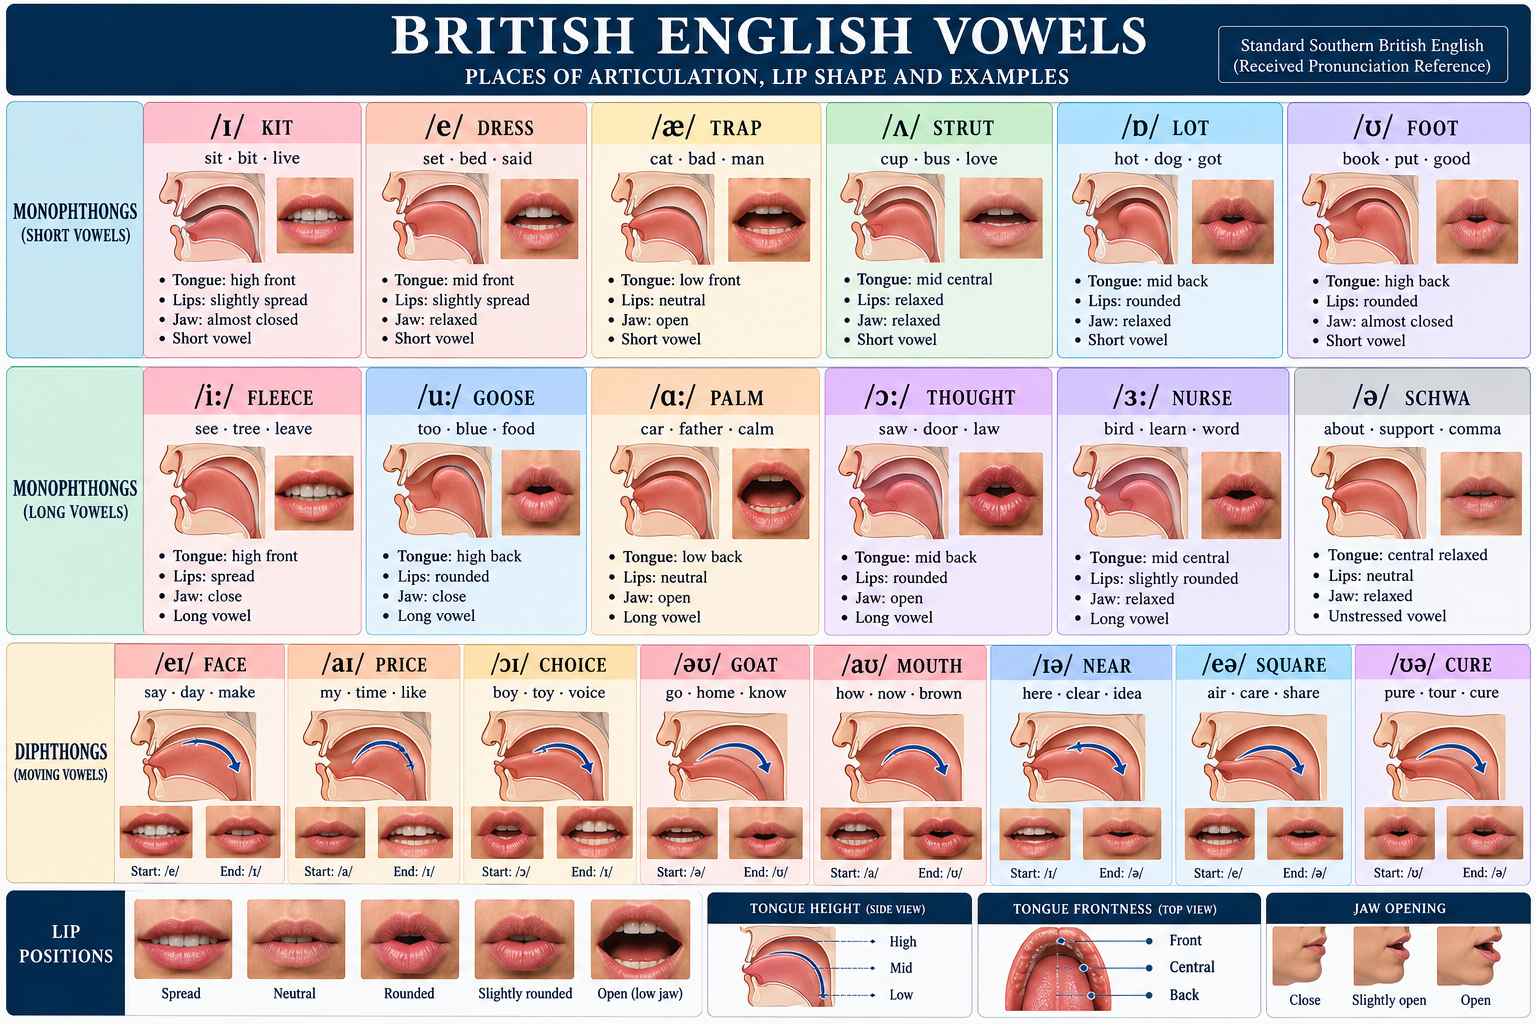
\includegraphics[width=1\linewidth]{images/all-in-one-british-vowels.png}
    \caption{British English vowels postures of the vocal organs}
    \label{fig:british-english-vowels}
\end{figure}

\noindent\textbf{Target accent:} contemporary Standard Southern British English (SSBE), with traditional Received Pronunciation (RP) comparisons.\par
\noindent\textbf{Suggested duration:} 6--8 weeks within a two-hour daily training programme. This is a planning estimate, not a guaranteed proficiency timeline.\par
\noindent\textbf{Prerequisites:} basic understanding of syllables and familiarity with dictionary entries.\par
\section{Learning outcomes}
By the end of this chapter, the learner should be able to (i) recognise the major SSBE vowel categories in isolated and connected speech; (ii) describe and reproduce their articulatory targets; (iii) distinguish important minimal pairs; (iv) recognise weak forms and schwa; (v) interpret broad IPA transcription; and (vi) monitor vowel accuracy during academic and professional communication.
\section{How to use this chapter}
Each vowel laboratory follows the sequence \emph{listen, discriminate, position, produce, contrast, read, record, review}. Do not increase speaking speed until the contrast is reliably audible and producible. Audio prompts are marked as resources and must be recorded or sourced before listening-only tests are administered.
\res{AUD-000}{Master accent reference recording}{One adult SSBE speaker and a second comparison speaker; isolated vowels, lexical-set keywords, slow and natural-speed phrases; lossless WAV and accessible MP3.}
\section{Diagnostic baseline}
Record a 60-second introduction, read the passage below, and pronounce the word pairs \emph{sheep--ship, bed--bad, cut--cart, full--fool, cot--caught, late--light}. Save both unedited audio and a brief self-assessment. The recording is a baseline rather than a pass/fail test.
\task{Baseline reading}{``This week I need to explain the results of our latest experiment. We checked the data, compared the figures and discussed which changes would improve the system. I would like to present a clear summary at the next meeting.'' Record once at normal speed, then annotate the vowels you find difficult.}
\res{REC-001}{Baseline recording form}{Date, microphone conditions, reading time, confidence, target words, observed problems, and link to audio file.}
\section{The physiology of vowels}
Vowels are typically voiced speech sounds produced without a complete closure or a turbulent constriction in the vocal tract. Vowel quality depends strongly on tongue position, lip posture, jaw opening and the resulting vocal-tract resonances. The traditional vowel quadrilateral is an articulatory map, not a literal photograph of the tongue.
\subsection{Height, backness and lip rounding}
\emph{Height} describes the vertical position of the tongue body; \emph{backness} describes its front-to-back position. Rounded lips can lengthen the effective vocal tract and change resonance. Jaw movement and tongue movement are related but not identical.
\res{FIG-001}{Sagittal vocal-tract anatomy}{Label lips, jaw, tongue tip, blade, body and root, hard palate, soft palate, pharynx, and larynx; vector PDF preferred.}
\res{FIG-002}{IPA vowel quadrilateral}{High/mid/low and front/central/back axes, with schematic SSBE vowel locations; include note about speaker variation.}
\res{FIG-003}{Lip and jaw posture plate}{Photographic or schematic front views for spread, neutral, rounded and open positions; matched scale and neutral lighting.}
\subsection{Length, stress and context}
The colon-like length mark \texttt{ː} distinguishes conventional broad transcriptions such as \ipa{iː} from \ipa{ɪ}. Actual duration also varies with stress, speech rate and following consonants. In particular, a vowel is commonly shorter before a fortis consonant than before a lenis consonant: compare \emph{seat} and \emph{seed}. Never rely on duration alone to identify an English vowel.
\res{FIG-004}{Pre-fortis clipping timeline}{Compare the same vowel in seat/seed and beat/bead, with measured examples and speaker metadata; do not fabricate durations.}
\subsection{A note on notation and accent variation}
Broad transcriptions are pedagogical approximations. Modern SSBE may use a fronter GOOSE vowel, variable GOAT onsets, and monophthongal pronunciations in words historically transcribed with centring diphthongs. The traditional RP CURE category \ipa{ʊə} is often merged with THOUGHT \ipa{ɔː} in common words such as \emph{sure}; NEAR and SQUARE may also vary. Learn the reference model, then recognise variants without treating every difference as an error.
\section{The vowel inventory}
\begin{longtable}{lll p{0.38\linewidth}}
\toprule Class & Lexical set & Broad IPA & Keyword and note\\\midrule\endhead
Short & KIT & \ipa{ɪ} & kit\\
Short & DRESS & \ipa{e} & dress\\
Short & TRAP & \ipa{æ} & trap\\
Short & STRUT & \ipa{ʌ} & strut\\
Short & LOT & \ipa{ɒ} & lot\\
Short & FOOT & \ipa{ʊ} & foot\\
Long & FLEECE & \ipa{iː} & fleece\\
Long & GOOSE & \ipa{uː} & goose\\
Long & PALM & \ipa{ɑː} & palm\\
Long & THOUGHT & \ipa{ɔː} & thought\\
Long & NURSE & \ipa{ɜː} & nurse\\
Weak & commA & \ipa{ə} & about, comma (unstressed)\\
Diphthong & FACE & \ipa{eɪ} & face\\
Diphthong & PRICE & \ipa{aɪ} & price\\
Diphthong & CHOICE & \ipa{ɔɪ} & choice\\
Diphthong & GOAT & \ipa{əʊ} & goat (traditional broad SSBE)\\
Diphthong & MOUTH & \ipa{aʊ} & mouth\\
Variable centring & NEAR & \ipa{ɪə} & near; modern variants exist\\
Variable centring & SQUARE & \ipa{eə} & square; modern variants exist\\
Variable centring & CURE & \ipa{ʊə} & cure; limited and variable in modern SSBE\\
\bottomrule
\end{longtable}
\res{FIG-005}{Master vowel chart poster}{All lexical sets, IPA, example words, colour-coded categories, and centring-diphthong variation warning; A3 printable PDF and SVG.}

\section{Preparatory articulation gym}

\begin{enumerate}[label=\arabic*.]
\item \textbf{Jaw release (60 s):} alternate relaxed closed-mouth posture and comfortable opening without forcing the joint.
\item \textbf{Lip alternation (60 s):} move gently between spread, neutral and rounded lips without voicing.
\item \textbf{Tongue awareness (90 s):} alternate a high-front and a high-back tongue-body position; avoid pressing against the palate.
\item \textbf{Sustained voicing (60 s):} sustain a comfortable vowel for several seconds, keeping the pitch and loudness stable.
\item \textbf{Vowel-space ladder (3 min):} repeat \ipa{iː}--\ipa{ɪ}--\ipa{e}--\ipa{æ}--\ipa{ɑː}, slowly and without inserting consonants.
\item \textbf{Rounding ladder (3 min):} contrast \ipa{uː}, \ipa{ʊ}, \ipa{ɔː}, \ipa{ɒ}; use a mirror to notice the lips.
\item \textbf{Silent-to-voiced transfer (2 min):} form the target mouth shape silently, then voice it without shifting position.
\end{enumerate}

Stop any movement that causes pain or strain; exaggerated articulation is a temporary training aid, not a speaking goal.
\res{VID-001}{Articulatory warm-up demonstration}{Close-up front and side videos with slow motion, subtitles and accessible verbal instructions.}
\task{Preparation checklist}{Mark each as comfortable / uncertain / difficult: lip rounding, jaw opening, high-front tongue, back-vowel posture, steady voicing, and silent-to-voiced transfer. Repeat uncertain movements before the next laboratory.}

\section{KIT: \ipa{ɪ}}
\label{sec:vowel-01}

\begin{figure}[H]
    \centering
    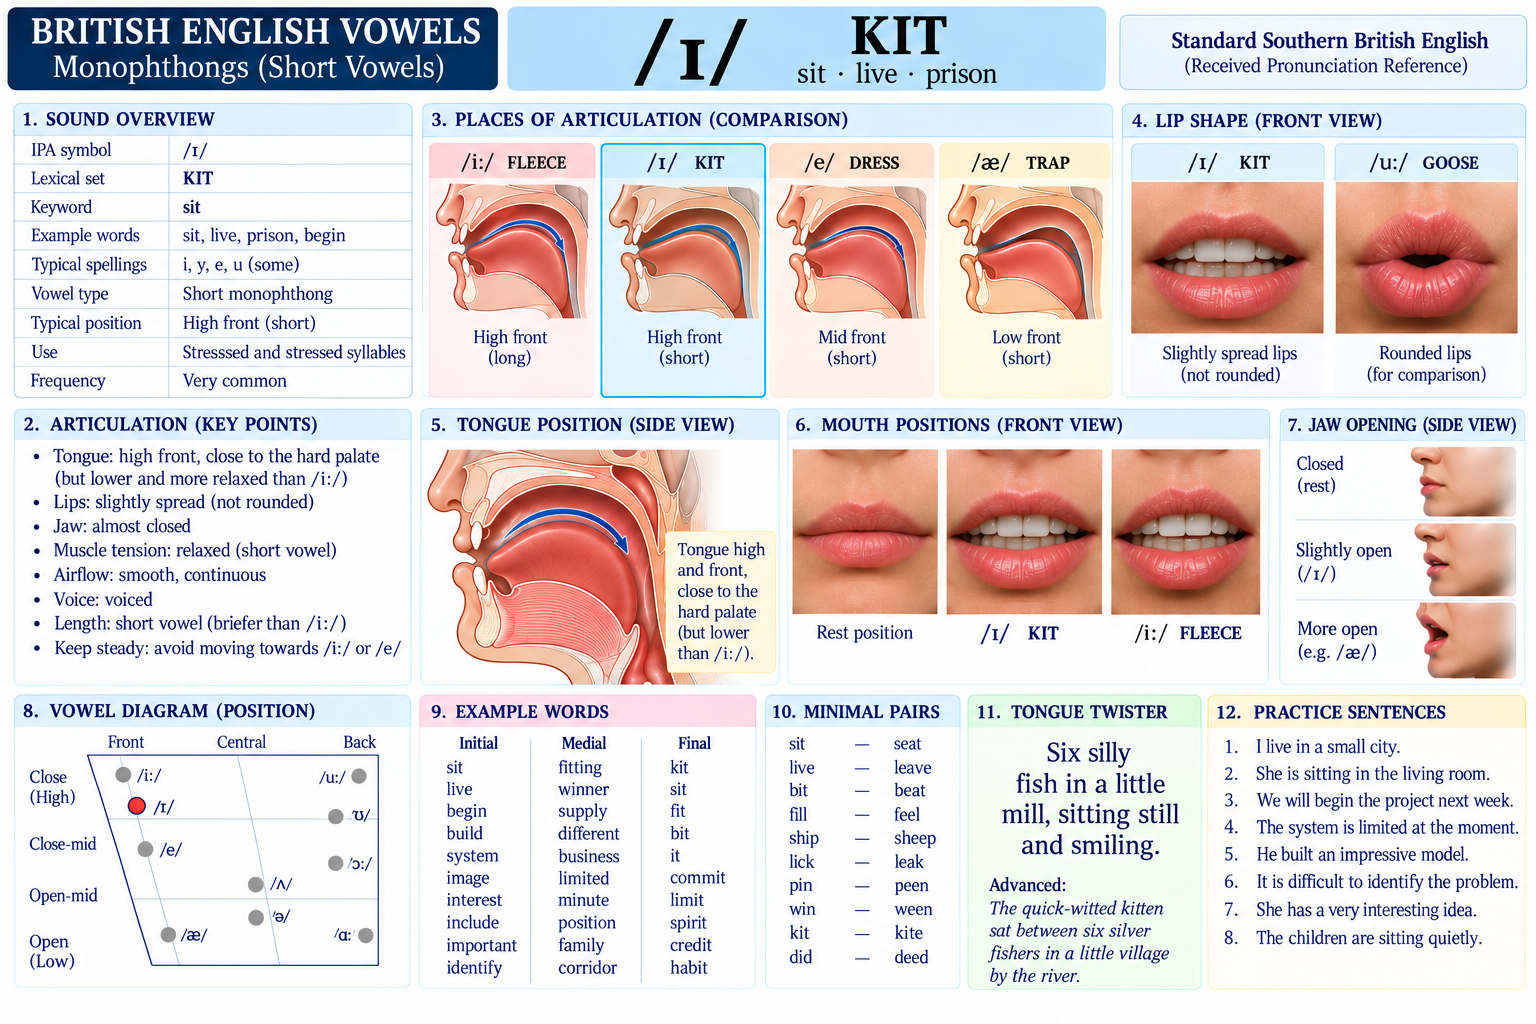
\includegraphics[width=1\linewidth]{images/vowel-ii.png}
    \caption{Enter Caption}
    \label{fig:placeholder}
\end{figure}
\textbf{Lexical anchor:} kit. \textbf{Core examples:} sit, ship, live, rich, fill.\par
\textbf{Articulatory target:} Keep the tongue near-high and front; the vowel is typically more central and lax than FLEECE. Observe tongue-body placement, lip posture and jaw aperture; compare your recording with the reference speaker rather than using spelling as a guide.
\res{FIG-101}{KIT articulation plate}{Front and sagittal views, highlighted tongue target and lips, vowel-map dot, and comparison with nearest category; SVG and PDF.}
\res{AUD-101}{KIT native-speaker model}{Isolated target (three repetitions), each example word (slow/natural), minimal-pair contrasts, phrase, sentence and tongue twister; WAV/MP3, transcript and speaker metadata.}
\subsection{Perception and discrimination}
\task{Hear the difference}{Use the companion audio. For ten randomised trials, identify the target vowel or the contrasting vowel. Write your choice and confidence (1--5). Include at least two repeated items to check consistency. No answer can be scored until the audio stimulus list is supplied.}
\res{LST-101}{KIT discrimination test}{Ten balanced, randomised tokens with answer key, trial order, lexical context and no visible words during listening.}
\subsection{Production ladder}
\begin{enumerate}[label=\arabic*.]
\item Sustain \ipa{ɪ} gently three times; compare with the model.
\item Say each core example in isolation, then embed it in ``I said \emph{[word]} clearly.''
\item Practise the contrasts: sheep--ship; leave--live; feel--fill.
\item Repeat each contrast at slow, conversational and presentation speeds.
\item Record the sentence below and listen for target-vowel consistency.
\end{enumerate}
\textbf{Controlled sentence:} Six little ships slipped into the mist.
\subsection{Tongue-twister laboratory}
Say the controlled sentence three times accurately, then twice at natural speed. Mark any vowel that shifts category. Speed is secondary to intelligibility.
\subsection{Reading and transfer}
\task{Mini-reading and spontaneous transfer}{Read the following original prompt aloud, then speak for 30--45 seconds without a script: ``Explain a recent decision, the evidence behind it, and the next action.'' Insert at least three words from this vowel laboratory. Underline them in your transcript and review their pronunciation.}
\res{TXT-101}{KIT graded reading}{A 100--150-word original passage with 12--20 instances of the target vowel, marked and unmarked versions, vocabulary glosses and comprehension questions.}
\res{REC-101}{KIT recording worksheet}{Word checklist, contrast accuracy, vowel stability, speaking-rate notes, self-correction and tutor feedback.}

\section{DRESS: \ipa{e}}
\label{sec:vowel-02}

\begin{figure}[H]
    \centering
    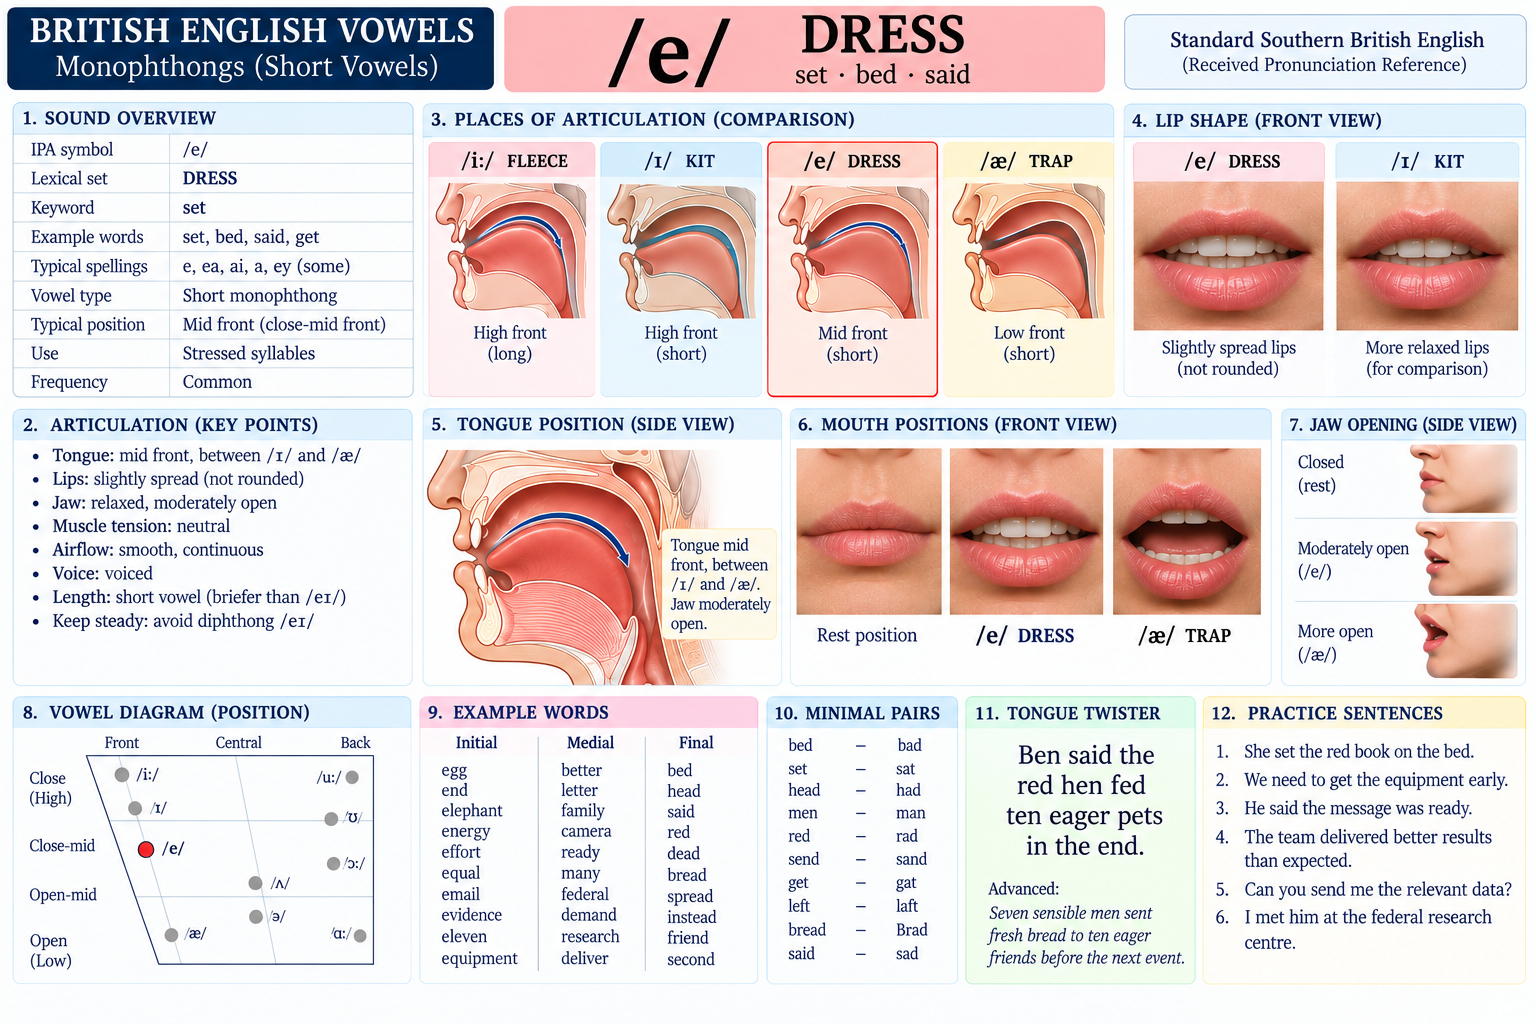
\includegraphics[width=1\linewidth]{images/vowel-e.png}
    \caption{Vowel \ipa{e} construction}
    \label{fig:placeholder}
\end{figure}

\textbf{Lexical anchor:} dress. \textbf{Core examples:} bed, head, said, ten, send.\par
\textbf{Articulatory target:} Use a mid-front tongue position with relatively neutral lips. Observe tongue-body placement, lip posture and jaw aperture; compare your recording with the reference speaker rather than using spelling as a guide.
\res{FIG-102}{DRESS articulation plate}{Front and sagittal views, highlighted tongue target and lips, vowel-map dot, and comparison with nearest category; SVG and PDF.}
\res{AUD-102}{DRESS native-speaker model}{Isolated target (three repetitions), each example word (slow/natural), minimal-pair contrasts, phrase, sentence and tongue twister; WAV/MP3, transcript and speaker metadata.}
\subsection{Perception and discrimination}
\task{Hear the difference}{Use the companion audio. For ten randomised trials, identify the target vowel or the contrasting vowel. Write your choice and confidence (1--5). Include at least two repeated items to check consistency. No answer can be scored until the audio stimulus list is supplied.}
\res{LST-102}{DRESS discrimination test}{Ten balanced, randomised tokens with answer key, trial order, lexical context and no visible words during listening.}
\subsection{Production ladder}
\begin{enumerate}[label=\arabic*.]
\item Sustain \ipa{e} gently three times; compare with the model.
\item Say each core example in isolation, then embed it in ``I said \emph{[word]} clearly.''
\item Practise the contrasts: bed--bad; men--man; pen--pan.
\item Repeat each contrast at slow, conversational and presentation speeds.
\item Record the sentence below and listen for target-vowel consistency.
\end{enumerate}
\textbf{Controlled sentence:} Ten clever friends checked the red pens.
\subsection{Tongue-twister laboratory}
Say the controlled sentence three times accurately, then twice at natural speed. Mark any vowel that shifts category. Speed is secondary to intelligibility.
\subsection{Reading and transfer}
\task{Mini-reading and spontaneous transfer}{Read the following original prompt aloud, then speak for 30--45 seconds without a script: ``Explain a recent decision, the evidence behind it, and the next action.'' Insert at least three words from this vowel laboratory. Underline them in your transcript and review their pronunciation.}
\res{TXT-102}{DRESS graded reading}{A 100--150-word original passage with 12--20 instances of the target vowel, marked and unmarked versions, vocabulary glosses and comprehension questions.}
\res{REC-102}{DRESS recording worksheet}{Word checklist, contrast accuracy, vowel stability, speaking-rate notes, self-correction and tutor feedback.}

\section{TRAP: \ipa{æ}}
\label{sec:vowel-03}

\begin{figure}[H]
    \centering
    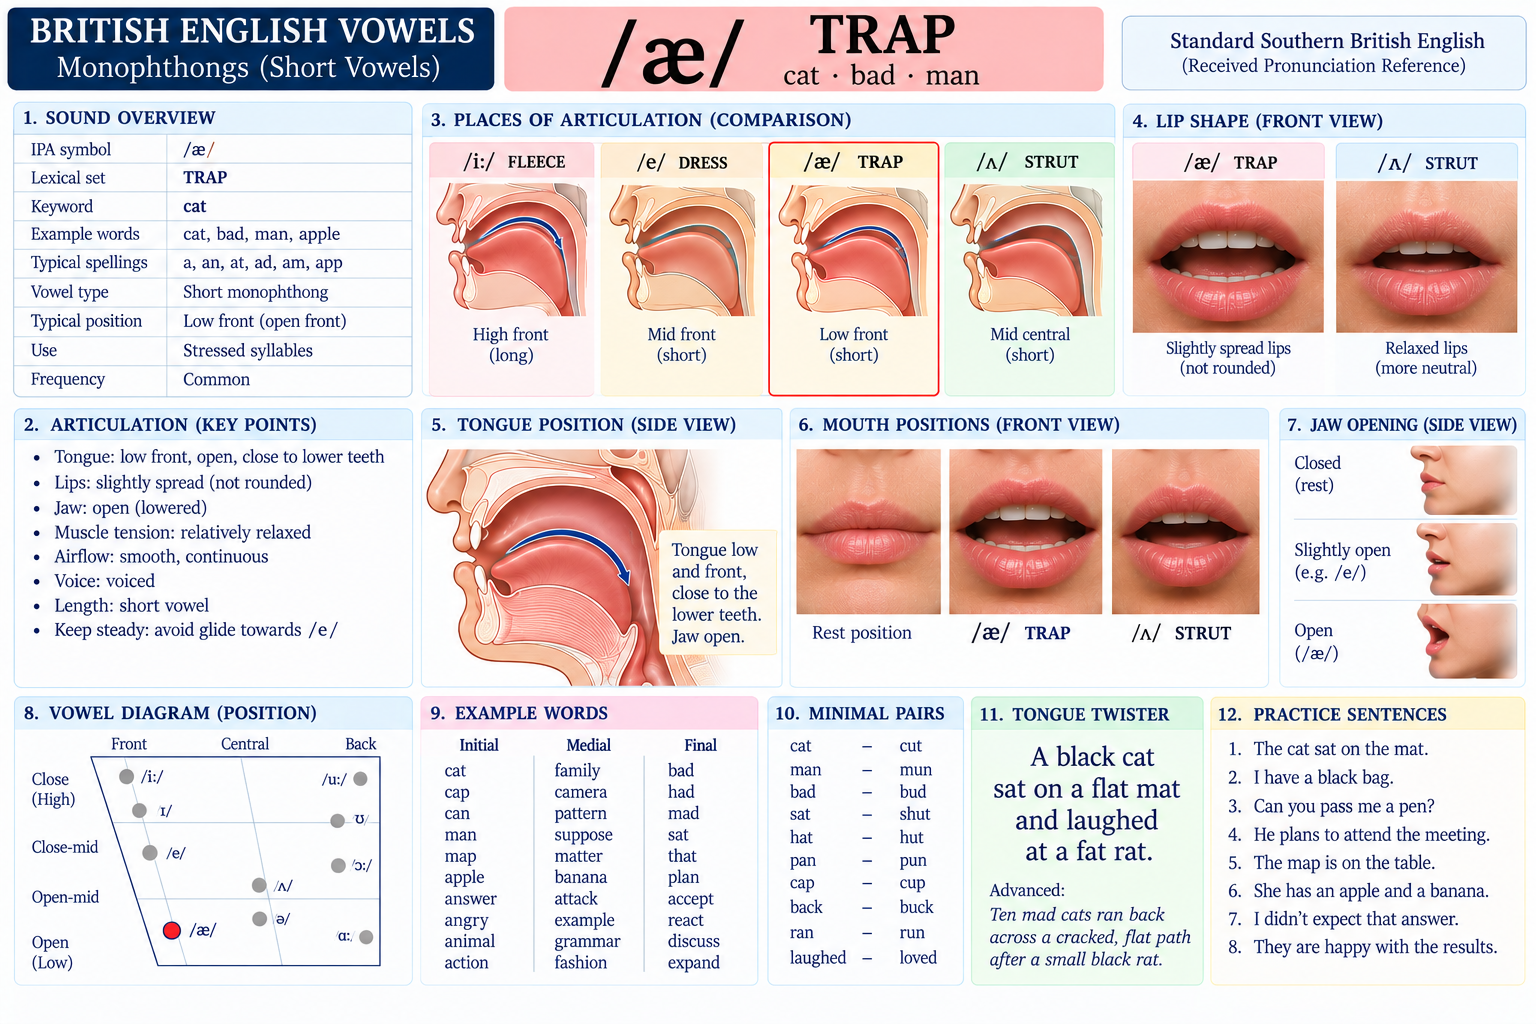
\includegraphics[width=1\linewidth]{images/vowel-ae.png}
    \caption{Vowel \ipa{æ} construction}
    \label{fig:placeholder}
\end{figure}

\textbf{Lexical anchor:} trap. \textbf{Core examples:} cat, bad, map, plan, match.\par
\textbf{Articulatory target:} Lower the front tongue and open the jaw comfortably; avoid replacing it with Spanish /a/. Observe tongue-body placement, lip posture and jaw aperture; compare your recording with the reference speaker rather than using spelling as a guide.
\res{FIG-103}{TRAP articulation plate}{Front and sagittal views, highlighted tongue target and lips, vowel-map dot, and comparison with nearest category; SVG and PDF.}
\res{AUD-103}{TRAP native-speaker model}{Isolated target (three repetitions), each example word (slow/natural), minimal-pair contrasts, phrase, sentence and tongue twister; WAV/MP3, transcript and speaker metadata.}
\subsection{Perception and discrimination}
\task{Hear the difference}{Use the companion audio. For ten randomised trials, identify the target vowel or the contrasting vowel. Write your choice and confidence (1--5). Include at least two repeated items to check consistency. No answer can be scored until the audio stimulus list is supplied.}
\res{LST-103}{TRAP discrimination test}{Ten balanced, randomised tokens with answer key, trial order, lexical context and no visible words during listening.}
\subsection{Production ladder}
\begin{enumerate}[label=\arabic*.]
\item Sustain \ipa{æ} gently three times; compare with the model.
\item Say each core example in isolation, then embed it in ``I said \emph{[word]} clearly.''
\item Practise the contrasts: bad--bed; man--men; hat--hut.
\item Repeat each contrast at slow, conversational and presentation speeds.
\item Record the sentence below and listen for target-vowel consistency.
\end{enumerate}
\textbf{Controlled sentence:} A happy manager mapped the plan.
\subsection{Tongue-twister laboratory}
Say the controlled sentence three times accurately, then twice at natural speed. Mark any vowel that shifts category. Speed is secondary to intelligibility.
\subsection{Reading and transfer}
\task{Mini-reading and spontaneous transfer}{Read the following original prompt aloud, then speak for 30--45 seconds without a script: ``Explain a recent decision, the evidence behind it, and the next action.'' Insert at least three words from this vowel laboratory. Underline them in your transcript and review their pronunciation.}

\res{TXT-103}{TRAP graded reading}{A 100--150-word original passage with 12--20 instances of the target vowel, marked and unmarked versions, vocabulary glosses and comprehension questions.}

\res{REC-103}{TRAP recording worksheet}{Word checklist, contrast accuracy, vowel stability, speaking-rate notes, self-correction and tutor feedback.}

\section{STRUT: \ipa{ʌ}}
\label{sec:vowel-04}

\begin{figure}[H]
    \centering
    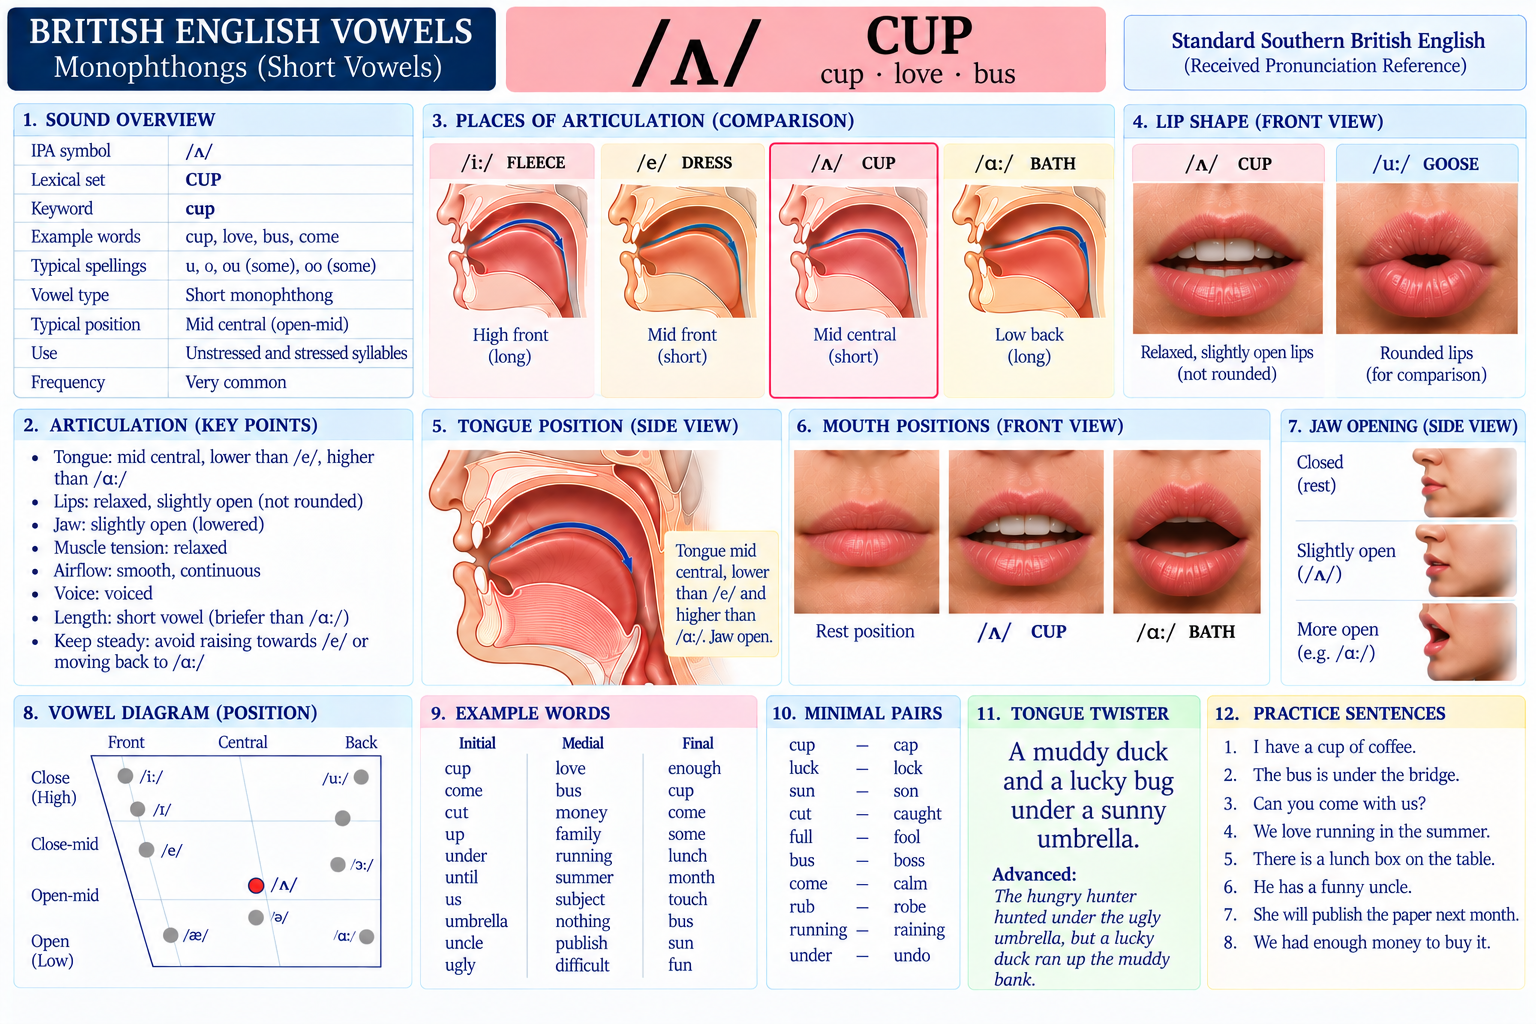
\includegraphics[width=1\linewidth]{images/vowel-u.png}
    \caption{Vowel \ipa{ʌ} construction}
    \label{fig:placeholder}
\end{figure}


\textbf{Lexical anchor:} strut. \textbf{Core examples:} cup, luck, much, money, sun.\par
\textbf{Articulatory target:} Use a central-to-back open-mid target, generally with unrounded lips. Observe tongue-body placement, lip posture and jaw aperture; compare your recording with the reference speaker rather than using spelling as a guide.
\res{FIG-104}{STRUT articulation plate}{Front and sagittal views, highlighted tongue target and lips, vowel-map dot, and comparison with nearest category; SVG and PDF.}
\res{AUD-104}{STRUT native-speaker model}{Isolated target (three repetitions), each example word (slow/natural), minimal-pair contrasts, phrase, sentence and tongue twister; WAV/MP3, transcript and speaker metadata.}
\subsection{Perception and discrimination}
\task{Hear the difference}{Use the companion audio. For ten randomised trials, identify the target vowel or the contrasting vowel. Write your choice and confidence (1--5). Include at least two repeated items to check consistency. No answer can be scored until the audio stimulus list is supplied.}
\res{LST-104}{STRUT discrimination test}{Ten balanced, randomised tokens with answer key, trial order, lexical context and no visible words during listening.}
\subsection{Production ladder}
\begin{enumerate}[label=\arabic*.]
\item Sustain \ipa{ʌ} gently three times; compare with the model.
\item Say each core example in isolation, then embed it in ``I said \emph{[word]} clearly.''
\item Practise the contrasts: cut--cart; luck--lock; hut--hat.
\item Repeat each contrast at slow, conversational and presentation speeds.
\item Record the sentence below and listen for target-vowel consistency.
\end{enumerate}
\textbf{Controlled sentence:} A young consultant discussed the budget.
\subsection{Tongue-twister laboratory}
Say the controlled sentence three times accurately, then twice at natural speed. Mark any vowel that shifts category. Speed is secondary to intelligibility.
\subsection{Reading and transfer}
\task{Mini-reading and spontaneous transfer}{Read the following original prompt aloud, then speak for 30--45 seconds without a script: ``Explain a recent decision, the evidence behind it, and the next action.'' Insert at least three words from this vowel laboratory. Underline them in your transcript and review their pronunciation.}
\res{TXT-104}{STRUT graded reading}{A 100--150-word original passage with 12--20 instances of the target vowel, marked and unmarked versions, vocabulary glosses and comprehension questions.}
\res{REC-104}{STRUT recording worksheet}{Word checklist, contrast accuracy, vowel stability, speaking-rate notes, self-correction and tutor feedback.}

\section{LOT: \ipa{ɒ}}
\label{sec:vowel-05}

\begin{figure}[H]
    \centering
    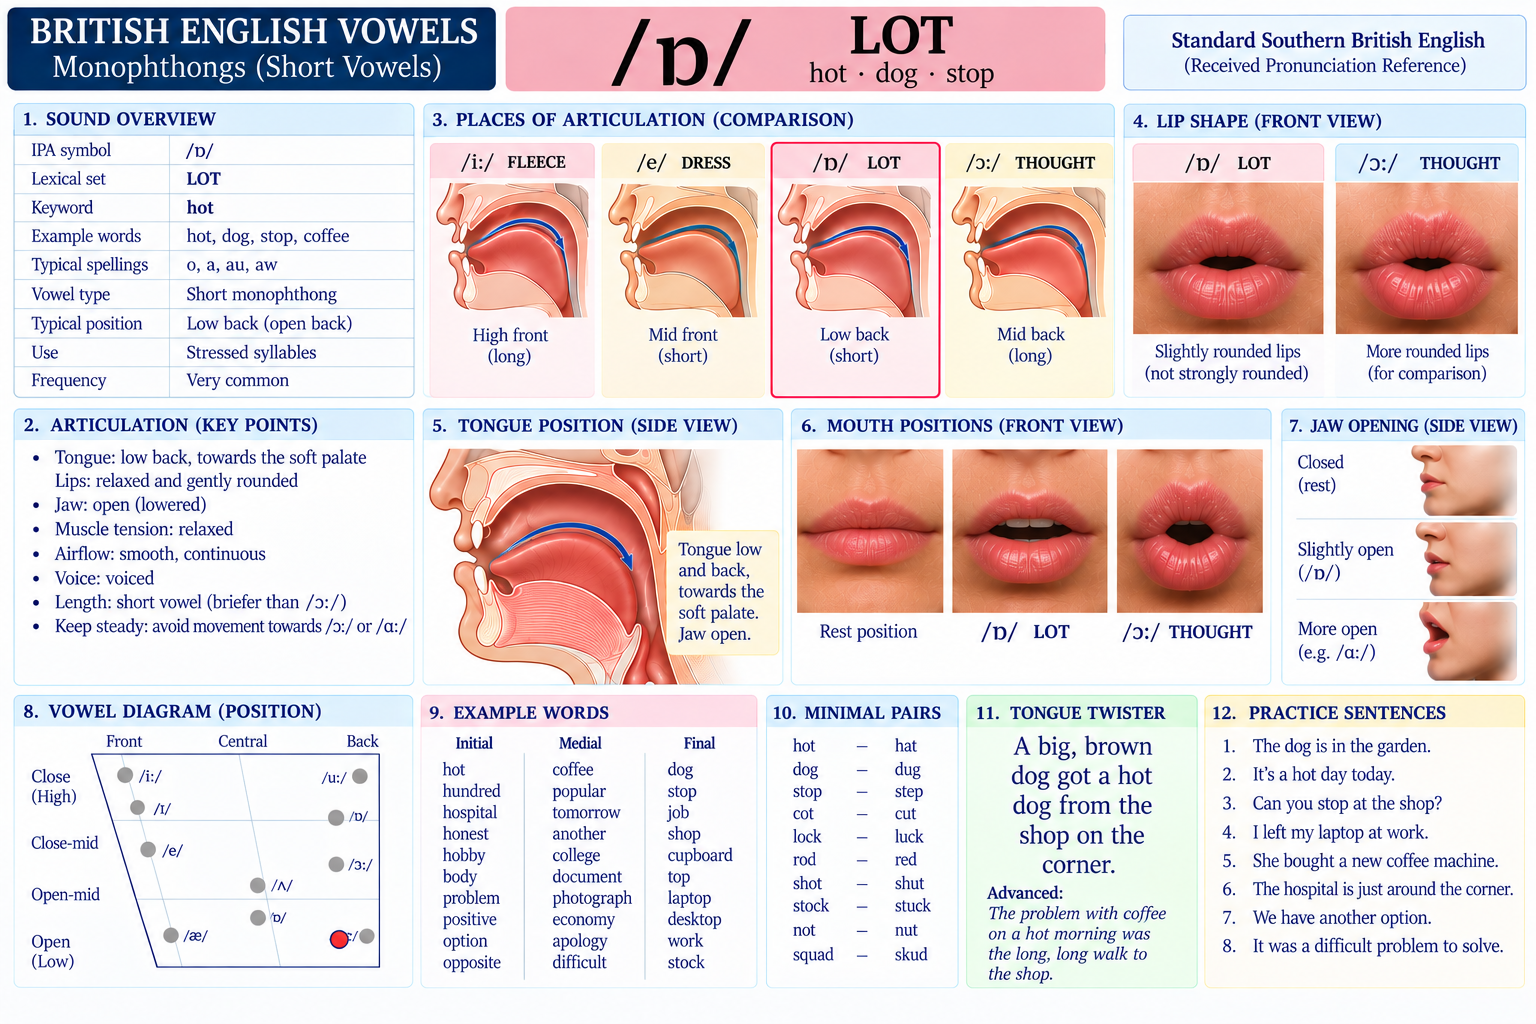
\includegraphics[width=1\linewidth]{images/vowel-a.png}
    \caption{Vowel \ipa{ɒ} construction}
    \label{fig:placeholder}
\end{figure}

\textbf{Lexical anchor:} lot. \textbf{Core examples:} lot, stop, clock, shop, problem.\par
\textbf{Articulatory target:} Aim for a relatively open, back and rounded vowel in the target accent. Observe tongue-body placement, lip posture and jaw aperture; compare your recording with the reference speaker rather than using spelling as a guide.
\res{FIG-105}{LOT articulation plate}{Front and sagittal views, highlighted tongue target and lips, vowel-map dot, and comparison with nearest category; SVG and PDF.}
\res{AUD-105}{LOT native-speaker model}{Isolated target (three repetitions), each example word (slow/natural), minimal-pair contrasts, phrase, sentence and tongue twister; WAV/MP3, transcript and speaker metadata.}
\subsection{Perception and discrimination}
\task{Hear the difference}{Use the companion audio. For ten randomised trials, identify the target vowel or the contrasting vowel. Write your choice and confidence (1--5). Include at least two repeated items to check consistency. No answer can be scored until the audio stimulus list is supplied.}
\res{LST-105}{LOT discrimination test}{Ten balanced, randomised tokens with answer key, trial order, lexical context and no visible words during listening.}
\subsection{Production ladder}
\begin{enumerate}[label=\arabic*.]
\item Sustain \ipa{ɒ} gently three times; compare with the model.
\item Say each core example in isolation, then embed it in ``I said \emph{[word]} clearly.''
\item Practise the contrasts: cot--caught; stock--stalk; not--nought.
\item Repeat each contrast at slow, conversational and presentation speeds.
\item Record the sentence below and listen for target-vowel consistency.
\end{enumerate}
\textbf{Controlled sentence:} The project stopped at the wrong clock.
\subsection{Tongue-twister laboratory}
Say the controlled sentence three times accurately, then twice at natural speed. Mark any vowel that shifts category. Speed is secondary to intelligibility.
\subsection{Reading and transfer}
\task{Mini-reading and spontaneous transfer}{Read the following original prompt aloud, then speak for 30--45 seconds without a script: ``Explain a recent decision, the evidence behind it, and the next action.'' Insert at least three words from this vowel laboratory. Underline them in your transcript and review their pronunciation.}
\res{TXT-105}{LOT graded reading}{A 100--150-word original passage with 12--20 instances of the target vowel, marked and unmarked versions, vocabulary glosses and comprehension questions.}
\res{REC-105}{LOT recording worksheet}{Word checklist, contrast accuracy, vowel stability, speaking-rate notes, self-correction and tutor feedback.}

\section{FOOT: \ipa{ʊ}}
\label{sec:vowel-06}

\begin{figure}[H]
    \centering
    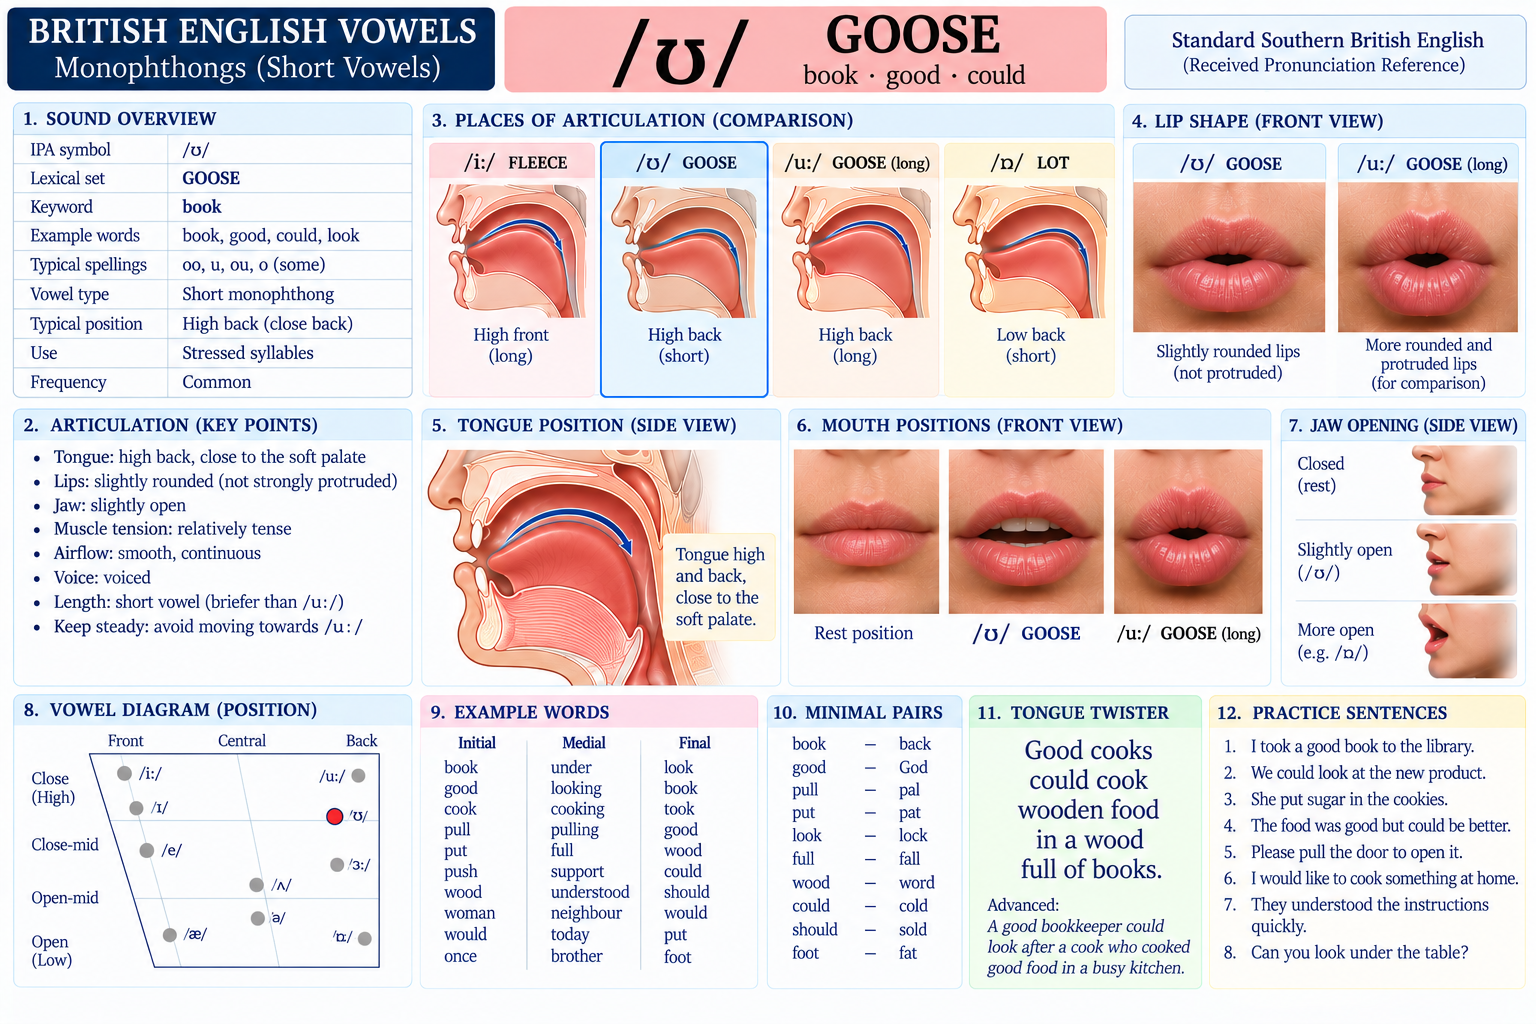
\includegraphics[width=1\linewidth]{images/vowel-uu.png}
    \caption{Vowel \ipa{ʊ} construction}
    \label{fig:placeholder}
\end{figure}

\textbf{Lexical anchor:} foot. \textbf{Core examples:} put, good, book, could, full.\par
\textbf{Articulatory target:} Use a near-high, back-to-central rounded target, distinct from GOOSE. Observe tongue-body placement, lip posture and jaw aperture; compare your recording with the reference speaker rather than using spelling as a guide.
\res{FIG-106}{FOOT articulation plate}{Front and sagittal views, highlighted tongue target and lips, vowel-map dot, and comparison with nearest category; SVG and PDF.}
\res{AUD-106}{FOOT native-speaker model}{Isolated target (three repetitions), each example word (slow/natural), minimal-pair contrasts, phrase, sentence and tongue twister; WAV/MP3, transcript and speaker metadata.}
\subsection{Perception and discrimination}
\task{Hear the difference}{Use the companion audio. For ten randomised trials, identify the target vowel or the contrasting vowel. Write your choice and confidence (1--5). Include at least two repeated items to check consistency. No answer can be scored until the audio stimulus list is supplied.}
\res{LST-106}{FOOT discrimination test}{Ten balanced, randomised tokens with answer key, trial order, lexical context and no visible words during listening.}
\subsection{Production ladder}
\begin{enumerate}[label=\arabic*.]
\item Sustain \ipa{ʊ} gently three times; compare with the model.
\item Say each core example in isolation, then embed it in ``I said \emph{[word]} clearly.''
\item Practise the contrasts: full--fool; pull--pool; look--Luke.
\item Repeat each contrast at slow, conversational and presentation speeds.
\item Record the sentence below and listen for target-vowel consistency.
\end{enumerate}
\textbf{Controlled sentence:} The good cook took a full book.
\subsection{Tongue-twister laboratory}
Say the controlled sentence three times accurately, then twice at natural speed. Mark any vowel that shifts category. Speed is secondary to intelligibility.
\subsection{Reading and transfer}
\task{Mini-reading and spontaneous transfer}{Read the following original prompt aloud, then speak for 30--45 seconds without a script: ``Explain a recent decision, the evidence behind it, and the next action.'' Insert at least three words from this vowel laboratory. Underline them in your transcript and review their pronunciation.}
\res{TXT-106}{FOOT graded reading}{A 100--150-word original passage with 12--20 instances of the target vowel, marked and unmarked versions, vocabulary glosses and comprehension questions.}
\res{REC-106}{FOOT recording worksheet}{Word checklist, contrast accuracy, vowel stability, speaking-rate notes, self-correction and tutor feedback.}

\section{FLEECE: \ipa{iː}}
\label{sec:vowel-07}
\textbf{Lexical anchor:} fleece. \textbf{Core examples:} see, meet, team, leave, machine.\par
\textbf{Articulatory target:} Use a high-front vowel with a stable quality; avoid a strong closing glide. Observe tongue-body placement, lip posture and jaw aperture; compare your recording with the reference speaker rather than using spelling as a guide.
\res{FIG-107}{FLEECE articulation plate}{Front and sagittal views, highlighted tongue target and lips, vowel-map dot, and comparison with nearest category; SVG and PDF.}
\res{AUD-107}{FLEECE native-speaker model}{Isolated target (three repetitions), each example word (slow/natural), minimal-pair contrasts, phrase, sentence and tongue twister; WAV/MP3, transcript and speaker metadata.}
\subsection{Perception and discrimination}
\task{Hear the difference}{Use the companion audio. For ten randomised trials, identify the target vowel or the contrasting vowel. Write your choice and confidence (1--5). Include at least two repeated items to check consistency. No answer can be scored until the audio stimulus list is supplied.}
\res{LST-107}{FLEECE discrimination test}{Ten balanced, randomised tokens with answer key, trial order, lexical context and no visible words during listening.}
\subsection{Production ladder}
\begin{enumerate}[label=\arabic*.]
\item Sustain \ipa{iː} gently three times; compare with the model.
\item Say each core example in isolation, then embed it in ``I said \emph{[word]} clearly.''
\item Practise the contrasts: sheep--ship; seat--sit; reach--rich.
\item Repeat each contrast at slow, conversational and presentation speeds.
\item Record the sentence below and listen for target-vowel consistency.
\end{enumerate}
\textbf{Controlled sentence:} Three keen researchers reviewed the scheme.
\subsection{Tongue-twister laboratory}
Say the controlled sentence three times accurately, then twice at natural speed. Mark any vowel that shifts category. Speed is secondary to intelligibility.
\subsection{Reading and transfer}
\task{Mini-reading and spontaneous transfer}{Read the following original prompt aloud, then speak for 30--45 seconds without a script: ``Explain a recent decision, the evidence behind it, and the next action.'' Insert at least three words from this vowel laboratory. Underline them in your transcript and review their pronunciation.}
\res{TXT-107}{FLEECE graded reading}{A 100--150-word original passage with 12--20 instances of the target vowel, marked and unmarked versions, vocabulary glosses and comprehension questions.}
\res{REC-107}{FLEECE recording worksheet}{Word checklist, contrast accuracy, vowel stability, speaking-rate notes, self-correction and tutor feedback.}

\section{GOOSE: \ipa{uː}}
\label{sec:vowel-08}
\textbf{Lexical anchor:} goose. \textbf{Core examples:} food, blue, move, group, student.\par
\textbf{Articulatory target:} Use a high vowel with rounding; many modern speakers have a noticeably fronted tongue position. Observe tongue-body placement, lip posture and jaw aperture; compare your recording with the reference speaker rather than using spelling as a guide.
\res{FIG-108}{GOOSE articulation plate}{Front and sagittal views, highlighted tongue target and lips, vowel-map dot, and comparison with nearest category; SVG and PDF.}
\res{AUD-108}{GOOSE native-speaker model}{Isolated target (three repetitions), each example word (slow/natural), minimal-pair contrasts, phrase, sentence and tongue twister; WAV/MP3, transcript and speaker metadata.}
\subsection{Perception and discrimination}
\task{Hear the difference}{Use the companion audio. For ten randomised trials, identify the target vowel or the contrasting vowel. Write your choice and confidence (1--5). Include at least two repeated items to check consistency. No answer can be scored until the audio stimulus list is supplied.}
\res{LST-108}{GOOSE discrimination test}{Ten balanced, randomised tokens with answer key, trial order, lexical context and no visible words during listening.}
\subsection{Production ladder}
\begin{enumerate}[label=\arabic*.]
\item Sustain \ipa{uː} gently three times; compare with the model.
\item Say each core example in isolation, then embed it in ``I said \emph{[word]} clearly.''
\item Practise the contrasts: fool--full; pool--pull; Luke--look.
\item Repeat each contrast at slow, conversational and presentation speeds.
\item Record the sentence below and listen for target-vowel consistency.
\end{enumerate}
\textbf{Controlled sentence:} Two students moved the blue tools.
\subsection{Tongue-twister laboratory}
Say the controlled sentence three times accurately, then twice at natural speed. Mark any vowel that shifts category. Speed is secondary to intelligibility.
\subsection{Reading and transfer}
\task{Mini-reading and spontaneous transfer}{Read the following original prompt aloud, then speak for 30--45 seconds without a script: ``Explain a recent decision, the evidence behind it, and the next action.'' Insert at least three words from this vowel laboratory. Underline them in your transcript and review their pronunciation.}
\res{TXT-108}{GOOSE graded reading}{A 100--150-word original passage with 12--20 instances of the target vowel, marked and unmarked versions, vocabulary glosses and comprehension questions.}
\res{REC-108}{GOOSE recording worksheet}{Word checklist, contrast accuracy, vowel stability, speaking-rate notes, self-correction and tutor feedback.}

\section{PALM: \ipa{ɑː}}
\label{sec:vowel-09}
\textbf{Lexical anchor:} palm. \textbf{Core examples:} father, calm, start, hard, class.\par
\textbf{Articulatory target:} Use an open back unrounded target; note non-rhotic spelling in start and hard. Observe tongue-body placement, lip posture and jaw aperture; compare your recording with the reference speaker rather than using spelling as a guide.
\res{FIG-109}{PALM articulation plate}{Front and sagittal views, highlighted tongue target and lips, vowel-map dot, and comparison with nearest category; SVG and PDF.}
\res{AUD-109}{PALM native-speaker model}{Isolated target (three repetitions), each example word (slow/natural), minimal-pair contrasts, phrase, sentence and tongue twister; WAV/MP3, transcript and speaker metadata.}
\subsection{Perception and discrimination}
\task{Hear the difference}{Use the companion audio. For ten randomised trials, identify the target vowel or the contrasting vowel. Write your choice and confidence (1--5). Include at least two repeated items to check consistency. No answer can be scored until the audio stimulus list is supplied.}
\res{LST-109}{PALM discrimination test}{Ten balanced, randomised tokens with answer key, trial order, lexical context and no visible words during listening.}
\subsection{Production ladder}
\begin{enumerate}[label=\arabic*.]
\item Sustain \ipa{ɑː} gently three times; compare with the model.
\item Say each core example in isolation, then embed it in ``I said \emph{[word]} clearly.''
\item Practise the contrasts: cart--cut; heart--hut; bard--bad.
\item Repeat each contrast at slow, conversational and presentation speeds.
\item Record the sentence below and listen for target-vowel consistency.
\end{enumerate}
\textbf{Controlled sentence:} The department started a large task.
\subsection{Tongue-twister laboratory}
Say the controlled sentence three times accurately, then twice at natural speed. Mark any vowel that shifts category. Speed is secondary to intelligibility.
\subsection{Reading and transfer}
\task{Mini-reading and spontaneous transfer}{Read the following original prompt aloud, then speak for 30--45 seconds without a script: ``Explain a recent decision, the evidence behind it, and the next action.'' Insert at least three words from this vowel laboratory. Underline them in your transcript and review their pronunciation.}
\res{TXT-109}{PALM graded reading}{A 100--150-word original passage with 12--20 instances of the target vowel, marked and unmarked versions, vocabulary glosses and comprehension questions.}
\res{REC-109}{PALM recording worksheet}{Word checklist, contrast accuracy, vowel stability, speaking-rate notes, self-correction and tutor feedback.}

\section{THOUGHT: \ipa{ɔː}}
\label{sec:vowel-10}
\textbf{Lexical anchor:} thought. \textbf{Core examples:} thought, law, talk, caught, order.\par
\textbf{Articulatory target:} Use a mid-open back rounded target; non-rhotic spelling may contain r. Observe tongue-body placement, lip posture and jaw aperture; compare your recording with the reference speaker rather than using spelling as a guide.
\res{FIG-110}{THOUGHT articulation plate}{Front and sagittal views, highlighted tongue target and lips, vowel-map dot, and comparison with nearest category; SVG and PDF.}
\res{AUD-110}{THOUGHT native-speaker model}{Isolated target (three repetitions), each example word (slow/natural), minimal-pair contrasts, phrase, sentence and tongue twister; WAV/MP3, transcript and speaker metadata.}
\subsection{Perception and discrimination}
\task{Hear the difference}{Use the companion audio. For ten randomised trials, identify the target vowel or the contrasting vowel. Write your choice and confidence (1--5). Include at least two repeated items to check consistency. No answer can be scored until the audio stimulus list is supplied.}
\res{LST-110}{THOUGHT discrimination test}{Ten balanced, randomised tokens with answer key, trial order, lexical context and no visible words during listening.}
\subsection{Production ladder}
\begin{enumerate}[label=\arabic*.]
\item Sustain \ipa{ɔː} gently three times; compare with the model.
\item Say each core example in isolation, then embed it in ``I said \emph{[word]} clearly.''
\item Practise the contrasts: caught--cot; port--pot; dawn--Don.
\item Repeat each contrast at slow, conversational and presentation speeds.
\item Record the sentence below and listen for target-vowel consistency.
\end{enumerate}
\textbf{Controlled sentence:} The board thought the report was important.
\subsection{Tongue-twister laboratory}
Say the controlled sentence three times accurately, then twice at natural speed. Mark any vowel that shifts category. Speed is secondary to intelligibility.
\subsection{Reading and transfer}
\task{Mini-reading and spontaneous transfer}{Read the following original prompt aloud, then speak for 30--45 seconds without a script: ``Explain a recent decision, the evidence behind it, and the next action.'' Insert at least three words from this vowel laboratory. Underline them in your transcript and review their pronunciation.}
\res{TXT-110}{THOUGHT graded reading}{A 100--150-word original passage with 12--20 instances of the target vowel, marked and unmarked versions, vocabulary glosses and comprehension questions.}
\res{REC-110}{THOUGHT recording worksheet}{Word checklist, contrast accuracy, vowel stability, speaking-rate notes, self-correction and tutor feedback.}

\section{NURSE: \ipa{ɜː}}
\label{sec:vowel-11}
\textbf{Lexical anchor:} nurse. \textbf{Core examples:} bird, word, work, learn, first.\par
\textbf{Articulatory target:} Use a long central vowel without pronouncing postvocalic r in isolated non-rhotic words. Observe tongue-body placement, lip posture and jaw aperture; compare your recording with the reference speaker rather than using spelling as a guide.
\res{FIG-111}{NURSE articulation plate}{Front and sagittal views, highlighted tongue target and lips, vowel-map dot, and comparison with nearest category; SVG and PDF.}
\res{AUD-111}{NURSE native-speaker model}{Isolated target (three repetitions), each example word (slow/natural), minimal-pair contrasts, phrase, sentence and tongue twister; WAV/MP3, transcript and speaker metadata.}
\subsection{Perception and discrimination}
\task{Hear the difference}{Use the companion audio. For ten randomised trials, identify the target vowel or the contrasting vowel. Write your choice and confidence (1--5). Include at least two repeated items to check consistency. No answer can be scored until the audio stimulus list is supplied.}
\res{LST-111}{NURSE discrimination test}{Ten balanced, randomised tokens with answer key, trial order, lexical context and no visible words during listening.}
\subsection{Production ladder}
\begin{enumerate}[label=\arabic*.]
\item Sustain \ipa{ɜː} gently three times; compare with the model.
\item Say each core example in isolation, then embed it in ``I said \emph{[word]} clearly.''
\item Practise the contrasts: bird--bud; word--wood; hurt--hut.
\item Repeat each contrast at slow, conversational and presentation speeds.
\item Record the sentence below and listen for target-vowel consistency.
\end{enumerate}
\textbf{Controlled sentence:} The first researcher learnt the terms.
\subsection{Tongue-twister laboratory}
Say the controlled sentence three times accurately, then twice at natural speed. Mark any vowel that shifts category. Speed is secondary to intelligibility.
\subsection{Reading and transfer}
\task{Mini-reading and spontaneous transfer}{Read the following original prompt aloud, then speak for 30--45 seconds without a script: ``Explain a recent decision, the evidence behind it, and the next action.'' Insert at least three words from this vowel laboratory. Underline them in your transcript and review their pronunciation.}
\res{TXT-111}{NURSE graded reading}{A 100--150-word original passage with 12--20 instances of the target vowel, marked and unmarked versions, vocabulary glosses and comprehension questions.}
\res{REC-111}{NURSE recording worksheet}{Word checklist, contrast accuracy, vowel stability, speaking-rate notes, self-correction and tutor feedback.}

\section{FACE: \ipa{eɪ}}
\label{sec:vowel-12}
\textbf{Lexical anchor:} face. \textbf{Core examples:} day, make, train, eight, data.\par
\textbf{Articulatory target:} Begin around mid-front and glide towards a higher front position. Observe tongue-body placement, lip posture and jaw aperture; compare your recording with the reference speaker rather than using spelling as a guide.
\res{FIG-112}{FACE articulation plate}{Front and sagittal views, highlighted tongue target and lips, vowel-map dot, and comparison with nearest category; SVG and PDF.}
\res{AUD-112}{FACE native-speaker model}{Isolated target (three repetitions), each example word (slow/natural), minimal-pair contrasts, phrase, sentence and tongue twister; WAV/MP3, transcript and speaker metadata.}
\subsection{Perception and discrimination}
\task{Hear the difference}{Use the companion audio. For ten randomised trials, identify the target vowel or the contrasting vowel. Write your choice and confidence (1--5). Include at least two repeated items to check consistency. No answer can be scored until the audio stimulus list is supplied.}
\res{LST-112}{FACE discrimination test}{Ten balanced, randomised tokens with answer key, trial order, lexical context and no visible words during listening.}
\subsection{Production ladder}
\begin{enumerate}[label=\arabic*.]
\item Sustain \ipa{eɪ} gently three times; compare with the model.
\item Say each core example in isolation, then embed it in ``I said \emph{[word]} clearly.''
\item Practise the contrasts: late--light; wait--white.
\item Repeat each contrast at slow, conversational and presentation speeds.
\item Record the sentence below and listen for target-vowel consistency.
\end{enumerate}
\textbf{Controlled sentence:} They made a detailed case today.
\subsection{Tongue-twister laboratory}
Say the controlled sentence three times accurately, then twice at natural speed. Mark any vowel that shifts category. Speed is secondary to intelligibility.
\subsection{Reading and transfer}
\task{Mini-reading and spontaneous transfer}{Read the following original prompt aloud, then speak for 30--45 seconds without a script: ``Explain a recent decision, the evidence behind it, and the next action.'' Insert at least three words from this vowel laboratory. Underline them in your transcript and review their pronunciation.}
\res{TXT-112}{FACE graded reading}{A 100--150-word original passage with 12--20 instances of the target vowel, marked and unmarked versions, vocabulary glosses and comprehension questions.}
\res{REC-112}{FACE recording worksheet}{Word checklist, contrast accuracy, vowel stability, speaking-rate notes, self-correction and tutor feedback.}

\section{PRICE: \ipa{aɪ}}
\label{sec:vowel-13}
\textbf{Lexical anchor:} price. \textbf{Core examples:} time, high, find, science, trial.\par
\textbf{Articulatory target:} Begin open and glide towards a near-high front position. Observe tongue-body placement, lip posture and jaw aperture; compare your recording with the reference speaker rather than using spelling as a guide.
\res{FIG-113}{PRICE articulation plate}{Front and sagittal views, highlighted tongue target and lips, vowel-map dot, and comparison with nearest category; SVG and PDF.}
\res{AUD-113}{PRICE native-speaker model}{Isolated target (three repetitions), each example word (slow/natural), minimal-pair contrasts, phrase, sentence and tongue twister; WAV/MP3, transcript and speaker metadata.}
\subsection{Perception and discrimination}
\task{Hear the difference}{Use the companion audio. For ten randomised trials, identify the target vowel or the contrasting vowel. Write your choice and confidence (1--5). Include at least two repeated items to check consistency. No answer can be scored until the audio stimulus list is supplied.}
\res{LST-113}{PRICE discrimination test}{Ten balanced, randomised tokens with answer key, trial order, lexical context and no visible words during listening.}
\subsection{Production ladder}
\begin{enumerate}[label=\arabic*.]
\item Sustain \ipa{aɪ} gently three times; compare with the model.
\item Say each core example in isolation, then embed it in ``I said \emph{[word]} clearly.''
\item Practise the contrasts: price--press; line--lane.
\item Repeat each contrast at slow, conversational and presentation speeds.
\item Record the sentence below and listen for target-vowel consistency.
\end{enumerate}
\textbf{Controlled sentence:} I will finalise the findings by Friday.
\subsection{Tongue-twister laboratory}
Say the controlled sentence three times accurately, then twice at natural speed. Mark any vowel that shifts category. Speed is secondary to intelligibility.
\subsection{Reading and transfer}
\task{Mini-reading and spontaneous transfer}{Read the following original prompt aloud, then speak for 30--45 seconds without a script: ``Explain a recent decision, the evidence behind it, and the next action.'' Insert at least three words from this vowel laboratory. Underline them in your transcript and review their pronunciation.}
\res{TXT-113}{PRICE graded reading}{A 100--150-word original passage with 12--20 instances of the target vowel, marked and unmarked versions, vocabulary glosses and comprehension questions.}
\res{REC-113}{PRICE recording worksheet}{Word checklist, contrast accuracy, vowel stability, speaking-rate notes, self-correction and tutor feedback.}

\section{CHOICE: \ipa{ɔɪ}}
\label{sec:vowel-14}
\textbf{Lexical anchor:} choice. \textbf{Core examples:} choice, point, voice, join, noise.\par
\textbf{Articulatory target:} Begin rounded and back, then glide towards the front. Observe tongue-body placement, lip posture and jaw aperture; compare your recording with the reference speaker rather than using spelling as a guide.
\res{FIG-114}{CHOICE articulation plate}{Front and sagittal views, highlighted tongue target and lips, vowel-map dot, and comparison with nearest category; SVG and PDF.}
\res{AUD-114}{CHOICE native-speaker model}{Isolated target (three repetitions), each example word (slow/natural), minimal-pair contrasts, phrase, sentence and tongue twister; WAV/MP3, transcript and speaker metadata.}
\subsection{Perception and discrimination}
\task{Hear the difference}{Use the companion audio. For ten randomised trials, identify the target vowel or the contrasting vowel. Write your choice and confidence (1--5). Include at least two repeated items to check consistency. No answer can be scored until the audio stimulus list is supplied.}
\res{LST-114}{CHOICE discrimination test}{Ten balanced, randomised tokens with answer key, trial order, lexical context and no visible words during listening.}
\subsection{Production ladder}
\begin{enumerate}[label=\arabic*.]
\item Sustain \ipa{ɔɪ} gently three times; compare with the model.
\item Say each core example in isolation, then embed it in ``I said \emph{[word]} clearly.''
\item Practise the contrasts: boy--buy; toy--tie.
\item Repeat each contrast at slow, conversational and presentation speeds.
\item Record the sentence below and listen for target-vowel consistency.
\end{enumerate}
\textbf{Controlled sentence:} The joint choice avoided the noise.
\subsection{Tongue-twister laboratory}
Say the controlled sentence three times accurately, then twice at natural speed. Mark any vowel that shifts category. Speed is secondary to intelligibility.
\subsection{Reading and transfer}
\task{Mini-reading and spontaneous transfer}{Read the following original prompt aloud, then speak for 30--45 seconds without a script: ``Explain a recent decision, the evidence behind it, and the next action.'' Insert at least three words from this vowel laboratory. Underline them in your transcript and review their pronunciation.}
\res{TXT-114}{CHOICE graded reading}{A 100--150-word original passage with 12--20 instances of the target vowel, marked and unmarked versions, vocabulary glosses and comprehension questions.}
\res{REC-114}{CHOICE recording worksheet}{Word checklist, contrast accuracy, vowel stability, speaking-rate notes, self-correction and tutor feedback.}

\section{GOAT: \ipa{əʊ}}
\label{sec:vowel-15}
\textbf{Lexical anchor:} goat. \textbf{Core examples:} go, home, show, road, approach.\par
\textbf{Articulatory target:} Start centrally in the traditional model and glide towards a higher rounded position; modern onsets vary. Observe tongue-body placement, lip posture and jaw aperture; compare your recording with the reference speaker rather than using spelling as a guide.
\res{FIG-115}{GOAT articulation plate}{Front and sagittal views, highlighted tongue target and lips, vowel-map dot, and comparison with nearest category; SVG and PDF.}
\res{AUD-115}{GOAT native-speaker model}{Isolated target (three repetitions), each example word (slow/natural), minimal-pair contrasts, phrase, sentence and tongue twister; WAV/MP3, transcript and speaker metadata.}
\subsection{Perception and discrimination}
\task{Hear the difference}{Use the companion audio. For ten randomised trials, identify the target vowel or the contrasting vowel. Write your choice and confidence (1--5). Include at least two repeated items to check consistency. No answer can be scored until the audio stimulus list is supplied.}
\res{LST-115}{GOAT discrimination test}{Ten balanced, randomised tokens with answer key, trial order, lexical context and no visible words during listening.}
\subsection{Production ladder}
\begin{enumerate}[label=\arabic*.]
\item Sustain \ipa{əʊ} gently three times; compare with the model.
\item Say each core example in isolation, then embed it in ``I said \emph{[word]} clearly.''
\item Practise the contrasts: coat--kite; low--lie.
\item Repeat each contrast at slow, conversational and presentation speeds.
\item Record the sentence below and listen for target-vowel consistency.
\end{enumerate}
\textbf{Controlled sentence:} We showed the whole approach.
\subsection{Tongue-twister laboratory}
Say the controlled sentence three times accurately, then twice at natural speed. Mark any vowel that shifts category. Speed is secondary to intelligibility.
\subsection{Reading and transfer}
\task{Mini-reading and spontaneous transfer}{Read the following original prompt aloud, then speak for 30--45 seconds without a script: ``Explain a recent decision, the evidence behind it, and the next action.'' Insert at least three words from this vowel laboratory. Underline them in your transcript and review their pronunciation.}
\res{TXT-115}{GOAT graded reading}{A 100--150-word original passage with 12--20 instances of the target vowel, marked and unmarked versions, vocabulary glosses and comprehension questions.}
\res{REC-115}{GOAT recording worksheet}{Word checklist, contrast accuracy, vowel stability, speaking-rate notes, self-correction and tutor feedback.}

\section{MOUTH: \ipa{aʊ}}
\label{sec:vowel-16}
\textbf{Lexical anchor:} mouth. \textbf{Core examples:} now, house, sound, about, outcome.\par
\textbf{Articulatory target:} Start open and move towards a high rounded target; keep a genuine glide. Observe tongue-body placement, lip posture and jaw aperture; compare your recording with the reference speaker rather than using spelling as a guide.
\res{FIG-116}{MOUTH articulation plate}{Front and sagittal views, highlighted tongue target and lips, vowel-map dot, and comparison with nearest category; SVG and PDF.}
\res{AUD-116}{MOUTH native-speaker model}{Isolated target (three repetitions), each example word (slow/natural), minimal-pair contrasts, phrase, sentence and tongue twister; WAV/MP3, transcript and speaker metadata.}
\subsection{Perception and discrimination}
\task{Hear the difference}{Use the companion audio. For ten randomised trials, identify the target vowel or the contrasting vowel. Write your choice and confidence (1--5). Include at least two repeated items to check consistency. No answer can be scored until the audio stimulus list is supplied.}
\res{LST-116}{MOUTH discrimination test}{Ten balanced, randomised tokens with answer key, trial order, lexical context and no visible words during listening.}
\subsection{Production ladder}
\begin{enumerate}[label=\arabic*.]
\item Sustain \ipa{aʊ} gently three times; compare with the model.
\item Say each core example in isolation, then embed it in ``I said \emph{[word]} clearly.''
\item Practise the contrasts: loud--lied; town--time.
\item Repeat each contrast at slow, conversational and presentation speeds.
\item Record the sentence below and listen for target-vowel consistency.
\end{enumerate}
\textbf{Controlled sentence:} Now outline the outcome aloud.
\subsection{Tongue-twister laboratory}
Say the controlled sentence three times accurately, then twice at natural speed. Mark any vowel that shifts category. Speed is secondary to intelligibility.
\subsection{Reading and transfer}
\task{Mini-reading and spontaneous transfer}{Read the following original prompt aloud, then speak for 30--45 seconds without a script: ``Explain a recent decision, the evidence behind it, and the next action.'' Insert at least three words from this vowel laboratory. Underline them in your transcript and review their pronunciation.}
\res{TXT-116}{MOUTH graded reading}{A 100--150-word original passage with 12--20 instances of the target vowel, marked and unmarked versions, vocabulary glosses and comprehension questions.}
\res{REC-116}{MOUTH recording worksheet}{Word checklist, contrast accuracy, vowel stability, speaking-rate notes, self-correction and tutor feedback.}

\section{NEAR: \ipa{ɪə}}
\label{sec:vowel-17}
\textbf{Lexical anchor:} near. \textbf{Core examples:} near, here, clear, idea, serious.\par
\textbf{Articulatory target:} Traditional centring diphthong; many current speakers use a more monophthongal realisation. Observe tongue-body placement, lip posture and jaw aperture; compare your recording with the reference speaker rather than using spelling as a guide.
\res{FIG-117}{NEAR articulation plate}{Front and sagittal views, highlighted tongue target and lips, vowel-map dot, and comparison with nearest category; SVG and PDF.}
\res{AUD-117}{NEAR native-speaker model}{Isolated target (three repetitions), each example word (slow/natural), minimal-pair contrasts, phrase, sentence and tongue twister; WAV/MP3, transcript and speaker metadata.}
\subsection{Perception and discrimination}
\task{Hear the difference}{Use the companion audio. For ten randomised trials, identify the target vowel or the contrasting vowel. Write your choice and confidence (1--5). Include at least two repeated items to check consistency. No answer can be scored until the audio stimulus list is supplied.}
\res{LST-117}{NEAR discrimination test}{Ten balanced, randomised tokens with answer key, trial order, lexical context and no visible words during listening.}
\subsection{Production ladder}
\begin{enumerate}[label=\arabic*.]
\item Sustain \ipa{ɪə} gently three times; compare with the model.
\item Say each core example in isolation, then embed it in ``I said \emph{[word]} clearly.''
\item Practise the contrasts: near--narrow (non-minimal contrast).
\item Repeat each contrast at slow, conversational and presentation speeds.
\item Record the sentence below and listen for target-vowel consistency.
\end{enumerate}
\textbf{Controlled sentence:} The engineer gave a clear idea.
\subsection{Tongue-twister laboratory}
Say the controlled sentence three times accurately, then twice at natural speed. Mark any vowel that shifts category. Speed is secondary to intelligibility.
\subsection{Reading and transfer}
\task{Mini-reading and spontaneous transfer}{Read the following original prompt aloud, then speak for 30--45 seconds without a script: ``Explain a recent decision, the evidence behind it, and the next action.'' Insert at least three words from this vowel laboratory. Underline them in your transcript and review their pronunciation.}
\res{TXT-117}{NEAR graded reading}{A 100--150-word original passage with 12--20 instances of the target vowel, marked and unmarked versions, vocabulary glosses and comprehension questions.}
\res{REC-117}{NEAR recording worksheet}{Word checklist, contrast accuracy, vowel stability, speaking-rate notes, self-correction and tutor feedback.}

\section{SQUARE: \ipa{eə}}
\label{sec:vowel-18}
\textbf{Lexical anchor:} square. \textbf{Core examples:} care, fair, square, share, various.\par
\textbf{Articulatory target:} Traditional centring diphthong; modern speakers may use a long monophthong. Observe tongue-body placement, lip posture and jaw aperture; compare your recording with the reference speaker rather than using spelling as a guide.
\res{FIG-118}{SQUARE articulation plate}{Front and sagittal views, highlighted tongue target and lips, vowel-map dot, and comparison with nearest category; SVG and PDF.}
\res{AUD-118}{SQUARE native-speaker model}{Isolated target (three repetitions), each example word (slow/natural), minimal-pair contrasts, phrase, sentence and tongue twister; WAV/MP3, transcript and speaker metadata.}
\subsection{Perception and discrimination}
\task{Hear the difference}{Use the companion audio. For ten randomised trials, identify the target vowel or the contrasting vowel. Write your choice and confidence (1--5). Include at least two repeated items to check consistency. No answer can be scored until the audio stimulus list is supplied.}
\res{LST-118}{SQUARE discrimination test}{Ten balanced, randomised tokens with answer key, trial order, lexical context and no visible words during listening.}
\subsection{Production ladder}
\begin{enumerate}[label=\arabic*.]
\item Sustain \ipa{eə} gently three times; compare with the model.
\item Say each core example in isolation, then embed it in ``I said \emph{[word]} clearly.''
\item Practise the contrasts: fair--fear.
\item Repeat each contrast at slow, conversational and presentation speeds.
\item Record the sentence below and listen for target-vowel consistency.
\end{enumerate}
\textbf{Controlled sentence:} Please share a fair comparison.
\subsection{Tongue-twister laboratory}
Say the controlled sentence three times accurately, then twice at natural speed. Mark any vowel that shifts category. Speed is secondary to intelligibility.
\subsection{Reading and transfer}
\task{Mini-reading and spontaneous transfer}{Read the following original prompt aloud, then speak for 30--45 seconds without a script: ``Explain a recent decision, the evidence behind it, and the next action.'' Insert at least three words from this vowel laboratory. Underline them in your transcript and review their pronunciation.}
\res{TXT-118}{SQUARE graded reading}{A 100--150-word original passage with 12--20 instances of the target vowel, marked and unmarked versions, vocabulary glosses and comprehension questions.}
\res{REC-118}{SQUARE recording worksheet}{Word checklist, contrast accuracy, vowel stability, speaking-rate notes, self-correction and tutor feedback.}

\section{CURE: \ipa{ʊə}}
\label{sec:vowel-19}
\textbf{Lexical anchor:} cure. \textbf{Core examples:} cure, tourist, pure, secure.\par
\textbf{Articulatory target:} This category is unstable in contemporary SSBE; distinguish lexical and speaker-specific pronunciations. Observe tongue-body placement, lip posture and jaw aperture; compare your recording with the reference speaker rather than using spelling as a guide.
\res{FIG-119}{CURE articulation plate}{Front and sagittal views, highlighted tongue target and lips, vowel-map dot, and comparison with nearest category; SVG and PDF.}
\res{AUD-119}{CURE native-speaker model}{Isolated target (three repetitions), each example word (slow/natural), minimal-pair contrasts, phrase, sentence and tongue twister; WAV/MP3, transcript and speaker metadata.}
\subsection{Perception and discrimination}
\task{Hear the difference}{Use the companion audio. For ten randomised trials, identify the target vowel or the contrasting vowel. Write your choice and confidence (1--5). Include at least two repeated items to check consistency. No answer can be scored until the audio stimulus list is supplied.}
\res{LST-119}{CURE discrimination test}{Ten balanced, randomised tokens with answer key, trial order, lexical context and no visible words during listening.}
\subsection{Production ladder}
\begin{enumerate}[label=\arabic*.]
\item Sustain \ipa{ʊə} gently three times; compare with the model.
\item Say each core example in isolation, then embed it in ``I said \emph{[word]} clearly.''
\item Practise the contrasts: poor--paw (accent-dependent).
\item Repeat each contrast at slow, conversational and presentation speeds.
\item Record the sentence below and listen for target-vowel consistency.
\end{enumerate}
\textbf{Controlled sentence:} The tourist was unsure about the cure.
\subsection{Tongue-twister laboratory}
Say the controlled sentence three times accurately, then twice at natural speed. Mark any vowel that shifts category. Speed is secondary to intelligibility.
\subsection{Reading and transfer}
\task{Mini-reading and spontaneous transfer}{Read the following original prompt aloud, then speak for 30--45 seconds without a script: ``Explain a recent decision, the evidence behind it, and the next action.'' Insert at least three words from this vowel laboratory. Underline them in your transcript and review their pronunciation.}
\res{TXT-119}{CURE graded reading}{A 100--150-word original passage with 12--20 instances of the target vowel, marked and unmarked versions, vocabulary glosses and comprehension questions.}
\res{REC-119}{CURE recording worksheet}{Word checklist, contrast accuracy, vowel stability, speaking-rate notes, self-correction and tutor feedback.}
\section{Schwa and weak-vowel systems}
The schwa \ipa{ə} is a central vowel frequently found in unstressed syllables: \emph{about} /əˈbaʊt/, \emph{teacher} /ˈtiːtʃə/ in non-rhotic speech. Unstressed vowels also include weak /ɪ/ and word-final /i/ in many descriptions. Vowel reduction is not simply speaking quickly: it reflects lexical stress, grammatical function and prosodic structure.
\begin{longtable}{lll}
\toprule Word & Strong form (illustrative) & Weak form (illustrative)\\\midrule\endhead
can & /kæn/ & /kən/\\
to & /tuː/ & /tə/\\
for & /fɔː/ & /fə/\\
and & /ænd/ & /ən/\\
of & /ɒv/ & /əv/\\
\bottomrule\end{longtable}
\noindent Weak forms are context-dependent; strong forms can occur under contrastive stress or at certain prosodic boundaries. The table is not a rule to reduce every occurrence.
\task{Mark the reductions}{Read: ``I can send the report to the team, and we can discuss it at the meeting.'' Underline grammatical words that may have weak forms in neutral fluent speech. Record one careful version and one natural version; explain the differences.}
\res{AUD-300}{Strong/weak form contrast pack}{Twenty matched sentences, two rates, phrase-level stress annotation, transcripts and answer key.}
\res{FIG-300}{Stress and reduction diagram}{Prominence peaks, unstressed syllables, and schwa locations aligned to an authentic spoken sentence.}
\section{Vowels in connected speech}
\subsection{Rhythm and prominence}
English rhythm is influenced by prominence and reductions, not by an absolute rule that stressed syllables occur at equal intervals. Mark content words, focus words and reduced grammatical words in short utterances.
\subsection{Non-rhoticity, linking and intrusive r}
In the target accent, postvocalic /r/ is generally absent before consonants or pauses (\emph{car}, \emph{hard}), but an /r/ may surface before a following vowel (\emph{far away}); an intrusive /r/ may also occur in sequences such as \emph{law and order}. Usage varies by speaker and register.
\res{AUD-301}{Connected-speech contrasts}{Careful and natural recordings: far away, car park, law and order, here it is, and other controlled contexts.}
\subsection{Coarticulation and speech rate}
Vowel targets shift in fluent speech under the influence of neighbouring sounds. Practise maintaining intelligible contrasts without attempting to make every vowel sound identical to its isolated dictionary form.
\task{Meeting simulation}{Explain a project delay in 90 seconds. Include a problem, its cause, two options and a recommendation. Replay your recording and mark prominent words, schwas, and any vowel contrasts that collapsed.}
\section{Listening and shadowing laboratory}
\begin{enumerate}[label=\arabic*.]
\item Listen without a transcript and identify the topic.
\item Listen again and transcribe a short excerpt.
\item Compare your transcript with the official version and mark vowel-based misunderstandings.
\item Shadow in 3--5-second chunks, imitating prominence and reductions.
\item Record an independent retelling; assess intelligibility and target-vowel stability.
\end{enumerate}
\res{AUD-400}{Graded listening corpus}{Eight recordings: everyday conversation, directions, telephone exchange, workplace update, technical meeting, research summary, short lecture and natural-speed interview; each with clean transcript and timestamps.}
\res{VID-400}{Visible-speech reference}{Short native-speaker video showing lips and jaw during representative vowels and diphthongs; captions and normal/slow playback.}
\section{Professional and academic readings}
\subsection{Reading A: Explaining a data pipeline}
``Our data pipeline receives records from several sources. First, the system checks the file format and validates the required fields. Next, it transforms the records into a consistent structure. Finally, the team reviews the results and reports any unexpected changes. The main objective is to make the process reliable, repeatable and easy to monitor.''
\task{Reading A}{Read aloud twice; underline FLEECE, KIT, FACE, GOAT and schwa examples where present. Then explain the pipeline in your own words for one minute.}
\subsection{Reading B: Presenting research findings}
``The initial experiment produced promising results, although several observations require further investigation. We compared the performance of the two models using the same evaluation procedure. The second model reduced the average error, but its performance varied across the smaller groups. Our recommendation is to repeat the experiment before making a final decision.''
\task{Reading B}{Mark stressed syllables in ten multisyllabic words. Record a formal presentation version and a conversational explanation. Identify reductions and pronunciation changes.}
\res{TXT-401}{Extended reading anthology}{Twelve original graded texts (200--450 words), daily-life and technical themes, IPA focus, comprehension checks, stress marks and tutor keys.}
\section{Integrated practice schedule}
\begin{longtable}{p{0.14\linewidth}p{0.76\linewidth}}
\toprule Weeks & Primary focus\\\midrule\endhead
1 & Baseline, anatomy, vowel map, KIT/DRESS/TRAP and articulatory preparation.\\
2 & STRUT/LOT/FOOT; short-vowel contrasts and first listening checkpoint.\\
3 & FLEECE/GOOSE/PALM; long-short distinctions and duration.\\
4 & THOUGHT/NURSE; cumulative monophthong production and reading.\\
5 & FACE/PRICE/CHOICE/GOAT/MOUTH; diphthong trajectories.\\
6 & NEAR/SQUARE/CURE variation; schwa, weak forms and stress.\\
7 & Connected speech, listening corpus, shadowing and technical readings.\\
8 & Review, spontaneous speaking, final assessment and individual remediation.\\
\bottomrule\end{longtable}
\noindent\textbf{Daily two-hour template:} 10 min warm-up; 20 min auditory discrimination; 25 min guided articulation; 20 min minimal-pair and word drills; 20 min reading and shadowing; 15 min spontaneous speaking; 10 min recording review. Adjust the distribution according to diagnostic evidence.
\section{Checkpoints and examination}
\subsection{Checkpoints}
\begin{enumerate}
\item IPA and vowel-map recognition.
\item Six short vowels and their contrasts.
\item Five long vowels and contextual duration.
\item Monophthong integration in words and sentences.
\item Diphthong identification and glide production.
\item Schwa, weak forms and prominence.
\item Connected-speech comprehension and spontaneous transfer.
\end{enumerate}
\subsection{Final assessment blueprint}
\begin{longtable}{p{0.55\linewidth}r p{0.24\linewidth}}
\toprule Criterion & Weight & Evidence\\\midrule\endhead
Segmental vowel accuracy & 30\% & Words, reading\\
Contrast discrimination and production & 20\% & Blind trials, pairs\\
Consistency across contexts & 15\% & Words to speech\\
Context-sensitive duration & 10\% & Matched pairs\\
Reduction and weak forms & 10\% & Sentences\\
Connected-speech integration & 10\% & Presentation\\
Self-monitoring and correction & 5\% & Reflective log\\
\bottomrule\end{longtable}
\noindent Scores should be assigned against explicit, audio-anchored performance descriptors. A numerical score alone cannot establish accent proficiency. Use two independent ratings where feasible, record the speaker's original attempt, and compare with the baseline.
\res{ASM-001}{Final examination audio and scripts}{Forty blind perception trials, twenty word prompts, ten minimal pairs, two reading texts, a 2-minute meeting scenario, randomisation plan and answer key.}
\res{ASM-002}{Analytic rating rubric}{Five performance bands per criterion, observable descriptors, examples, rater calibration and score sheet.}
\section{Error analysis and remediation}
Common transfer risks for Spanish-speaking learners include insufficient distinction between FLEECE and KIT, DRESS and TRAP, FOOT and GOOSE, as well as reduced vowels being pronounced with full vowel quality. These are hypotheses to test individually, not assumptions about every speaker. Diagnose the error at the level of perception, articulation, lexical knowledge and connected speech before prescribing a drill.
\task{Personal error log}{For each error, record: intended word, actual recording, perceived substitute, likely cause, correction cue, five new contexts, and retest date. Retest with unfamiliar words to check generalisation.}
\section{Resource production register}
\begin{longtable}{p{0.19\linewidth}p{0.19\linewidth}p{0.5\linewidth}}
\toprule Prefix & Medium & Production and acceptance criteria\\\midrule\endhead
FIG & SVG/PDF/PNG & Anatomical accuracy, consistent accent labels, legible print resolution, alt text.\\
AUD & WAV/MP3 & Native or validated target-accent speaker, transcript, sampling metadata, level-matched clips.\\
LST & Audio + key & Balanced randomisation, answer keys, repeat trials, no visual cues.\\
VID & MP4 & Clear lip visibility, captions, normal and slowed playback.\\
TXT & TeX/PDF & Original readings, lexical targets, comprehension questions, keyed answers.\\
REC & PDF/CSV & Repeatable self-assessment and tutor feedback templates.\\
ASM & Audio/PDF & Validated test items, rating anchors and reproducible scoring.\\
\bottomrule\end{longtable}
\noindent Each resource identifier in this chapter is a production ticket. Replace its placeholder box with \verb|\includegraphics|, a hyperlink to the approved audio/video asset, or an imported exercise once the corresponding resource has passed review.
\section{Answer keys and instructor guidance}
\subsection{Available text-only guidance}
In the weak-form exercise, likely candidates include \emph{can}, \emph{to}, \emph{the}, \emph{and}, and \emph{at}, depending on context and prominence. There is no single mandatory reduction pattern for an isolated written sentence. In the data-pipeline reading, lexical-set identification should be verified against the selected accent model and dictionary transcriptions, rather than inferred from spelling.
\subsection{Pending audio-dependent keys}
Listening-trial keys, acoustic timing measurements and calibrated production scores must be generated from the final approved recordings. They are deliberately not invented in this manuscript.
\res{KEY-001}{Complete instructor answer book}{All graded text exercises, target IPA, listening keys aligned to audio identifiers, common substitutions, remediation decision tree and marking guidance.}
\section{References and further study}
\begin{itemize}
\item International Phonetic Association, \emph{Handbook of the International Phonetic Association}.
\item John C. Wells, \emph{Accents of English}, and lexical-set framework.
\item Peter Roach, \emph{English Phonetics and Phonology}.
\item Beverley Collins, Inger M. Mees and Paul Carley, \emph{Practical English Phonetics and Phonology}.
\item Daniel Jones, \emph{English Pronouncing Dictionary}, contemporary editions.
\end{itemize}
\res{BIB-001}{Verified bibliographic database}{Check editions, publishers, years, ISBNs and DOI/URL where available; create a BibLaTeX .bib file for the master book.}
% \ifdefined\VowelsStandalonefalse\else
% \end{document}
% \fi
% \endinput


% \chapter{British English Consonants}

\section{Plosives}
\subsection{/p/ and /b/}
\subsection{/t/ and /d/}
\subsection{/k/ and /g/}

\section{Fricatives}
\subsection{/f/ and /v/}
\subsection{/θ/ and /ð/}
\subsection{/s/ and /z/}
\subsection{/ʃ/ and /ʒ/}
\subsection{/h/}

\section{Affricates}
\subsection{/tʃ/}
\subsection{/dʒ/}

\section{Nasals}
\subsection{/m/}
\subsection{/n/}
\subsection{/ŋ/}

\section{Approximants}
\subsection{/l/}
\subsection{/r/}
\subsection{/j/}
\subsection{/w/}

% \chapter{High-Priority Pronunciation Contrasts}

% \section{/ɪ/ Versus /iː/}
% \section{/æ/ Versus /ʌ/}
% \section{/æ/ Versus /ɑː/}
% \section{/ɒ/ Versus /ɔː/}
% \section{/ʊ/ Versus /uː/}
% \section{/b/ Versus /v/}
% \section{/s/ Versus /z/}
% \section{/ʃ/ Versus /tʃ/}
% \section{/dʒ/ Versus /j/}
% \section{/θ/ Versus /t/}
% \section{/ð/ Versus /d/}
% \section{/ŋ/ Versus /n/}
% \section{Consonant Clusters}

% \chapter{RP-Specific Features}

% \section{Non-Rhoticity}
% \section{Linking R}
% \section{Intrusive R}
% \section{The British LOT Vowel}
% \section{The BATH Vowel}
% \section{The GOAT Diphthong}
% \section{Yod Preservation}
% \section{Dark L}
% \section{Glottalisation}
% \section{T-Realisation}
% \section{Aspiration}
% \section{Devoicing}
% \section{Assimilation}

% \chapter{Word Stress}

% \section{Primary Stress}
% \section{Secondary Stress}
% \section{Stress in Two-Syllable Words}
% \section{Stress in Multisyllabic Words}
% \section{Stress in Compound Words}
% \section{Stress in Derived Words}
% \section{Stress Changes Across Word Families}
% \section{Stress in Technical Vocabulary}

% \chapter{Sentence Stress and Rhythm}

% \section{Stress-Timed Rhythm}
% \section{Content Words}
% \section{Function Words}
% \section{Strong Forms}
% \section{Weak Forms}
% \section{Prominence}
% \section{Contrastive Stress}
% \section{Corrective Stress}
% \section{Information Focus}

% \chapter{Connected Speech}

% \section{Linking}
% \section{Assimilation}
% \section{Elision}
% \section{Reduction}
% \section{Contractions}
% \section{Resyllabification}
% \section{Catenation}
% \section{Weak Forms in Natural Speech}
% \section{Sound Boundaries}
% \section{Fast Speech Phenomena}

% \chapter{British Intonation}

% \section{Tone Units}
% \section{Nuclear Stress}
% \section{Falling Intonation}
% \section{Rising Intonation}
% \section{Fall-Rise Intonation}
% \section{Rise-Fall Intonation}
% \section{Intonation and Certainty}
% \section{Intonation and Politeness}
% \section{Intonation and Attitude}
% \section{Intonation in Questions}
% \section{Intonation in Meetings}
% \section{Intonation in Presentations}

% \chapter{Pronunciation Training Laboratory}

% \section{Minimal Pair Drills}
% \section{Articulation Drills}
% \section{Back-Chaining}
% \section{Sentence Repetition}
% \section{Shadowing}
% \section{Mirroring}
% \section{Recording and Playback}
% \section{Acoustic Comparison}
% \section{IPA Dictation}
% \section{Pronunciation Journaling}
% \section{Weekly Pronunciation Tests}


% % ================================================================
% % PART III — LISTENING
% % ================================================================

% \part{Listening and Spoken-Language Comprehension}

% \chapter{Listening Foundations}

% \section{Bottom-Up Listening}
% \section{Top-Down Listening}
% \section{Predictive Listening}
% \section{Listening for Gist}
% \section{Listening for Detail}
% \section{Listening for Specific Information}
% \section{Inferential Listening}

% \chapter{Decoding Natural British Speech}

% \section{Recognising Weak Forms}
% \section{Recognising Reduced Speech}
% \section{Recognising Linking}
% \section{Recognising Elision}
% \section{Recognising Assimilation}
% \section{Understanding Fast Speech}
% \section{Recovering Unknown Words from Context}

% \chapter{Listening Across British Accents}

% \section{Contemporary RP}
% \section{London and South-East England}
% \section{Northern English Accents}
% \section{Scottish English}
% \section{Welsh English}
% \section{Northern Irish English}
% \section{International English in British Workplaces}

% \chapter{Listening Contexts}

% \section{Everyday Conversations}
% \section{Telephone Calls}
% \section{Video Calls}
% \section{Workplace Conversations}
% \section{Technical Discussions}
% \section{Meetings}
% \section{Presentations}
% \section{Lectures}
% \section{Interviews}
% \section{Podcasts}
% \section{News}
% \section{Documentaries}

% \chapter{Advanced Listening Training}

% \section{Listening Without Subtitles}
% \section{Listening with English Subtitles}
% \section{Progressive Subtitle Removal}
% \section{Dictation}
% \section{Partial Transcription}
% \section{Full Transcription}
% \section{Listening and Note-Taking}
% \section{Listening and Summarisation}
% \section{Listening and Critical Analysis}


% ================================================================
% PART IV — SPEAKING
% ================================================================

\part{Speaking, Fluency and Idea Coordination}

% \chapter{Building Spoken Fluency}

% \section{Thinking in English}
% \section{Moving Beyond Translation}
% \section{Lexical Retrieval}
% \section{Automaticity}
% \section{Speech Chunking}
% \section{Pausing Strategically}
% \section{Reducing Hesitation}
% \section{Repair Strategies}
% \section{Self-Correction Without Losing Fluency}

% \chapter{Structuring Ideas While Speaking}

% \section{Opening an Idea}
% \section{Providing Context}
% \section{Giving the Main Point}
% \section{Providing Supporting Details}
% \section{Giving Examples}
% \section{Explaining Causes}
% \section{Explaining Consequences}
% \section{Comparing Alternatives}
% \section{Expressing Advantages and Disadvantages}
% \section{Explaining Trade-Offs}
% \section{Summarising}
% \section{Concluding Clearly}

% \chapter{Discourse Markers for Spoken English}

% \section{Sequencing}
% \section{Adding Information}
% \section{Contrasting}
% \section{Clarifying}
% \section{Reformulating}
% \section{Exemplifying}
% \section{Generalising}
% \section{Qualifying}
% \section{Concluding}
% \section{Changing Topic}
% \section{Returning to a Previous Point}

% \chapter{Spoken Explanation Frameworks}

% \section{PREP: Point--Reason--Example--Point}
% \section{What--Why--How}
% \section{Problem--Cause--Solution}
% \section{Situation--Action--Result}
% \section{Claim--Evidence--Implication}
% \section{Concept--Mechanism--Example}
% \section{Past--Present--Future}
% \section{Overview--Details--Summary}

% \chapter{Explaining Complex Concepts}

% \section{Defining Terminology}
% \section{Explaining Processes}
% \section{Explaining Systems}
% \section{Explaining Architectures}
% \section{Explaining Data}
% \section{Explaining Algorithms}
% \section{Explaining Models}
% \section{Explaining Cause and Effect}
% \section{Using Analogies}
% \section{Using Examples}
% \section{Adjusting Technical Depth to the Audience}
% \section{Explaining the Same Idea at Three Complexity Levels}

% \chapter{Impromptu Speaking}

% \section{30-Second Responses}
% \section{One-Minute Responses}
% \section{Two-Minute Responses}
% \section{Five-Minute Explanations}
% \section{Random Topic Drills}
% \section{Image-Based Speaking}
% \section{Article-Based Speaking}
% \section{Problem-Solution Speaking}
% \section{Opinion Speaking}
% \section{Technical Speaking}

% \chapter{Conversation Management}

% \section{Starting Conversations}
% \section{Maintaining Conversations}
% \section{Taking Turns}
% \section{Holding the Floor}
% \section{Yielding the Floor}
% \section{Interrupting Politely}
% \section{Responding to Interruptions}
% \section{Showing Interest}
% \section{Asking Follow-Up Questions}
% \section{Changing Subjects}
% \section{Ending Conversations Naturally}

% \chapter{Clarification and Communication Repair}

% \section{Asking Someone to Repeat}
% \section{Asking Someone to Slow Down}
% \section{Checking Understanding}
% \section{Confirming Interpretation}
% \section{Rephrasing}
% \section{Correcting Misunderstandings}
% \section{Handling Unknown Vocabulary}
% \section{Buying Time While Speaking}


% ================================================================
% PART V — PROFESSIONAL COMMUNICATION
% ================================================================

\part{Professional English and Meetings}

% \chapter{Professional Communication Fundamentals}

% \section{Professional Register}
% \section{Formal Versus Informal English}
% \section{Directness and Indirectness}
% \section{British Politeness Strategies}
% \section{Diplomatic Language}
% \section{Hedging}
% \section{Professional Small Talk}

% \chapter{Meeting English}

% \section{Opening a Meeting}
% \section{Setting the Agenda}
% \section{Introducing Participants}
% \section{Presenting an Update}
% \section{Reporting Progress}
% \section{Explaining Problems}
% \section{Proposing Solutions}
% \section{Expressing Opinions}
% \section{Agreeing}
% \section{Partially Agreeing}
% \section{Disagreeing Diplomatically}
% \section{Challenging an Assumption}
% \section{Clarifying a Point}
% \section{Asking Technical Questions}
% \section{Managing Interruptions}
% \section{Returning to the Agenda}
% \section{Summarising Decisions}
% \section{Assigning Actions}
% \section{Closing the Meeting}

% \chapter{Participating in Technical Meetings}

% \section{Describing Architecture}
% \section{Describing Data Pipelines}
% \section{Explaining Dependencies}
% \section{Explaining Risks}
% \section{Explaining Constraints}
% \section{Explaining Assumptions}
% \section{Discussing Alternatives}
% \section{Explaining Technical Debt}
% \section{Discussing Performance}
% \section{Discussing Scalability}
% \section{Making Recommendations}

% \chapter{Meeting Simulation Laboratory}

% \section{Daily Stand-Up}
% \section{Sprint Planning}
% \section{Technical Design Review}
% \section{Architecture Review}
% \section{Project Status Meeting}
% \section{Problem-Solving Meeting}
% \section{Client Meeting}
% \section{Management Meeting}
% \section{Research Meeting}
% \section{Academic Supervision Meeting}

% \chapter{Presentation Skills}

% \section{Presentation Structure}
% \section{Opening Strongly}
% \section{Signposting}
% \section{Explaining Visuals}
% \section{Explaining Charts}
% \section{Explaining Tables}
% \section{Explaining Architecture Diagrams}
% \section{Handling Questions}
% \section{Handling Difficult Questions}
% \section{Admitting Uncertainty Professionally}
% \section{Summarising}
% \section{Closing}
% \section{Presentation Pronunciation}
% \section{Presentation Intonation}
% \section{Presentation Pace}

% \chapter{Negotiation and Persuasion}

% \section{Making Proposals}
% \section{Building Arguments}
% \section{Giving Evidence}
% \section{Expressing Reservations}
% \section{Negotiating Alternatives}
% \section{Seeking Compromise}
% \section{Rejecting an Idea Diplomatically}
% \section{Persuading Without Sounding Aggressive}

% \chapter{Professional Networking}

% \section{Introducing Yourself}
% \section{Explaining Your Professional Background}
% \section{Describing Your Expertise}
% \section{Professional Small Talk}
% \section{Conference Conversations}
% \section{Networking Events}
% \section{Following Up}


% ================================================================
% PART VI — DAILY-LIFE ENGLISH
% ================================================================

\part{English for Everyday Life}

% \chapter{Everyday Social Communication}

% \section{Introductions}
% \section{Family}
% \section{Friends}
% \section{Home}
% \section{Neighbourhood}
% \section{Weather}
% \section{Hobbies}
% \section{Entertainment}
% \section{Food}
% \section{Shopping}
% \section{Travel}
% \section{Transport}
% \section{Health and Well-Being}
% \section{Education}
% \section{Technology}
% \section{News and Current Affairs}

% \chapter{Everyday Functional English}

% \section{Making Requests}
% \section{Asking for Help}
% \section{Giving Directions}
% \section{Making Appointments}
% \section{Making Reservations}
% \section{Ordering Food}
% \section{Shopping}
% \section{Returning Products}
% \section{Telephone Calls}
% \section{Dealing with Services}
% \section{Complaints}
% \section{Emergencies}

% \chapter{British Cultural Communication}

% \section{British Politeness}
% \section{Understatement}
% \section{Indirectness}
% \section{Humour}
% \section{Sarcasm}
% \section{Small Talk}
% \section{Social Distance}
% \section{Turn-Taking}
% \section{Common British Expressions}


% ================================================================
% PART VII — VOCABULARY
% ================================================================

\part{Vocabulary, Collocations and Natural Expression}

% \chapter{Vocabulary Learning Methodology}

% \section{Active Versus Passive Vocabulary}
% \section{Vocabulary Depth}
% \section{Word Families}
% \section{Collocations}
% \section{Chunks}
% \section{Lexical Bundles}
% \section{Semantic Networks}
% \section{Spaced-Repetition Systems}

% \chapter{High-Frequency Vocabulary}

% \section{Core Verbs}
% \section{Core Nouns}
% \section{Core Adjectives}
% \section{Core Adverbs}
% \section{Functional Vocabulary}

% \chapter{Collocations}

% \section{Verb--Noun Collocations}
% \section{Adjective--Noun Collocations}
% \section{Adverb--Adjective Collocations}
% \section{Verb--Preposition Collocations}
% \section{Noun--Preposition Collocations}

% \chapter{Phrasal Verbs}

% \section{Everyday Phrasal Verbs}
% \section{Professional Phrasal Verbs}
% \section{Academic Alternatives to Phrasal Verbs}
% \section{Separable and Inseparable Phrasal Verbs}

% \chapter{Idiomatic English}

% \section{Common Idioms}
% \section{British Idioms}
% \section{Conversational Expressions}
% \section{Professional Expressions}
% \section{Avoiding Overuse of Idioms}

% \chapter{Academic Vocabulary}

% \section{Academic Word Families}
% \section{Research Vocabulary}
% \section{Argumentation Vocabulary}
% \section{Analytical Vocabulary}
% \section{Cause-and-Effect Vocabulary}
% \section{Comparison Vocabulary}
% \section{Evaluation Vocabulary}

% \chapter{Technical and Professional Vocabulary}

% \section{Data Science}
% \section{Data Engineering}
% \section{Software Engineering}
% \section{Cloud Computing}
% \section{Artificial Intelligence}
% \section{Machine Learning}
% \section{Research}
% \section{Project Management}
% \section{Business Communication}


% ================================================================
% PART VIII — GRAMMAR
% ================================================================

\part{Grammar for Accurate and Sophisticated Communication}

% \chapter{Grammar Diagnostic Review}

% \section{Word Classes}
% \section{Sentence Structure}
% \section{Subject and Predicate}
% \section{Objects and Complements}
% \section{Phrases and Clauses}

% \chapter{The English Verb System}

% \section{Present Simple}
% \section{Present Continuous}
% \section{Past Simple}
% \section{Past Continuous}
% \section{Present Perfect}
% \section{Present Perfect Continuous}
% \section{Past Perfect}
% \section{Past Perfect Continuous}
% \section{Future Forms}
% \section{Future Continuous}
% \section{Future Perfect}

% \chapter{Aspect and Time}

% \section{Simple Aspect}
% \section{Progressive Aspect}
% \section{Perfect Aspect}
% \section{Perfect Progressive Aspect}
% \section{Narrative Tenses}

% \chapter{Modal Verbs}

% \section{Ability}
% \section{Possibility}
% \section{Probability}
% \section{Permission}
% \section{Obligation}
% \section{Advice}
% \section{Deduction}
% \section{Speculation}
% \section{Modal Perfects}

% \chapter{Conditionals}

% \section{Zero Conditional}
% \section{First Conditional}
% \section{Second Conditional}
% \section{Third Conditional}
% \section{Mixed Conditionals}
% \section{Alternative Conditional Structures}

% \chapter{Passive Voice}

% \section{Passive Construction}
% \section{Passive Across Tenses}
% \section{Passive in Academic Writing}
% \section{Passive in Technical Writing}

% \chapter{Reported Speech}

% \section{Statements}
% \section{Questions}
% \section{Commands}
% \section{Reporting Verbs}
% \section{Academic Reporting}

% \chapter{Relative Clauses}

% \section{Defining Clauses}
% \section{Non-Defining Clauses}
% \section{Reduced Relative Clauses}

% \chapter{Articles and Determiners}

% \section{The Definite Article}
% \section{The Indefinite Article}
% \section{Zero Article}
% \section{Quantifiers}
% \section{Determiners}

% \chapter{Prepositions}

% \section{Time}
% \section{Place}
% \section{Movement}
% \section{Dependent Prepositions}
% \section{Academic Prepositional Phrases}

% \chapter{Advanced Sentence Structures}

% \section{Coordination}
% \section{Subordination}
% \section{Nominalisation}
% \section{Participle Clauses}
% \section{Cleft Sentences}
% \section{Inversion}
% \section{Fronting}
% \section{Emphasis}
% \section{Ellipsis}

% \chapter{Grammar for Spoken English}

% \section{Natural Spoken Grammar}
% \section{Ellipsis}
% \section{Dislocation}
% \section{Conversation-Specific Structures}
% \section{Grammar and Fluency}

% \chapter{Error Correction Programme}

% \section{Error Classification}
% \section{Persistent Errors}
% \section{Grammar Error Log}
% \section{Weekly Error Review}
% \section{Monthly Accuracy Audits}


% ================================================================
% PART IX — READING
% ================================================================

\part{Reading and Comprehension}

% \chapter{Reading Strategies}

% \section{Skimming}
% \section{Scanning}
% \section{Close Reading}
% \section{Predicting}
% \section{Inferring Meaning}
% \section{Identifying Main Ideas}
% \section{Identifying Supporting Evidence}
% \section{Recognising Argument Structure}

% \chapter{Reading Genres}

% \section{News Articles}
% \section{Magazine Articles}
% \section{Technical Documentation}
% \section{Business Reports}
% \section{Research Papers}
% \section{Academic Textbooks}
% \section{Essays}
% \section{Opinion Pieces}

% \chapter{Critical Reading}

% \section{Fact Versus Opinion}
% \section{Claims and Evidence}
% \section{Assumptions}
% \section{Bias}
% \section{Logical Structure}
% \section{Evaluating Sources}
% \section{Synthesising Multiple Sources}


% ================================================================
% PART X — WRITING
% ================================================================

\part{Academic and Professional Writing}

% \chapter{Writing Foundations}

% \section{Sentence Accuracy}
% \section{Sentence Variety}
% \section{Paragraph Structure}
% \section{Unity}
% \section{Coherence}
% \section{Cohesion}

% \chapter{Academic Style}

% \section{Formal Register}
% \section{Academic Tone}
% \section{Precision}
% \section{Conciseness}
% \section{Objectivity}
% \section{Hedging}
% \section{Cautious Claims}
% \section{Avoiding Informal Language}

% \chapter{Paragraph Development}

% \section{Topic Sentences}
% \section{Supporting Evidence}
% \section{Examples}
% \section{Analysis}
% \section{Concluding Sentences}
% \section{Transitions}

% \chapter{Academic Argumentation}

% \section{Claims}
% \section{Evidence}
% \section{Reasoning}
% \section{Counterarguments}
% \section{Rebuttals}
% \section{Qualification}
% \section{Synthesis}

% \chapter{Academic Writing Processes}

% \section{Planning}
% \section{Outlining}
% \section{Drafting}
% \section{Revising}
% \section{Editing}
% \section{Proofreading}

% \chapter{Paraphrasing and Summarising}

% \section{Lexical Paraphrasing}
% \section{Structural Paraphrasing}
% \section{Avoiding Patchwriting}
% \section{Summarising Articles}
% \section{Synthesising Sources}

% \chapter{Research Writing}

% \section{Abstracts}
% \section{Introductions}
% \section{Literature Reviews}
% \section{Methodology}
% \section{Results}
% \section{Discussion}
% \section{Conclusions}
% \section{Limitations}
% \section{Future Work}

% \chapter{Professional Writing}

% \section{Emails}
% \section{Meeting Notes}
% \section{Minutes}
% \section{Technical Documentation}
% \section{Executive Summaries}
% \section{Project Reports}
% \section{Technical Reports}
% \section{Recommendations}
% \section{Proposals}

% \chapter{Editing and Style Improvement}

% \section{Removing Redundancy}
% \section{Improving Clarity}
% \section{Increasing Precision}
% \section{Improving Flow}
% \section{Avoiding Ambiguity}
% \section{British Spelling}
% \section{British Punctuation}
% \section{Professional Proofreading}


% ================================================================
% PART XI — MONTH-BY-MONTH PROGRAMME
% ================================================================

\part{The Twelve-Month Intensive Programme}


% ------------------------------------------------
% MONTH 1
% ------------------------------------------------

% \chapter{Month 1 --- Foundations and Baseline Correction}

% \section{Monthly Objectives}
% \section{Pronunciation Focus}
% \subsection{IPA Foundations}
% \subsection{Articulatory Awareness}
% \subsection{Core British Vowels}
% \subsection{Core Consonants}

% \section{Speaking Focus}
% \subsection{Basic Fluency}
% \subsection{Sentence Formation}
% \subsection{Self-Introduction}
% \subsection{Describing Daily Activities}

% \section{Listening Focus}
% \subsection{Slow Standard British English}
% \subsection{Word Boundary Recognition}

% \section{Grammar Focus}
% \subsection{Sentence Structure}
% \subsection{Present and Past Forms}

% \section{Vocabulary Focus}
% \subsection{Core High-Frequency Vocabulary}
% \subsection{Daily-Life Collocations}

% \section{Writing Focus}
% \subsection{Accurate Sentences}
% \subsection{Basic Paragraphs}

% \section{Weekly Programme}
% \subsection{Week 1: Diagnostic and Sound Awareness}
% \subsection{Week 2: Core Vowels}
% \subsection{Week 3: Core Consonants}
% \subsection{Week 4: Integration and Assessment}

% \section{Month 1 Assessment}


% ------------------------------------------------
% MONTH 2
% ------------------------------------------------

% \chapter{Month 2 --- British Vowels and Speech Clarity}

% \section{Monthly Objectives}
% \section{Pronunciation Focus}
% \subsection{Short and Long Vowels}
% \subsection{Diphthongs}
% \subsection{Vowel Length}
% \subsection{Minimal Pairs}

% \section{Speaking Focus}
% \subsection{Descriptions}
% \subsection{Narrating Personal Experiences}

% \section{Listening Focus}
% \subsection{Vowel Recognition}
% \subsection{Dictation}

% \section{Grammar Focus}
% \subsection{Perfect Tenses}
% \subsection{Aspect}

% \section{Vocabulary Focus}
% \subsection{Word Families}
% \subsection{Collocations}

% \section{Writing Focus}
% \subsection{Paragraph Organisation}

% \section{Weekly Programme}
% \subsection{Week 5: Front Vowels}
% \subsection{Week 6: Central and Back Vowels}
% \subsection{Week 7: Diphthongs}
% \subsection{Week 8: Integration and Assessment}

% \section{Month 2 Assessment}


% ------------------------------------------------
% MONTH 3
% ------------------------------------------------

% \chapter{Month 3 --- Consonants, Word Stress and Fluency}

% \section{Monthly Objectives}
% \section{Pronunciation Focus}
% \subsection{Problematic Consonants}
% \subsection{Consonant Clusters}
% \subsection{Word Stress}

% \section{Speaking Focus}
% \subsection{One-Minute Speaking}
% \subsection{Two-Minute Speaking}
% \subsection{Retelling}

% \section{Listening Focus}
% \subsection{Natural-Speed Speech}
% \subsection{Stress Recognition}

% \section{Grammar Focus}
% \subsection{Modal Verbs}
% \subsection{Conditionals}

% \section{Vocabulary Focus}
% \subsection{Phrasal Verbs}
% \subsection{Professional Collocations}

% \section{Writing Focus}
% \subsection{Coherence and Cohesion}

% \section{Weekly Programme}
% \subsection{Week 9: Fricatives and Affricates}
% \subsection{Week 10: Approximants and Clusters}
% \subsection{Week 11: Word Stress}
% \subsection{Week 12: Integration and Assessment}

% \section{Quarter 1 Comprehensive Assessment}


% ------------------------------------------------
% MONTH 4
% ------------------------------------------------

% \chapter{Month 4 --- Connected Speech and Listening Breakthrough}

% \section{Monthly Objectives}
% \section{Pronunciation Focus}
% \subsection{Weak Forms}
% \subsection{Linking}
% \subsection{Assimilation}
% \subsection{Elision}

% \section{Speaking Focus}
% \subsection{Natural Connected Speech}
% \subsection{Reducing Over-Articulation}

% \section{Listening Focus}
% \subsection{Decoding Connected Speech}
% \subsection{Subtitle Reduction}

% \section{Grammar Focus}
% \subsection{Relative Clauses}
% \subsection{Passive Voice}

% \section{Vocabulary Focus}
% \subsection{Lexical Chunks}

% \section{Writing Focus}
% \subsection{Academic Paragraphs}

% \section{Weekly Programme}
% \subsection{Week 13: Weak Forms}
% \subsection{Week 14: Linking}
% \subsection{Week 15: Assimilation and Elision}
% \subsection{Week 16: Integration and Assessment}

% \section{Month 4 Assessment}


% ------------------------------------------------
% MONTH 5
% ------------------------------------------------

% \chapter{Month 5 --- Rhythm, Intonation and Expressive Speech}

% \section{Monthly Objectives}
% \section{Pronunciation Focus}
% \subsection{Sentence Stress}
% \subsection{Prominence}
% \subsection{Rhythm}
% \subsection{Intonation}

% \section{Speaking Focus}
% \subsection{Expressing Attitude}
% \subsection{Emphasis}
% \subsection{Persuasion}

% \section{Listening Focus}
% \subsection{Recognising Attitude}
% \subsection{Recognising Speaker Intent}

% \section{Grammar Focus}
% \subsection{Reported Speech}
% \subsection{Advanced Modality}

% \section{Vocabulary Focus}
% \subsection{Discourse Markers}

% \section{Writing Focus}
% \subsection{Argument Development}

% \section{Weekly Programme}
% \subsection{Week 17: Sentence Stress}
% \subsection{Week 18: Rhythm}
% \subsection{Week 19: Intonation}
% \subsection{Week 20: Integration and Assessment}

% \section{Month 5 Assessment}


% ------------------------------------------------
% MONTH 6
% ------------------------------------------------

% \chapter{Month 6 --- Meetings and Professional Communication}

% \section{Monthly Objectives}
% \section{Pronunciation Focus}
% \subsection{Professional Speech}
% \subsection{Meeting Intonation}

% \section{Speaking Focus}
% \subsection{Giving Updates}
% \subsection{Explaining Problems}
% \subsection{Making Recommendations}
% \subsection{Agreeing and Disagreeing}

% \section{Listening Focus}
% \subsection{Meeting Comprehension}
% \subsection{Multiple Speakers}

% \section{Grammar Focus}
% \subsection{Hedging}
% \subsection{Diplomatic Structures}

% \section{Vocabulary Focus}
% \subsection{Meeting Vocabulary}
% \subsection{Business Collocations}

% \section{Writing Focus}
% \subsection{Professional Emails}
% \subsection{Meeting Summaries}

% \section{Weekly Programme}
% \subsection{Week 21: Meeting Fundamentals}
% \subsection{Week 22: Discussion Management}
% \subsection{Week 23: Technical Meetings}
% \subsection{Week 24: Full Meeting Simulations}

% \section{Quarter 2 Comprehensive Assessment}
% \section{Mid-Year Examination}


% ------------------------------------------------
% MONTH 7
% ------------------------------------------------

% \chapter{Month 7 --- Explaining Complex and Technical Concepts}

% \section{Monthly Objectives}
% \section{Pronunciation Focus}
% \subsection{Technical Vocabulary}
% \subsection{Multisyllabic Word Stress}

% \section{Speaking Focus}
% \subsection{Definitions}
% \subsection{Processes}
% \subsection{Systems}
% \subsection{Architectures}
% \subsection{Algorithms}
% \subsection{Models}

% \section{Listening Focus}
% \subsection{Technical Presentations}
% \subsection{Lectures}

% \section{Grammar Focus}
% \subsection{Complex Sentences}
% \subsection{Subordination}

% \section{Vocabulary Focus}
% \subsection{Technical Vocabulary}
% \subsection{Academic Vocabulary}

% \section{Writing Focus}
% \subsection{Technical Explanations}

% \section{Weekly Programme}
% \subsection{Week 25: Definitions and Concepts}
% \subsection{Week 26: Processes}
% \subsection{Week 27: Systems and Architectures}
% \subsection{Week 28: Technical Presentation}

% \section{Month 7 Assessment}


% ------------------------------------------------
% MONTH 8
% ------------------------------------------------

% \chapter{Month 8 --- Argumentation, Discussion and Critical Thinking}

% \section{Monthly Objectives}
% \section{Pronunciation Focus}
% \subsection{Contrastive Stress}
% \subsection{Persuasive Intonation}

% \section{Speaking Focus}
% \subsection{Expressing Opinions}
% \subsection{Building Arguments}
% \subsection{Counterarguments}
% \subsection{Debate}
% \subsection{Negotiation}

% \section{Listening Focus}
% \subsection{Arguments}
% \subsection{Debates}
% \subsection{Interviews}

% \section{Grammar Focus}
% \subsection{Advanced Conditionals}
% \subsection{Inversion}
% \subsection{Emphasis}

% \section{Vocabulary Focus}
% \subsection{Argumentation Vocabulary}
% \subsection{Evaluation Vocabulary}

% \section{Writing Focus}
% \subsection{Academic Argumentation}

% \section{Weekly Programme}
% \subsection{Week 29: Claims and Evidence}
% \subsection{Week 30: Counterarguments}
% \subsection{Week 31: Debate and Negotiation}
% \subsection{Week 32: Integration and Assessment}

% \section{Month 8 Assessment}


% ------------------------------------------------
% MONTH 9
% ------------------------------------------------

% \chapter{Month 9 --- Academic Communication}

% \section{Monthly Objectives}
% \section{Pronunciation Focus}
% \subsection{Academic Speech}
% \subsection{Lecture and Presentation Delivery}

% \section{Speaking Focus}
% \subsection{Explaining Research}
% \subsection{Presenting Results}
% \subsection{Discussing Evidence}

% \section{Listening Focus}
% \subsection{Academic Lectures}
% \subsection{Research Presentations}

% \section{Grammar Focus}
% \subsection{Nominalisation}
% \subsection{Academic Structures}

% \section{Vocabulary Focus}
% \subsection{Academic Word Families}
% \subsection{Research Collocations}

% \section{Writing Focus}
% \subsection{Research Paragraphs}
% \subsection{Summaries}
% \subsection{Literature Synthesis}

% \section{Weekly Programme}
% \subsection{Week 33: Academic Register}
% \subsection{Week 34: Research Communication}
% \subsection{Week 35: Academic Presentations}
% \subsection{Week 36: Integration and Assessment}

% \section{Quarter 3 Comprehensive Assessment}


% ------------------------------------------------
% MONTH 10
% ------------------------------------------------

% \chapter{Month 10 --- Advanced Fluency and Spontaneous Communication}

% \section{Monthly Objectives}
% \section{Pronunciation Focus}
% \subsection{Automatic Connected Speech}
% \subsection{Accent Stabilisation}

% \section{Speaking Focus}
% \subsection{Impromptu Speaking}
% \subsection{Extended Responses}
% \subsection{Spontaneous Discussion}
% \subsection{Storytelling}

% \section{Listening Focus}
% \subsection{Native-Speed Content}
% \subsection{Accent Variation}

% \section{Grammar Focus}
% \subsection{Advanced Spoken Grammar}

% \section{Vocabulary Focus}
% \subsection{Idiomatic Language}
% \subsection{Natural Collocations}

% \section{Writing Focus}
% \subsection{Advanced Editing}

% \section{Weekly Programme}
% \subsection{Week 37: Automaticity}
% \subsection{Week 38: Impromptu Speaking}
% \subsection{Week 39: Extended Conversation}
% \subsection{Week 40: Integration and Assessment}

% \section{Month 10 Assessment}


% ------------------------------------------------
% MONTH 11
% ------------------------------------------------

% \chapter{Month 11 --- Executive and High-Level Professional Communication}

% \section{Monthly Objectives}
% \section{Pronunciation Focus}
% \subsection{Authority and Confidence}
% \subsection{Pacing and Emphasis}

% \section{Speaking Focus}
% \subsection{Executive Summaries}
% \subsection{Strategic Discussions}
% \subsection{Recommendations}
% \subsection{Risk Communication}
% \subsection{Stakeholder Communication}
% \subsection{Leadership Communication}

% \section{Listening Focus}
% \subsection{Executive Meetings}
% \subsection{Complex Discussions}

% \section{Grammar Focus}
% \subsection{Precision and Nuance}

% \section{Vocabulary Focus}
% \subsection{Strategic Vocabulary}
% \subsection{Leadership Vocabulary}

% \section{Writing Focus}
% \subsection{Executive Reports}
% \subsection{Professional Recommendations}

% \section{Weekly Programme}
% \subsection{Week 41: Executive Communication}
% \subsection{Week 42: Strategic Discussion}
% \subsection{Week 43: Persuasion and Leadership}
% \subsection{Week 44: Integration and Assessment}

% \section{Month 11 Assessment}


% ------------------------------------------------
% MONTH 12
% ------------------------------------------------

% \chapter{Month 12 --- Mastery, Integration and Independent Communication}

% \section{Monthly Objectives}

% \section{Pronunciation Mastery}
% \subsection{Accent Consistency}
% \subsection{Residual Error Correction}
% \subsection{Natural Rhythm}
% \subsection{Natural Intonation}

% \section{Speaking Mastery}
% \subsection{Extended Technical Explanation}
% \subsection{Professional Discussion}
% \subsection{Impromptu Speaking}
% \subsection{Debate}
% \subsection{Presentation}
% \subsection{Everyday Conversation}

% \section{Listening Mastery}
% \subsection{Native-Speed British English}
% \subsection{Multiple Accents}
% \subsection{Complex Technical Content}

% \section{Vocabulary Mastery}
% \subsection{Lexical Precision}
% \subsection{Collocational Accuracy}
% \subsection{Register Control}

% \section{Grammar Mastery}
% \subsection{Accuracy}
% \subsection{Complexity}
% \subsection{Automaticity}

% \section{Writing Mastery}
% \subsection{Academic Writing}
% \subsection{Professional Writing}
% \subsection{Independent Editing}

% \section{Weekly Programme}
% \subsection{Week 45: Pronunciation Consolidation}
% \subsection{Week 46: Professional Communication Consolidation}
% \subsection{Week 47: Academic Communication Consolidation}
% \subsection{Week 48: Full-Skills Integration}
% \subsection{Week 49: Mock Proficiency Assessment}
% \subsection{Week 50: Targeted Remediation}
% \subsection{Week 51: Capstone Project}
% \subsection{Week 52: Final Examination}

% \section{Final Comprehensive Assessment}


% ================================================================
% PART XII — INTERACTIVE TRAINING
% ================================================================

\part{Interactive Practice and Simulation System}

% \chapter{Guided Conversation Programme}

% \section{A1--A2 Conversation Topics}
% \section{B1 Conversation Topics}
% \section{B2 Conversation Topics}
% \section{C1 Conversation Topics}
% \section{Professional Conversation Topics}
% \section{Academic Conversation Topics}
% \section{Technical Conversation Topics}

% \chapter{Role-Play Library}

% \section{Daily-Life Role-Plays}
% \section{Workplace Role-Plays}
% \section{Meeting Role-Plays}
% \section{Management Role-Plays}
% \section{Academic Role-Plays}
% \section{Technical Role-Plays}
% \section{Problem-Solving Role-Plays}
% \section{Conflict-Resolution Role-Plays}

% \chapter{Question-and-Answer Training}

% \section{Rapid Questions}
% \section{Follow-Up Questions}
% \section{Unexpected Questions}
% \section{Technical Questions}
% \section{Critical Questions}
% \section{Interview Questions}

% \chapter{Speaking Challenge Library}

% \section{30-Second Challenges}
% \section{60-Second Challenges}
% \section{Two-Minute Challenges}
% \section{Five-Minute Challenges}
% \section{Ten-Minute Presentations}

% \chapter{Listening Challenge Library}

% \section{Micro-Listening}
% \section{Dictation Challenges}
% \section{Accent Challenges}
% \section{Speed Challenges}
% \section{Inference Challenges}

% \chapter{Pronunciation Challenge Library}

% \section{Minimal Pair Challenges}
% \section{Tongue Twisters}
% \section{Stress Challenges}
% \section{Rhythm Challenges}
% \section{Intonation Challenges}
% \section{Shadowing Challenges}

% \chapter{Vocabulary Challenge Library}

% \section{Active Recall}
% \section{Collocation Completion}
% \section{Synonym Precision}
% \section{Paraphrase Challenges}
% \section{Contextual Vocabulary}

% \chapter{Grammar Challenge Library}

% \section{Error Correction}
% \section{Sentence Transformation}
% \section{Grammar in Conversation}
% \section{Grammar Under Time Pressure}

% \chapter{Writing Challenge Library}

% \section{Five-Minute Writing}
% \section{Paragraph Challenges}
% \section{Summary Challenges}
% \section{Argument Challenges}
% \section{Academic Writing Challenges}


% ================================================================
% PART XIII — ASSESSMENT
% ================================================================

\part{Assessment, Measurement and Progress Control}

% \chapter{Baseline Assessment}

% \section{Speaking Baseline}
% \section{Pronunciation Baseline}
% \section{Listening Baseline}
% \section{Vocabulary Baseline}
% \section{Grammar Baseline}
% \section{Reading Baseline}
% \section{Writing Baseline}

% \chapter{Weekly Assessment System}

% \section{Pronunciation Score}
% \section{Listening Score}
% \section{Speaking Fluency Score}
% \section{Speaking Accuracy Score}
% \section{Vocabulary Score}
% \section{Grammar Score}
% \section{Writing Score}

% \chapter{Monthly Assessment System}

% \section{Recorded Speaking Test}
% \section{Pronunciation Test}
% \section{Listening Test}
% \section{Grammar Test}
% \section{Vocabulary Test}
% \section{Reading Test}
% \section{Writing Test}
% \section{Professional Communication Test}

% \chapter{Quarterly Examinations}

% \section{Quarter 1 Examination}
% \section{Quarter 2 Examination}
% \section{Quarter 3 Examination}
% \section{Quarter 4 Examination}

% \chapter{Pronunciation Evaluation Rubric}

% \section{Individual Sounds}
% \section{Word Stress}
% \section{Sentence Stress}
% \section{Rhythm}
% \section{Connected Speech}
% \section{Intonation}
% \section{Overall Intelligibility}
% \section{RP Consistency}

% \chapter{Speaking Evaluation Rubric}

% \section{Fluency}
% \section{Coherence}
% \section{Lexical Range}
% \section{Grammar}
% \section{Pronunciation}
% \section{Interaction}
% \section{Idea Organisation}
% \section{Professional Effectiveness}

% \chapter{Writing Evaluation Rubric}

% \section{Task Achievement}
% \section{Organisation}
% \section{Coherence}
% \section{Cohesion}
% \section{Grammar}
% \section{Vocabulary}
% \section{Academic Register}
% \section{Clarity}
% \section{Precision}

% \chapter{Error Tracking System}

% \section{Pronunciation Error Log}
% \section{Grammar Error Log}
% \section{Vocabulary Error Log}
% \section{Writing Error Log}
% \section{Listening Failure Log}
% \section{Communication Breakdown Log}

% \chapter{Progress Dashboard}

% \section{Daily Metrics}
% \section{Weekly Metrics}
% \section{Monthly Metrics}
% \section{Quarterly Metrics}
% \section{Fluency Trend}
% \section{Pronunciation Trend}
% \section{Listening Trend}
% \section{Vocabulary Growth}
% \section{Grammar Accuracy}
% \section{Writing Quality}


% ================================================================
% PART XIV — CAPSTONE
% ================================================================

\part{Capstone and Final Proficiency Demonstration}

% \chapter{Capstone Professional Presentation}

% \section{Topic Selection}
% \section{Research}
% \section{Presentation Structure}
% \section{Visual Support}
% \section{Pronunciation Preparation}
% \section{Delivery}
% \section{Questions and Answers}

% \chapter{Capstone Technical Explanation}

% \section{Five-Minute Version}
% \section{Ten-Minute Version}
% \section{Non-Technical Audience Version}
% \section{Expert Audience Version}

% \chapter{Capstone Meeting Simulation}

% \section{Opening}
% \section{Technical Discussion}
% \section{Disagreement}
% \section{Negotiation}
% \section{Decision}
% \section{Summary}
% \section{Action Items}

% \chapter{Capstone Academic Writing Project}

% \section{Abstract}
% \section{Introduction}
% \section{Argument}
% \section{Evidence}
% \section{Discussion}
% \section{Conclusion}
% \section{Editing and Proofreading}

% \chapter{Final Oral Examination}

% \section{Pronunciation}
% \section{Conversation}
% \section{Impromptu Speaking}
% \section{Technical Explanation}
% \section{Meeting Simulation}
% \section{Question-and-Answer Session}

% \chapter{Final Written Examination}

% \section{Grammar}
% \section{Vocabulary}
% \section{Reading}
% \section{Academic Writing}
% \section{Professional Writing}

% \chapter{Final Progress Report}

% \section{Baseline Versus Final Performance}
% \section{Achievements}
% \section{Residual Weaknesses}
% \section{Pronunciation Profile}
% \section{Communication Profile}
% \section{Independent Learning Plan}


% ================================================================
% APPENDICES
% ================================================================

\appendix

\part{Reference Appendices}

% \chapter{Complete International Phonetic Alphabet Reference for English}

% \chapter{Contemporary RP Sound Inventory}

% \chapter{British English Vowel Chart}

% \chapter{British English Consonant Chart}

% \chapter{Minimal-Pair Master List}

% \chapter{Word-Stress Reference Tables}

% \chapter{Weak Forms Reference}

% \chapter{Connected-Speech Reference}

% \chapter{British Intonation Reference}

% \chapter{British Versus American Pronunciation}

% \chapter{British Versus American Vocabulary}

% \chapter{British Versus American Spelling}

% \chapter{Common Pronunciation Problems for Spanish Speakers}

% \section{Vowel Substitution}
% \section{Consonant Substitution}
% \section{Epenthesis}
% \section{Consonant-Cluster Simplification}
% \section{Over-Rhoticity}
% \section{Syllable-Timed Rhythm}
% \section{Weak-Form Difficulties}
% \section{Stress Transfer}
% \section{Intonation Transfer}

% \chapter{Common Grammar Problems for Spanish Speakers}

% \chapter{False Friends}

% \chapter{High-Frequency British English Vocabulary}

% \chapter{Academic Word List}

% \chapter{Professional Vocabulary List}

% \chapter{Technical Vocabulary List}

% \chapter{Collocation Dictionary}

% \chapter{Phrasal Verb Reference}

% \chapter{Discourse Marker Reference}

% \chapter{Meeting Language Reference}

% \chapter{Presentation Language Reference}

% \chapter{Argumentation Language Reference}

% \chapter{Clarification and Repair Language}

% \chapter{Politeness and Diplomatic Language}

% \chapter{Academic Writing Phrasebank}

% \chapter{Technical Writing Phrasebank}

% \chapter{Professional Email Phrasebank}

% \chapter{Common Academic Verbs}

% \chapter{Reporting Verb Reference}

% \chapter{Hedging Language Reference}

% \chapter{Linking and Cohesion Reference}

% \chapter{Punctuation Reference}

% \chapter{British Spelling Reference}

% \chapter{Daily Conversation Question Bank}

% \chapter{Professional Conversation Question Bank}

% \chapter{Technical Discussion Question Bank}

% \chapter{Academic Discussion Question Bank}

% \chapter{Impromptu Speaking Topic Bank}

% \chapter{Debate Topic Bank}

% \chapter{Presentation Topic Bank}

% \chapter{Reading Resource Framework}

% \chapter{Listening Resource Framework}

% \chapter{Shadowing Resource Framework}

% \chapter{Pronunciation Recording Log}

% \chapter{Daily Study Log}

% \chapter{Weekly Progress Log}

% \chapter{Monthly Progress Report Template}

% \chapter{Vocabulary Journal Template}

% \chapter{Collocation Journal Template}

% \chapter{Pronunciation Journal Template}

% \chapter{Grammar Error Journal Template}

% \chapter{Writing Error Journal Template}

% \chapter{Listening Failure Journal Template}

% \chapter{Speaking Reflection Template}

% \chapter{Meeting Performance Checklist}

% \chapter{Presentation Performance Checklist}

% \chapter{Self-Assessment Rubrics}

% \chapter{Peer and Tutor Feedback Rubrics}

% \chapter{CEFR Self-Assessment Grid}

% \chapter{Recommended Dictionaries}

% \chapter{Recommended Pronunciation Dictionaries}

% \chapter{Recommended British English Corpora}

% \chapter{Recommended Podcasts}

% \chapter{Recommended News Sources}

% \chapter{Recommended Audiobooks}

% \chapter{Recommended YouTube Resources}

% \chapter{Recommended Academic Reading Sources}

% \chapter{Recommended Speech-Recording Tools}

% \chapter{Recommended Spaced-Repetition Tools}

% \chapter{Independent Learning After Month 12}


% ================================================================
% BACK MATTER
% ================================================================

\backmatter

% \chapter*{Glossary}

% \chapter*{IPA Symbol Index}

% \chapter*{Grammar Index}

% \chapter*{Vocabulary Index}

% \chapter*{Pronunciation Index}

% \chapter*{Communication Functions Index}

% \chapter*{Bibliography}

% \chapter*{Final 12-Month Achievement Record}


% ============================================================
% BACK MATTER
% ============================================================

% \backmatter

% \printglossary[
%     type=\acronymtype,
%     title=Acronyms
% ]

% \printglossary[
%     title=Glossary
% ]

% \printbibliography[
%     heading=bibintoc,
%     title=References
% ]

% \printindex

% ============================================================
% END DOCUMENT
% ============================================================
\ifdefined\VowelsStandalonefalse\else
\end{document}
\fi
\endinput